\documentclass[conference,letterpaper]{IEEEtran}
% \addtolength{\topmargin}{9mm}
%\usepackage{subfig}
\usepackage{graphicx}
\usepackage{physics}
\usepackage{amsmath}
\usepackage{amssymb}
\usepackage{amsthm}
\usepackage{enumitem}
%\usepackage{mathptmx}
\usepackage{framed}
%\usepackage{eucal}
%\usepackage{minted}
\usepackage{adjustbox}
\usepackage{multirow}
\usepackage{multicol}
\usepackage{listings}
\usepackage{tikz}
\usepackage{xcolor}
\usepackage{bm}
\usepackage{mathtools}
\usepackage{algorithm}
\usepackage{algpseudocode,eqparbox}
\usepackage{caption}
\usepackage[T1]{fontenc}
% \usepackage{algorithmic,eqparbox,array}
\renewcommand\algorithmiccomment[1]{%
  \hfill\#\ \eqparbox{COMMENT}{#1}%
}
% \newcommand\LONGCOMMENT[1]{%
%   \hfill\#\ \begin{minipage}[t]{\eqboxwidth{COMMENT}}#1\strut\end{minipage}%
% }
% \usepackage[nodisplayskipstretch]{setspace}
% \setstretch{1.5}
\mathtoolsset{showonlyrefs}
\allowdisplaybreaks
% \usepackage[colorlinks,citecolor=red,urlcolor=blue,bookmarks=false,hypertexnames=true]{hyperref}

%\usepackage[colorlinks,citecolor=red,bookmarks=false,hypertexnames=true]{hyperref}
\usepackage{letltxmacro}
\LetLtxMacro{\originaleqref}{\eqref}
\renewcommand{\eqref}{Eq.~\originaleqref}

% \makeatletter
% %%%%%%%%%%%%%%%%%%%%%
% \theoremstyle{plain}
% \newtheorem{thm}{\protect\theoremname}
% \theoremstyle{definition}
% \newtheorem{defn}[thm]{\protect\definitionname}
% \theoremstyle{definition}
% \newtheorem{problem}[thm]{\protect\problemname}
% \theoremstyle{plain}
% \newtheorem{lem}[thm]{\protect\lemmaname}

\definecolor{codegreen}{rgb}{0,0.6,0}
\definecolor{codegray}{rgb}{0.5,0.5,0.5}
\definecolor{codepurple}{rgb}{0.58,0,0.82}
\definecolor{backcolour}{rgb}{0.95,0.95,0.92}

\lstdefinestyle{mystyle}{
    backgroundcolor=\color{backcolour},   
    commentstyle=\color{codegreen},
    keywordstyle=\color{magenta},
    numberstyle=\tiny\color{codegray},
    stringstyle=\color{codepurple},
    basicstyle=\ttfamily\footnotesize,
    breakatwhitespace=false,         
    breaklines=true,                 
    captionpos=b,                    
    keepspaces=true,                 
    numbers=left,                    
    numbersep=5pt,                  
    showspaces=false,                
    showstringspaces=false,
    showtabs=false,                  
    tabsize=2
}

\lstset{style=mystyle}

\setlength{\textfloatsep}{2.5mm}

\usepackage{stmaryrd}

\usepackage[style=ieee,backend=biber]{biblatex}
\bibliography{WCLabrv,WCLnewbib,ref}

\usepackage{ifthen}

\newif\ifarxiv
\arxivtrue

\newif\ifisit
\isitfalse

\newif\ifextra
\extrafalse

\makeatletter
\newcounter{IEEE@bibentries}
\renewcommand\IEEEtriggeratref[1]{%
  \renewbibmacro{finentry}{%
    \stepcounter{IEEE@bibentries}%
    \ifthenelse{\equal{\value{IEEE@bibentries}}{#1}}
    {\finentry\@IEEEtriggercmd}
    {\finentry}%
  }%
}
\makeatother

%\usepackage{cite}
\newcommand{\PR}{\mathbf{P}}
\usepackage{mathtools}
\DeclarePairedDelimiter{\ceil}{\lceil}{\rceil}
\DeclarePairedDelimiter\floor{\lfloor}{\rfloor}
\usetikzlibrary{shapes.geometric, arrows}
\tikzstyle{startstop} = [rectangle,  minimum width=3cm, minimum height=1cm,text centered,text width=10cm, draw=black ,fill=gray!20]
\tikzstyle{process} = [rectangle, minimum width=3cm, minimum height=1cm, text centered,text width=10cm, draw=black,fill=orange!20]
\tikzstyle{arrow} = [thick,->,>=stealth]
\tikzstyle{state}=[shape=circle,draw=blue!50,fill=blue!20]
\tikzstyle{observation}=[shape=rectangle,draw=orange!50,fill=orange!20]
\tikzstyle{lightedge}=[<-,dotted]
\tikzstyle{mainstate}=[state,thick]
\tikzstyle{mainedge}=[<-,thick]
\usepackage{color}
\definecolor{bitcolor}{rgb}{1,0.84314,0}
\definecolor{checkcolor}{rgb}{0.52941,0.80784,1}
\usepackage{pgfplots}
\pgfplotsset{compat=1.18}
\renewcommand{\epsilon}{\varepsilon}

%\newcommand{\h}{\texttt{h}}
\newcommand{\hbp}{\h^{\mathrm{BP}}}
\newcommand{\hmap}{\h^{\mathrm{MAP}}}
\newcommand{\hstab}{\h^{\mathrm{stab}}}
\newcommand{\harea}{\h^{A}}

\global\long\def\expt{\mathbb{E}}
\newcommand{\indicator}[1]{\mathbbm{1}_{\left\{ {#1} \right\} }}

\newcommand{\mb}[1]{\mathbf{#1}}
\newcommand{\mbb}[1]{\mathbb{#1}}
\newcommand{\mr}[1]{\mathrm{#1}}
\newcommand{\mc}[1]{\mathcal{#1}}
\newcommand{\ms}[1]{\mathsf{#1}}
\newcommand{\mf}[1]{\mathfrak{#1}}

% \newcommand{\mse}{\mathsf{e}}
\newcommand{\msx}{\mathsf{x}}
\newcommand{\msxvn}{\tilde{\mathsf{x}}}
\newcommand{\msy}{\mathsf{y}}
\newcommand{\msz}{\mathsf{z}}
\newcommand{\msa}{\mathsf{a}}
\newcommand{\msb}{\mathsf{b}}
\newcommand{\msc}{\mathsf{c}}
\newcommand{\msbx}{\underline{\mathsf{x}}}
\newcommand{\msby}{\underline{\mathsf{y}}}
\newcommand{\msbxvn}{\tilde{\underline{\mathsf{x}}}}
\newcommand{\msbz}{\underline{\mathsf{z}}}
\newcommand{\msba}{\underline{\mathsf{a}}}
\newcommand{\msbb}{\underline{\mathsf{b}}}
\newcommand{\msbc}{\underline{\mathsf{c}}}

\newcommand{\bop}{\ast}
\newcommand{\vnop}{\varoast}
\newcommand{\disth}{d_{\mathrm{H}}}
\newcommand{\cnop}{\boxast}
\newcommand{\diff}[1]{d#1}
\newcommand{\deri}[1]{\mathrm{d}_{ #1 }\hspace{0.05cm}}
\newcommand{\dderi}[1]{\mathrm{d}_{ #1 }^2\hspace{0.05cm}}
\newcommand{\bvert}[1]{\,\Big{\vert}_{ #1  }}
\newcommand{\degr}{\succ}
\newcommand{\degreq}{\succeq}
\newcommand{\upgr}{\prec}
\newcommand{\upgreq}{\preceq}
\newcommand{\extR}{\overline{\mathbb{R}}}

\newcommand{\des}{\mathsf{T}_\mathrm{s}}
\newcommand{\dec}{\mathsf{T}_\mathrm{c}}
\newcommand{\pots}{U_\mathrm{s}}
\newcommand{\potc}{U_\mathrm{c}}
\newcommand{\shft}{\mathsf{S}}

\newcommand{\vnunit}{\Delta_0}
\newcommand{\cnunit}{\Delta_\infty}
\newcommand{\RM}{\ensuremath{\textnormal{RM}}}

\newcommand{\ent}[1]{ \mathrm{H} \left( #1 \right) }

\newcommand{\meass}{\mathcal{M}}
\newcommand{\probs}{\mathcal{X}}
\newcommand{\dpros}{\mathcal{X}_{\mathrm{d}}}

%\newcommand{\MZ}{\mathbb{Z}}

\newcommand{\chend}{N_{w}}

\newcommand{\minf}{\mathsf{a}_{0}}
\newcommand{\minfb}{\underline{\minf}}

\newcommand{\sasoglu}{\c{S}a\c{s}o\u{g}lu}
\newcommand{\arikan}{Ar{\i}kan}
\newcommand{\vecnot}[1]{\underline{#1}}



\newtheorem{theorem}{Theorem}
\newtheorem{prop}[theorem]{Proposition}
\newtheorem{rem}[theorem]{Remark}
\newtheorem{lem}[theorem]{Lemma}
\newtheorem{defn}[theorem]{Definition}
\newtheorem{corol}[theorem]{Corollary}

%\newtheorem{obs}{Observation}
%\newtheorem{definition}[theorem]{Definition}
%\newtheorem{claim}{Claim}

%\widowpenalty=10
%\displaywidowpenalty=10
%\usepackage[nodisplayskipstretch]{setspace}


%calligraphic characters
\newcommand{\cA}{\mathcal{A}}
\newcommand{\cB}{\mathcal{B}}
\newcommand{\cC}{\mathcal{C}}
\newcommand{\cD}{\mathcal{D}}
\newcommand{\cE}{\mathcal{E}}
\newcommand{\cF}{\mathcal{F}}
\newcommand{\cG}{\mathcal{G}}
\newcommand{\cH}{\mathcal{H}}
\newcommand{\cI}{\mathcal{I}}
\newcommand{\cJ}{\mathcal{J}}
\newcommand{\cK}{\mathcal{K}}
\newcommand{\cL}{\mathcal{L}}
\newcommand{\cM}{\mathcal{M}}
\newcommand{\cN}{\mathcal{N}}
\newcommand{\cO}{\mathcal{O}}
\newcommand{\cP}{\mathcal{P}}
\newcommand{\cQ}{\mathcal{Q}}
\newcommand{\cR}{\mathcal{R}}
\newcommand{\cS}{\mathcal{S}}
\newcommand{\cT}{\mathcal{T}}
\newcommand{\cU}{\mathcal{U}}
\newcommand{\cV}{\mathcal{V}}
\newcommand{\cW}{\mathcal{W}}
\newcommand{\cX}{\mathcal{X}}
\newcommand{\cY}{\mathcal{Y}}
\newcommand{\cZ}{\mathcal{Z}}
%%%%%%%%%
% bold characters
\newcommand{\bA}{\bm{A}}
\newcommand{\bB}{\bm{B}}
\newcommand{\bC}{\bm{C}}
\newcommand{\bD}{\bm{D}}
\newcommand{\bE}{\bm{E}}
\newcommand{\bF}{\bm{F}}
\newcommand{\bG}{\bm{G}}
\newcommand{\bH}{\bm{H}}
\newcommand{\bI}{\bm{I}}
\newcommand{\bJ}{\bm{J}}
\newcommand{\bK}{\bm{K}}
\newcommand{\bL}{\bm{L}}
\newcommand{\bM}{\bm{M}}
\newcommand{\bN}{\bm{N}}
\newcommand{\bO}{\bm{O}}
\newcommand{\bP}{\bm{P}}
\newcommand{\bQ}{\bm{Q}}
\newcommand{\bR}{\bm{R}}
\newcommand{\bS}{\bm{S}}
\newcommand{\bT}{\bm{T}}
\newcommand{\bU}{\bm{U}}
\newcommand{\bV}{\bm{V}}
\newcommand{\bW}{\bm{W}}
\newcommand{\bX}{\bm{X}}
\newcommand{\bY}{\bm{Y}}
\newcommand{\bZ}{\bm{Z}}

\newcommand{\ba}{\bm{a}}
\newcommand{\bb}{\bm{b}}
\newcommand{\bc}{\bm{c}}
\newcommand{\bd}{\bm{d}}
\newcommand{\be}{\bm{e}}
%\newcommand{\bf}{\bm{f}}
\newcommand{\bg}{\bm{g}}
\newcommand{\bh}{\bm{h}}
\newcommand{\bi}{\bm{i}}
\newcommand{\bj}{\bm{j}}
\newcommand{\bk}{\bm{k}}
\newcommand{\bl}{\bm{l}}
%\newcommand{\bm}{\bm{m}}
\newcommand{\bn}{\bm{n}}
\newcommand{\bo}{\bm{o}}
\newcommand{\bp}{\bm{p}}
\newcommand{\bq}{\bm{q}}
\newcommand{\br}{\bm{r}}
\newcommand{\bs}{\bm{s}}
\newcommand{\bt}{\bm{t}}
\newcommand{\bu}{\bm{u}}
\newcommand{\bv}{\bm{v}}
\newcommand{\bw}{\bm{w}}
\newcommand{\bx}{\bm{x}}
\newcommand{\by}{\bm{y}}
\newcommand{\bz}{\bm{z}}



%% $\RM$ notations----------
 \newcommand{\obs}{O}
 \newcommand{\obsf}{F}
 \newcommand{\obsg}{G}
\newcommand{\mI}{\mathbb{I}}

\newcommand{\hn}{\mathbb{C}^d}
\newcommand{\hop}{\mathbb{S}}
\newcommand{\psd}{\mathbb{S}_{+}}
\newcommand{\pd}{\mathbb{S}_{++}}
\newcommand{\dop}{\mathbb{D}}

\newcommand{\measo}{M}
\newcommand{\obsdecomp}{\hat{\mathcal{O}}}
\newcommand{\mse}{f}
\newcommand{\mmse}{\mathcal{M}}
% \newcommand{\Tr}{\mathrm{Tr}}
% \newcommand{\tr}[1]{\ensuremath{\Tr\left( #1\right)}}
\newcommand{\ptr}[2]{\ensuremath{\Tr_{#2}\left( #1\right)}}
\renewcommand{\triangleq}{\coloneqq}
\newcommand{\meas}{(\rho^0)^{\otimes n}}

\newcommand{\measg}{\rho^{\otimes N}}
\newcommand{\measgn}{\rho^{\otimes n}}

\newcommand{\inner}[2]{\ensuremath{\left\langle #1, #2 \right\rangle}}
\newcommand{\innerw}[2]{\ensuremath{\left\langle #1, #2 \right\rangle}_{\meas}}
\newcommand{\innerwgn}[2]{\ensuremath{\left\langle #1, #2 \right\rangle}_{\measgn}}

 \newcommand{\innerwg}[2]{\ensuremath{\left\langle #1, #2 \right\rangle}_{\measg}}
% \newcommand{\norm}[1]{\ensuremath{\left\| #1 \right\|}}
\newcommand{\normw}[1]{\ensuremath{\left\| #1 \right\|_{\meas}}}

\newcommand{\normwg}[1]{\ensuremath{\left\| #1 \right\|_{\measg}}}
\newcommand{\normwgn}[1]{\ensuremath{\left\| #1 \right\|_{\measgn}}}

\newcommand{\basis}[1]{\Omega_{#1}}
\newcommand{\sym}[1]{S_N}
\newcommand{\symn}{S_n}
\newcommand{\swap}{\mathrm{SW}}
\newcommand{\F}[1]{\widehat{#1}}

\newcommand{\E}{\ensuremath{\mathbb{E}}}
\renewcommand{\Pr}{\ensuremath{\mathbb{P}}}
\newcommand{\ex}[1]{\ensuremath{\mathbb{E}\left[ #1\right]}}
\newcommand{\pr}[1]{\ensuremath{\mathbb{P}\left[ #1\right]}}
% \newcommand{\var}[1]{\ensuremath{\operatorname{Var}\left( #1\right)}}
\newcommand{\cov}[2]{\ensuremath{\operatorname{Cov}\left( #1, #2\right)}}
% \DeclareMathOperator{\mmse}{\sf mmse}
\DeclareMathOperator{\supp}{supp}

\global\long\def\expt{\mathbb{E}}%

\global\long\def\Pr{\mathbb{P}}%

\global\long\def\ind{\mathbfsymbol{1}}%

\global\long\def\d{\mathrm{d}}%

%%%%%%

\newcommand{\AM}[1]{\textcolor{blue}{AM: #1}}
\newcommand{\HP}[1]{\textcolor{green!60!black}{HP: #1}}


%%%%%%
\IEEEoverridecommandlockouts
\usepackage{authblk}

\begin{document}

\date{}

%\title{Reed--Muller Codes and the Holevo Capacity\thanks{This research was supported in part by the National Science Foundation (NSF) under Grants 2106213 and 2120757. } }
\title{Reed--Muller Codes on CQ Channels via a \\ New Correlation Bound for Quantum Observables\thanks{This research was supported in part by the National Science Foundation (NSF) under Grants 2106213 and 2120757. } }

\author[1,3]{Avijit Mandal}
\author[1,2,3]{Henry D. Pfister}
\affil[1]{Department of Electrical and Computer Engineering, Duke University}
\affil[2]{Department of Mathematics, Duke University}
\affil[3]{Duke Quantum Center, Duke University}

\maketitle

%\HP{If we go with the new title, then we should highlight the correlation inequality more.}
%\AM{Yes}
%\HP{Also, I'm noticing that you always add a period for referneces (E.g., Lemma.~ref and Section.~ref) but this isnt needed.  That's only for abbreviations Lem.~ref and Thm.~ref etcetera.}
%\AM{oh I see, will fix them}
%\HP{To get more space, you could convert the MMSE discussion into a lemma and move proof to the appendix.  After that, I suggest skimming through to find things we describe in more detail than necessary.}
%\AM{made that as a lemma}
%\HP{We do still need to state a main theorem for sequences of RM codes (say introduction) and put proof in appendix.}

\begin{abstract}
   \ifisit
   THIS PAPER IS ELIGIBLE FOR THE STUDENT PAPER AWARD. 
   \fi
   The question of whether Reed-Muller (RM) codes achieve capacity on binary memoryless symmetric (BMS) channels has drawn attention since it was resolved positively for the binary erasure channel by Kudekar et al.\ in 2016. %~\cite{Kudekar-stoc16}.
    In 2021, Reeves and Pfister extended this to prove the bit-error probability vanishes on BMS channels when the code rate is less than capacity. %~\cite{Reeves-arxiv21,Reeves-it23}.
    In 2023, Abbe and Sandon improved this to show the block-error probability also goes to zero. %~\cite{Abbe-focs23}.
    These results analyze decoding functions using symmetry and the nested structure of RM codes.

    In this work, we focus on binary-input symmetric classical-quantum (BSCQ) channels and the Holevo capacity. %~\cite{holevo1998capacity}.
    For a BSCQ, we consider observables that estimate the channel input in the sense of minimizing the mean-squared error (MSE).
    Using the orthogonal decomposition of these observables under a weighted inner product, we establish a recursive relation for the minimum MSE estimate of a single bit in the RM code.
%A key step is generalizing the theory of quantum boolean functions. %, developed by Montanaro and Osborne in 2008. %~\cite{montanaro2008quantum}, beyond maximally mixed states.
    Our results show that any set of $2^{o(\sqrt{\log N})}$ bits can be decoded
    with a high probability when the code rate is less than the Holevo capacity.
    %Due to the non-commutative nature of quantum measurements, this conclusion is weaker than the corresponding result for classical channels but this work extends the key elements of the previous analysis to CQ channels. 
\end{abstract}

%\HP{Now is the time to start moving long proofs to the appendix so that we can cut to 5 pages + bib for ISIT.  In the ISIT verison, we can reference the arXiv version (without arXiv identifier) and we can submit to arXiv next week.}
%\AM{moved most of the proofs to the appendix, we can move some part of the orthogonal decomposition of observables and mmse observable to the appendix, what do you think?}
\vspace*{-3mm}
\section{Introduction}
In 1954, Reed--Muller (RM) codes were introduced by Muller \cite{Muller-ire54} and their majority logic decoding was developed by Reed~\cite{Reed-ire54}. Since then, they have found wide applicability in digital communication, information theory, and theoretical computer science~\cite{Alon-it05,Abbe-now23}.

In 2016, it was established that sequences of $\RM$ codes whose rates converge to $R \in (0,1)$ achieve capacity on the binary erasure channel (BEC)~\cite{Kudekar-stoc16,Kudekar-it17}.
This result was leveraged by a number of later results~\cite{Sberlo-soda20,Abbe-it20,hkazla-stoc21}.
%A tutorial overview of $\RM$ codes and results until 2020 is provided by~\cite{Abbe-it20a}.
In 2021, it was further shown that $\RM$ codes achieve capacity on binary memoryless symmetric (BMS) channels with respect to bit error probability~\cite{Reeves-arxiv21,Reeves-it23}.
Then, in 2023, this was extended to block error probability for BMS channels~\cite{Abbe-focs23}. 
These approaches are simplified and generalized in~\cite{Pfister-arxiv25a} which is the starting point for this work.

Coding for classical-quantum (CQ) channels was first studied by Holevo~\cite{holevo1998capacity}, and later by Schumacher, and Westmoreland \cite{schumacher1997sending}. Subsequently, the performance of several classical codes such as polar and low-density parity-check (LDPC) codes and their decoders over CQ channels have been studied \cite{wilde2013polar,Renes-njp17,piveteau2022quantum,brandsen2022belief,mandal2024polarcodescqchannels}. 
%
%
In this work, we focus on binary-input symmetric CQ (BSCQ) channels and show that any set of $2^{o(\sqrt{\log N})}$ bits can be decoded with high probability for sequences of $\RM$ codes whose rates are below the Holevo capacity.

%\HP{Below is an informal theorem. I also restated the exact theorem which we could move to the end.}\AM{these looks good}
%\AM{I moved description of Holevo information, properties of GNS inner product and $\mmse(\cC)$ to the appendix}.

\begin{theorem} [Informal]
 Consider a BSCQ channel $W$ with Holevo capacity $C$.
 Then, for any $\eta >0$, there is a sequence $r_m \in \mathbb{N}$ such that the code sequence $\RM (r_m,m)$ has a rate converging to $C-\eta$ and any single bit has bit-error probability
\[ P_{b} \leq e^{- c \eta \sqrt{m}}\]
for all sufficiently large $m$ and some fixed constant $c>0$.
\end{theorem}



%After that, much research has been done on $\RM$ codes \cite{}. In 2016, one of the first results on $\RM$ codes' ability to achieve capacity over binary erasure channels (BEC) under bitwise maximum-a-posteriori (bit-MAP) decoding was shown in \cite{kudekar2016reed}. 

\section{Background}

\vspace{-1.5mm}

\subsection{Notation}

\vspace{-1mm}

The natural numbers are denoted by $\mathbb{N}=\left\{ 1,2,\ldots\right\} $ and  $\mathbb{N}_0=\mathbb{N}\cup \{0\}$. For $m\in \mathbb{N}_0$,  we use the shorthand $[m]\coloneqq\left\{ 0,\ldots,m-1\right\} $.
% \HP{I'm fine with whatever works best in this paper but, for $\RM$ papers, we typically use indexing starting at 0 and ending at $m-1$.}
% \AM{Yes, sounds good}
The Galois field with two elements (i.e., the
integers $\{0, 1\}$ with addition and multiplication modulo 2) is denoted by $\mathbb{F}_{2}$. The set of permutations of $N$ elements (i.e. bijective mappings from $[N]$ to $[N]$) is denoted by $\sym{n}$.

For $N$-dimensional vectors with elements in a set $\cX$, we write $\bm{x}=(x_0,x_1,\ldots,x_{N-1}) \in \mathcal{X}^{N}$ and we use $\mathbf{0}$ to denote the all-zero vector of length $N$.
The reordering of a vector $\bx \in \cX^N$ by a permutation $\pi \in \sym{n}$ is denoted by $\pi \bx$ and defined by $(\pi \bx)_i = x_{\pi^{-1}(i)}$.
For an $m$-element index set $A=\{a_0,\dots a_{m-1}\}\in [N]$ with $a_{0}<\dots<a_{m-1}$, we define the subvector $x_{A}=(x_{a_0},\dots,x_{a_{m-1}})\in \mathcal{X}^{m}$.

The quantum system of $N$ qubits are denoted by $\bY=(Y_{0},\dots, Y_{N-1})$. %\HP{Why use $\{\cdot\}$? These systems are ordered.} \AM{fixed it}
For an index set $A\subseteq [N]$, the associated quantum systems of $|A|$ qubits are denoted by $Y_{A}$ and the associated quantum systems corresponding to the set $[N]\setminus A$ is denoted by $Y_{\sim A}$. The identity operator for the quantum system $Y_{A}$ is denoted by $\mI_{Y_{A}}$ or $\mI$ if the system is clear from the context.

\vspace{-2.5mm}

\subsection{Preliminaries}
\vspace{-1mm}

%\HP{We have to decide notation for quantum system dimensions ($n$ or $d$), code blocklength $n$ or $N$, and arbitrary other vectors/functions $n$.  My suggestion is $d$ for quantum dimension to match the term qudit, $N$ for code blocklength, and $n$ for other sizes (e.g., $n=N-1$ for extrinsic vectors).  I changed this section to $d$ but will refrain from chaning others until we decide.}
%\AM{Yes, that sounds good, I will update $N$, $n$. I don't think we mentioned the dimension of $\rho$ too often, so changing the dimension to $d$ would be quick  }
%\HP{Great!}

 A quantum system with $d$ perfectly distinguishable states is called a \emph{qudit} and represented mathematically in the Hilbert space $\hn$.
 %The standard Hilbert space on $\mathbb{C}^n$ is denoted by $\hn$.
 In quantum, a vector $\ket{\psi}\in \hn$ with norm 1 is called a \emph{pure state}.
 Let $\mathbb{C}^{d\times d}$ denote the vector space of $d \times d$ complex matrices. % (operators on $\hn$) 
 Let $\hop^d \subset \mathbb{C}^{d\times d}$ denote the subset of operators (i.e., matrices) mapping $\hn$ to $\hn$ that are Hermitian. Let $\psd^d\subset \hop^d$ and $\pd^d \subset \psd^d$ denote the subset of Hermitian operators mapping $\hn$ to $\hn$ which are positive semidefinite and positive definite, respectively.
Let $\dop^d \subset \psd^d$ denote the set of operators on $\hn$ which are positive semidefinite with unit trace. In quantum, a \emph{density matrix} $\rho\in \dop^d$ can be defined by an ensemble of pure states $\Psi = \{p_i,\ket{\psi_i}\}_{i\in [d]}$ where $p_{i}$ the probability of choosing the pure state $\ket{\psi_{i}}$ and
\[\rho=\sum_{i \in [d]}p_{i}\ketbra{\psi_{i}}{\psi_{i}}.\]

%\HP{Should we change $\cD$ to $\mathbb{D}$ for the sake of consistency?}
%\AM{yeah that works}

\ifarxiv
The unitary evolution of a quantum pure state $\ket{\psi} \in \hn$ is described by the mapping $\ket{\psi} \mapsto U \ket{\psi}$, where $U\in \mathbb{C}^{d\times d}$ is a unitary.
For the pure state ensemble $\Psi$, this evolution results in the modified ensemble $\Psi'=\{p_{i},U\ket{\psi_{i}}\}_{i\in[N]}$ whose density matrix is \vspace{-1.5mm}
\begin{align*}
    \rho' = \sum_{i=1}^d p_{i}U\ketbra{\psi_{i}}{\psi_{i}}U^{\dagger}=U\rho U^{\dagger},
\end{align*}
where $U^\dagger$ is the Hermitian transpose of $U$.
\fi
\ifarxiv
Description of Schatten p-Norms
\fi
For an operator $\obs\in  \mathbb{C}^{d\times d} $, we have $|\obs| = \sqrt{O^{\dagger} O} = V^\dagger \Sigma V$, where $\obs=U\Sigma V^\dagger$ is the SVD of $\obs$ and the trace norm is defined by \vspace*{-3mm}
\begin{align*}
    \|\obs\|_1=\Tr(\sqrt{\obs^{\dagger}\obs}) = \sum_{i=0}^{N-1} \sigma_i.
\end{align*}
For operators $\obs_{1}$ and $\obs_2$, the Hilbert-Schmidt inner product is defined by \vspace*{-3mm}
\begin{align*}
   \inner{\obs_1}{\obs_2}_{\mathrm{HS}} =\Tr(\obs_{1}^{\dagger}\obs_2).
\end{align*}

%\HP{Why use $\{\cdot \}$ for trace?  I think $(\cdot)$ is more common.}
%\AM{fixed it everywhere}

For a single quantum system $Y$, we use the notation $\obs_{Y}$ and $\rho_{Y}$ to denote an observable in $ \hop$ and a density matrix in $\cD$, respectively.
Similarly, we use $\obs_{\bY}$ and $\rho_{\bY}$ for quantum system with $N$ qudits.
For index sets $A\subseteq [N]$ and $\sim A \coloneqq  [N]\setminus A$, the associated observables and density matrices are denoted by $\obs_{Y_A}$, $\rho_{Y_A},$ $\obs_{Y_{\sim A}}$, and $\rho_{Y_{\sim A}}$, respectively.
For observables and density matrices where the setup is clear, we sometimes drop the set notation in the subscript.

\subsection{Reed--Muller Codes}
% \AM{should we use $[N,k]$ code or $[N,K]$ code for notation}
% \HP{ Definitely $[N,K]$.}
  An $[N,K]$ binary linear code $\cC \subseteq\{0,1\}^N$ is a $K$-dimensional subspace of $\mathbb{F}_2^N$.
    Such a code can be defined as the row space of a generator matrix $G \in \mathbb{F}_2^{K \times N}$ or as the null space of a parity-check matrix $H \in \mathbb{F}_2^{(N-K)\times N}$. 

Two binary codes $\cC, \cC' \subseteq \mathbb{F}_2^N$ are called \emph{equal} if they have the same set of codewords.
%They are called \emph{equivalent} if there is a permutation $\pi \in \sym{n}$ such that, $\cC' = \pi \cC$.
We define the projection of $\cC$ onto a subset $I \subseteq [N]$ of its coordinates by
\[ \cC |_I \coloneqq \{ \bc_I \in \{0,1\}^{|I|} \, | \, \bc \in \cC \}. \]
A code $\cC' \subseteq \cX^{|I|}$ is said to be \emph{nested} inside $\cC$ at $I$ if $\cC|_I = \cC'$.

For a binary code $\cC$, the \emph{automorphism group} $\cG$ is
\[\cG \triangleq \{ \pi\in \sym{N} \,|\, \forall \bc \in \cC, \pi \bc \in \cC \}. \]
The permutation group $\cG$ is \emph{transitive} if, $\forall i,j\in [N]$, there is a $\pi \in \mathcal{G}$ such that $\pi(i)=j$. It is \emph{doubly-transitive} if, for distinct $i,j,k\in [N]$, there is a $\pi \in \mathcal{G}$ such that $\pi(i)=i$ and $\pi(j)=k$.
We say that a code $\cC$ is (doubly) transitive if its automorphism group is (doubly) transitive.



The Reed--Muller code $\RM( r,m)$ is a binary linear code of length $N=2^{m}$.
Its codewords are defined by evaluating the set of binary multilinear polynomials with $m$ variables and total degree $r$ at all points in $\{0,1\}^m$.
RM codes have rich symmetry properties. For our proofs, we will use some of their symmetry and nesting properties~\cite{Reeves-it23}.
\begin{prop}
For the sake of brevity, we list only a few key properties of $\RM( r,m)$ codes to be used later:
\begin{enumerate}[label=(\alph*)] \label{prop:rm_prop}
\item the code $\cC=\RM(r,m)$ is doubly transitive;
\item one can project $\cC$ down to $\RM(r,m-k)$ for $k\in [m]$;
\item for $\cC = \RM (r,m)$, one can choose $A = [2^{m-2}]\setminus \{0\}$, $B=[2^{m-2}]+2^{m-2}$, $C = [2^{m-2}]+2\cdot 2^{m-2}$, and $D = [2^{m-2}]+3\cdot 2^{m-2}$ so that $|A|+1=|B|=|C|=|D|=2^{m-2}$ and $\cC|_{\{0\} \cup A \cup B} = \cC|_{\{0\}\cup A \cup C} = \RM(r,m-1)$. See Figure~\ref{rm-nesting} for a diagram of this nesting property.
\end{enumerate}
\end{prop}
These properties enable us to analyze the bit error probability for bit $0$ simultaneously in terms of $\cC$, $\cC'$, and $\cC''$.
\begin{figure}
    \begin{center}
\scalebox{0.6}{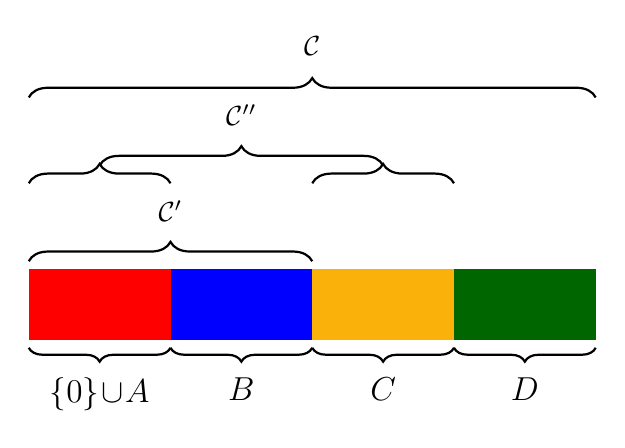
\begin{tikzpicture}[xscale=0.9,yscale=-0.9]

\fill[red] (0,0) rectangle ++(2,1);
\fill[blue] (2,0) rectangle ++(2,1);
\fill[yellow!40!orange] (4,0) rectangle ++(2,1);
\fill[green!40!black] (6,0) rectangle ++(2,1);

\draw [
    thick,
    decoration={
        brace,
		%mirror,
		amplitude=7pt,
        raise=0.1cm
    },
    decorate
] (0,0) -- (4,0)
node  [pos=0.5,anchor=north,yshift=1cm] {$\cC'$}; 

\draw [
    thick,
    decoration={
        brace,
		%mirror,
		amplitude=7pt,
        raise=0.1cm
    },
    decorate
] (1,-1.35) -- (5,-1.35)
node  [pos=0.5,anchor=north,yshift=1cm] {$\cC''$}; 
\draw [
    thick,
    decoration={
        brace,
		%mirror,
		amplitude=7pt,
        raise=0.1cm
    },
    decorate
] (0,-1.1) -- (2,-1.1);
\draw [
    thick,
    decoration={
        brace,
		%mirror,
		amplitude=7pt,
        raise=0.1cm
    },
    decorate
] (4,-1.1) -- (6,-1.1);

\draw [
    thick,
    decoration={
        brace,
		%mirror,
		amplitude=7pt,
        raise=1.1cm
    },
    decorate
] (0,-1.2) -- (8,-1.2)
node  [pos=0.5,anchor=north,yshift=2cm] {$\cC$};


\draw [
    thick,
    decoration={
        brace,
        mirror,
		amplitude=5pt,
        raise=1cm
    },
    decorate
] (4,0) -- (6,0)
node [pos=0.5,anchor=north,yshift=-1.25cm] {\large $C$}; 

\draw [
    thick,
    decoration={
        brace,
        mirror,
		amplitude=5pt,
        raise=1cm
    },
    decorate
] (6,0) -- (8,0)
node [pos=0.5,anchor=north,yshift=-1.25cm] {\large $D$}; 

\draw [
    thick,
    decoration={
        brace,
        mirror,
		amplitude=5pt,
        raise=1cm
    },
    decorate
] (2,0) -- (4,0)
node [pos=0.5,anchor=north,yshift=-1.25cm] {\large $B$}; 

\draw [
    thick,
    decoration={
        brace,
		mirror,
		amplitude=5pt,
        raise=1cm
    },
    decorate
] (0,0) -- (2,0)
node [pos=0.5,anchor=north,yshift=-1.25cm] {\large $\{0\} \!\cup\! A$}; 
\end{tikzpicture}}
\end{center}
\vspace{-2mm}
    \caption{Diagram showing the nesting structure of $\cC$, $\cC'$, and $\cC''$ with relative sizes shown for the $\RM$ code sequence.}
   \label{rm-nesting}
\end{figure}

\iffalse

\HP{Then, I would maybe cite away all definitions for $\RM$ codes and just list the properties we need with citations to where they are proved. \\
We will use the following well-known properties of $\RM$ codes:
\begin{enumerate}
\item the permutation automorphism group of any $\RM$ code is doubly transitive,
\item if $\cC = \RM (r,m+1)$, then we can choose $A = [2^m]$ and $B=[2^{m-1}]\cup\{2^{m},\ldots,2^{m}+2^{m-1}-1\}$ so that $|A|=|B|=2^m$, $\cC|_A = \cC|_B = \RM(r,m)$ and $A\cap B = [2^{m-1}]$,
\item add any necessary rate conditions
\end{enumerate}}

\AM{we also have to use $A,B,C,D$ it seems}.

The Reed--Muller code $\RM$ ( r,m)$ is a length-$N=2^{m}$ binary linear code with rate 
\begin{align*}
    R(r,m)=\frac{1}{2^m}\sum_{i=0}^{r}{m\choose i}.
\end{align*}
The generator matrices $G_{r,m}$ for $\RM$ ( r,m)$ codes satisfy the recursion \vspace{-1.5mm}
\[
G_{r,m+1}=\begin{bmatrix} G_{r,m} & G_{r,m} \\ 0 & G_{r-1,m} \end{bmatrix}  %\quad \text{from } G_{-1,m} = \text{empty}, \;  G_{r,0} = [1] \text{ for } r\geq0
\vspace*{-1mm}\]
Let the set of $m$-variate polynomials with coefficients in $\mathbb{F}_{2}$ and degree at most $r$ be $\cF (r,m)$.
 $\RM(r,m)$ is constructed by evaluating each polynomial in $\cF(r,m)$ at all points $\bx \in \mathbb{F}_2^m$ to get
\[ \RM(r,m) \coloneqq \left\{ \bc\in\mathbb{F}_{2}^{n}\,\middle|\,f\in\mathcal{F}(r,m),\,c_{\ell}=f\big(\theta_{m}(\ell)\big),\ell\in[n]\right\}, \]
where we define $\theta_{m}\colon[n]\to\mathbb{F}_{2}^{m}$ to be the bijective function that maps the integer $\ell\in[n]$ to its binary expansion $ \bb\in\mathbb{F}_{2}^{m}$.
We assume that $b_{0}$ is the LSB and $b_{m-1}$ is the MSB and, for example, this implies that $\theta_{5}(20)=(1,1,0,0,1)$. 
RM codes have rich symmetry properties. For our proofs, we will heavily use their transitive, doubly transitive symmetry and nesting properties \cite{Reeves-it23}.

% Let $S_n$ be the set of permutations (i.e, bijective functions) mapping
% $[n]$ to itself. The symmetry group of a random vector $X = (X_0, . . . , X_{n-1})$ is defined to be
% \begin{align*}
%     \mathcal{G} := \{\pi \in S_n : (X_{\pi(0)}, . . . , X_{\pi(n-1)})
% \stackrel{d}{=} X\}
% \end{align*}
% where $\stackrel{d}{=}$ refers to  equality in distribution. The symmetry group $\mathcal{G}$ is transitive if $\forall i,j\in [n],$ there is a $\pi \in \mathcal{G}$ such that $\pi(i)=j$. The symmetry group $\mathcal{G}$ is doubly-transitive if for distinct $i,j,k\in [n]$, there is a $\pi \in \mathcal{G}$ such that $\pi(i)=i$ and $\pi(j)=k$.


The nesting property of $\RM$ codes  says that longer
RM codes can be punctured down to shorter $\RM$ codes of
the same order. For a code $\cC \subseteq \cX^n$, we define its projection onto a subset $A \subseteq [n]$ of its coordinates by \vspace{-1.5mm}
\[ \cC |_A \coloneqq \{ \bc_A \in \cX^{|A|} \, | \, \bc \in \cC \}. \]
A code $\cC' \subseteq \cX^{|A|}$ is said to be nested inside $\cC$ at $A$ if $\cC|_A = \cC'$. There are nested copies of $\RM$ ( r,m-k)$ inside $\RM$ ( r,m)$ for $k\leq m-r$. The above figure shows $\RM$ ( r,m)$ which is supported  indices $I_{\cC}=\{0\} \cup A\cup B \cup C\cup D$, while two $\RM$ ( r,m-1)$ are supported on the indices $I_{\cC'}=\{0\} \cup A\cup B$ and $I_{\cC''}=\{0\} \cup A\cup C$ respectively.
% \AM{added details on nesting from jtg}
\fi


\subsection{Symmetric Binary-Input Classical-Quantum Channels}

A classical-quantum (CQ) channel $W \colon \cX \to \cD$ defined by $x \mapsto \rho^x$ takes a classical binary input $x\in \mathcal{X}$ and produces a quantum state represented by the density matrix $\rho^x$. For the classical input distribution $P_{X}(x)$, the associated classical quantum $\rho_{XY}$ is denoted by 
\begin{align*}
    \rho_{XY}=\sum_{x} P_{X}(x) \big(\ketbra{x}{x}_{X}\otimes \rho^{x}_{Y} \big).
\end{align*}
The Holevo information is the maximum amount of information that can be obtained about $X$ from $Y$ and is given by \vspace*{-2mm}
\begin{align*}
    I(X;Y)_{\rho_{XY}} = S\left(\sum_{x\in \cX}p_{\mathcal{X}}(x)\rho^{x}\right)-\sum_{x\in \cX}p_{\mathcal{X}}(x)S(\rho^x),
\end{align*}
where $S(\rho)=-\Tr(\rho\log \rho)$ is the von-Neumann entropy.
\begin{defn}
A binary-input CQ channel $W\colon\{0,1\}\rightarrow \mathcal{D}$ is defined by $x \mapsto \rho^x$.
%which maps the binary classical input $x\in\{0,1\}$ to the density matrix $W(x)\in\mathcal{D}^n$ of the quantum output.
If there is a unitary $U$ satisfying $U^{2}=\mathbb{I}$ such that $\rho^1=U\rho^0U^\dagger$, then we call this a binary-input symmetric CQ (BSCQ) channel. 
\end{defn}
For the BSCQ channel $W$ with quantum output states $\rho^0$ and $\rho^1$ and input distribution $(1-p,p)$, we will use the following quantities for our analysis: the Holevo information $I(W) \coloneqq I(X;Y)_{\rho_{XY}}$, the channel entropy $H(W) \coloneqq H(X|Y)_{\rho_{XY}}$, the conditional min-entropy $H_{\min}(W)$ and the Helstrom error probability $P_{e}(\rho^0,\rho^1,p)$. \ifisit
A detailed description of these quantities and their relations can be found in the extended version~\cite[Section~\ref{BSCQ measures}]{Mandal-arxiv25}.  \fi
\ifarxiv
A detailed description of these quantities and their relations can be found in Appendix~\ref{BSCQ measures}.
\fi
% For the BSCQ channel $W$ with quantum output states $\rho^0$ and $\rho^1$ and input distribution $(1-p,p)$, the Holevo information $I(W)$, is \vspace*{-1mm}
% denoted by %(or the mutual information $I(X;Y)_{\rho_{XY}}$) can be derived as 
% \begin{align*}
%     I(W) \coloneqq I(X;Y)_{\rho_{XY}}=S((1-p)\rho^0+p\rho^1)-S(\rho^0)
% \end{align*}
% where we used the fact that the von-Neumann entropy is unitarily invariant i.e. $S(\rho^1)=S(\rho^0)$.
% Likewise, the channel entropy $H(W)$ is denoted by
% \begin{align*}
%     H(W) &\ \coloneqq  H(X|Y)_{\rho_{XY}}\\
%     &\ =H(X)_{\rho_{XY}}+H(Y|X)_{\rho_{XY}}-H(Y)_{\rho_{XY}}\\
%     &\ =h_{2}(p)-I(W),
% \end{align*}
% where $h_{2}(p)=-p\log_2 p-(1-p)\log_2(1-p)$ is the binary entropy function.
% Similarly, the conditional min-entropy is denoted by \vspace*{-2mm}
% \begin{align*}
%     H_{\min}(W) &\ = H_{\min}(X|Y)_{\rho_{XY}}\\
%    &\ =-\log_2\left(\frac{1}{2}+\frac{1}{2} \left\| (1-p)\rho^{0}-p\rho^{1} \right\|\right)
% \end{align*}

% % \AM{To Do: discuss min entropy}

% % \HP{Only if you you will use it.}

% % \HP{Usually $p$ is the probability of 1.}
% %\AM{Yeah, that works as well}
% \ifarxiv
% \begin{defn}
% An $m$-outcome \emph{projective measurement} of a quantum system in $\mathcal{H}_n$ is defined by a set of $m$ orthogonal projection matrices $\Pi_{j} \in \mathbb{C}^{n\times n}$ satisfying $\Pi_{i}\Pi_{j}=\delta_{i,j}\Pi_{i}$ and $\sum_{j}\Pi_{j}=\mathbb{I}_{n}$, where $\mathbb{I}_n$ is the $n\times n$ identity matrix.
% We denote such a measurement by $\hat{\Pi}=\{\Pi_{j}\}|_{j=1}^{m}$.
% \end{defn}

% Applying the measurement $\hat{\Pi}$ to the quantum state $\rho$ results in a random outcome $J$ and the probability of the event $J=j$ is given by $\text{Tr}(\Pi_{j}\rho)$.
% The post-measurement state, conditioned on the event $J=j$, is given by $\Pi_{j}\rho\Pi_{j}/ \text{Tr}(\Pi_{j}\rho)$.

% Consider a hypothesis test to distinguish between $m$ possible quantum states defined by $ \Phi = \{p_j,\rho_{j}\} |_{j=1}^{m}$, where the $j$-th hypothesis has prior probability $p_j$ and density matrix $\rho_j$.
% For a projective measurement $\hat{\Pi}$, where $\Pi_j$ is associated with hypothesis $\rho_j$, the probability of choosing correctly is \vspace{-1mm}
% \begin{align*}
%     P(\Phi,\hat{\Pi}) =\sum_{j=1}^m p_{j}\text{Tr}(\Pi_{j}\rho_{j}). \vspace*{-1mm}
% \end{align*}
% \fi
% \begin{defn} [Helstrom measurement]
% Consider the measurement that distinguishes between two quantum states $\rho^{0},\rho^{1}\in\dop^d$ when $\rho^0$ has prior  probability $1-p$.
% This measurement minimizes the error probability~\cite{helstrom1969quantum} by using projection operators onto the positive and negative eigenspaces of \[D=(1-p)\rho^{0}-p\rho^{1}.\]
% Formally, it is defined by $\hat{\Pi}_{H}=\{\Pi_{+},\mathbb{I}-\Pi_{+}\}$, where \vspace*{-1mm}
% \begin{align*}
%     \Pi_{+}=\sum_{\ket{v}\in \mathcal{V}_{+}}\ketbra{v}{v} \vspace*{-1mm}
% \end{align*}
% where, $\mathcal{V}_{+}=\{\ket{v} \in \hn \,|\, \braket{v}{v}=1,\exists \lambda\geq 0, D\ket{v}=\lambda \ket{v}\}$.
% The resulting ``Helstrom error probability'' is denoted by
% \begin{align*}
%     P_{e}(\rho^0,\rho^1,p) \coloneqq \frac{1}{2}-\frac{1}{2}\left\|(1-p)\rho^0-p\rho^1 \right\|_{1}.
% \end{align*}
% \end{defn}
% %The error probability for distinguishing BSCQ outputs $\rho^0,\rho^1$ with input distribution $(1-p,p)$
% %\HP{Why not $(1-p,p)$?  These number are implicitly ordered.} can be derived as 
% %\HP{I switched to only define the error probability since $P_e = 1 - P_{succ}$.}\AM{sounds good}
%  %We denote $P_{e}(\rho^0,\rho^1,p)=1-P_{succ}(\rho^0,\rho^1,p)$ as the error probability of the measurement.
%  From \cite{tomamichel2015quantum}, we know that the Helstrom error probability is also related to the min-entropy via
%  \begin{align*}
%      P_{e}(\rho^0,\rho^1,p)=1-2^{-H_{\min}(W)}.
%  \end{align*}
%  %\HP{Add citation for this.}\AM{added}
%  This relation will be useful later to bound the uniform case
% \begin{align*}
%     P_{e} \left(\rho^0,\rho^1,\frac{1}{2} \right)=\frac{1}{2}-\frac{1}{2}T(\rho^{0},\rho^{1}),
% \end{align*}
% where $T(\rho^0,\rho^1) \coloneqq \frac{1}{2} \left\|\rho^0-\rho^1 \right\|_1$ is the trace distance.

%\HP{Let's use $T$ for trace distance.}

%\HP{At some point, we should switch parentheses to \[\left(\frac{1}{2} \right)\] for all tall display expressions.}

\section{Extrinsic Information Transfer Functions}

% \HP{Move background and statements for EXIT results here and move their proofs to the appendix}\AM{added some description, should we discuss more?}

% \HP{This is good}

For the BSCQ channel $W$,
let $W_t$ denote the BSCQ channel but where the quantum output of $W$ is erased with probability $t$.
For the channel input vector $\bx = (x_0,\ldots,x_{n-1})$, the corresponding quantum output on quantum systems $\bY = (Y_0,Y_1,\ldots,Y_{n-1})$ is defined by the density matrix
\[ W_t (\bx) = W_t (x_0) \otimes W_t (x_1) \otimes \cdots \otimes W_t (x_{n-1}). \]
We will sometimes drop the $t$ subscript when $t=0$ or alternatively write $\bY (t)$ to emphasize the dependence on $t$.

Let $\cC \subseteq \cX^n$ be a length-$n$ code for this CQ channel.
For a random codeword $\bX \in \cC$, drawn according to $P_{\bX} (\bx)$, the resulting density matrix is
\[ \rho_{\bX\!\bY (t)} = \sum_{\bx \in \cC} P_{\bX} (\bx) \left( \ket{\bx}\bra{\bx} \otimes W_t (\bx) \right). \]
We follow the convention of~\cite{Wilde-2013} and denote the mutual information by
\[ I\big(\bX;\bY(t) \big)_{\rho_{\bX\!\bY (t)}} .\]


\begin{lem}\label{exit-cq}
If the automorphism group of $\cC$ is a transitive permutation group (i.e., $\cC$ has transitive symmetry), then \vspace{-1.5mm}
\begin{align*}
\frac{1}{n} I(\bX ; \bY)_{\rho_{\bX\!\bY}}
&= \int_0^1 I\big (X_0; Y_0 \mid Y_{\sim 0}(t) \big)_{\rho^0_{\bX\!\bY (t)}} \, dt, 
\end{align*}
where $\rho^{i}_{\bX\!\bY (t)}$ is density matrix for the system where $A_i$ does not experience erasures.
\end{lem}
\ifisit
    The proof of Lemma~\ref{exit-cq} can be found in the extended version~\cite[Appendix~\ref{proof-exit-cq}]{Mandal-arxiv25}.
    \fi
    \ifarxiv
     The proof of Lemma~\ref{exit-cq} can be found in Appendix~\ref{proof-exit-cq}.
    \fi
\begin{lem}\label{rate-relation-cq}
In this setting, we have
\[ H(X_0 | Y_{\sim 0} )_{\rho_{\bX\!\bY}} \leq 1 - (C-R). \]
\end{lem}
\ifisit
    The proof of Lemma~\ref{rate-relation-cq} can be found in the extended version~\cite[Section~\ref{proof-rate-relation-cq}]{Mandal-arxiv25}.\vspace*{-2mm}
    \fi
\ifarxiv
The proof of Lemma~\ref{rate-relation-cq} can be found in Appendix~\ref{proof-rate-relation-cq}.\vspace*{-2mm}
\fi
\subsection{Orthogonal Decomposition of Observables}
% \AM{Copying the stuff from 12th August version of quantum-boolean for GNS ip.}
To show a vanishing bit-error rate for $\RM$ codes on BSCQ channels we rely on a suitable choice of inner product to decompose quantum observables. For our analysis, we adopt the inner product established from  Gelfand–Naimark–Segal (GNS) construction~\cite{arveson2012invitation}. 
For $\rho \in \dop^d$ and $\obsf,\obsg \in \mathbb{C}^{d\times d}$, consider the GNS inner product on $\mathbb{C}^{d\times d}$ defined by
\[ \inner{\obsf}{\obsg}_\rho \triangleq \Tr(\obsg^{\dagger} \rho \obsf). \] 
\ifisit
More descriptions and notations about the GNS inner product can be found in the extended version~\cite[Section~\ref{GNS appendix}]{Mandal-arxiv25}.
\fi
\ifarxiv
More descriptions and notations about the GNS inner product can be found in Appendix~\ref{GNS appendix}.
\fi
% Using this inner product, one can find an orthonormal basis $\cB = \{ \basis{0}, \basis{1}, \ldots, \basis{d^2 -1} \}$ for the vector space $\hop$ over $\mathbb{R}$, where $\basis{i} \in \hop^d$ for $i \in [d^2]$ and $\basis{0} = \mI$.
% For example, one can apply Gram-Schmidt to a standard Pauli basis whose first element is $\mI$.
% Choosing $\basis{0}=\mI$ guarantees that $\inner{ \obsf }{ \basis{0} }_\rho = \inner{\obsf}{\mI}_\rho = \Tr(\rho \obsf)$. 

% % \HP{Move the closed-form orthogonal bases to appendix.  Keep the tensor extension here.}
% % Another intriguing basis, which unfortunately does not have $I$ as an element, is defined as follows.
% % \HP{Need to adjust this to use Hermitian basis elements and also correct eigenvalue normalization. For Hermitian, we can just use $\basis{ij}+\basis{ji}$ and $\iota (\basis{ij}-\basis{ji})$.}

% % \HP{Keep tex after this}
% For $n$ qudits, this construction naturally extends to $(\hn)^{\otimes n}$ via tensor products.
% First, for $\obsf,\obsg \in \hop^{d^n}$ satisfying $\obsf=\otimes_{i=0}^{n-1} \obsf_i$ and $\obsg=\otimes_{i=0}^{n-1} \obsg_i$, one can define
% \[ \inner{\obsf}{\obsg}_{\rho,n} \triangleq  \prod_{i=0}^{n-1} \inner{\obsf_i}{\obsg_i}_{\measgn} = \prod_{i=0}^{n-1} \Tr( \obsg_i^{\dagger} \measgn \obsf_i). \]
% But, this inner product defined for tensor products has a unique extension to the full space $\hop^{d^n}$ via linearity.
% In the full space, for $\obsf,\obsg \in \hop^{d^n}$, the extension satisfies
% \[ \innerwgn{\obsf}{\obsg} = \Tr(\obsg^{\dagger} \measgn \obsf). \]
% Likewise, the single-system orthonormal basis $\cB$ naturally extends to an orthonormal basis for $\hop^{d^n}$ using the inner product on the full space.
% Specifically, for $\bs \in [d^2]^n$, we define
% \[ \basis{\bs} \triangleq \basis{s_0} \otimes \cdots \otimes \basis{s_{n-1}} \]
% and observe that
% \[ \innerwgn{\basis{\bs}}{\basis{\bt}} = \prod_{i=0}^{n-1} \Tr( \basis{t_i}^{\dagger} \measgn \basis{s_i} ) = \prod_{i=0}^{n-1} \delta_{s_i,t_i} = \delta_{\bs,\bt} . \]
% The study of quantum boolean functions is closely related to the orthogonal decomposition of observables.
% Until now, most work in this area is restricted to the uniform background measure where $\rho=\mI$ \cite{montanaro2008quantum}.
% For classical boolean functions, there is a well-developed theory beyond this (e.g., $p$-biased measures). For an observable $\obsf\in \hop^{d^n}$, let $\F{\obsf}_{\bs} = \innerwgn{\obsf}{\basis{\bs}}$ so that
% \[ \obsf = \sum_{\bs \in [d^2]^n} \F{F}_{\bs} \basis{\bs}. \]
% In this context, Parseval's theorem implies that
% \[ \normwgn{\obsf}^2 = \Tr(\obsf^{\dagger} \rho^{\otimes n} F) = \sum_{\bs \in [d^2]^n} |\F{\obsf}_{\bs}|^2 . \]
% Thus, we find that
% \[ \text{Var}(\obsf)_{\measgn} = \normwgn{\obsf}^2 - \innerwgn{\obsf}{1}^2 = \sum_{\bs \in [d^2]^n : \bs \neq \bm{0}} |\F{\obsf}_{\bs}|^2 . \]

When we extend $\cB$ to an orthonormal basis for $\mathbb{C}^{d^n\times d^n}$ using the inner product on the full space, we identify each basis element $\basis{\bs}$ only using the $n$-dimensional $d^2$-ary vector $\bs$.
We say that an observable $F$ is \emph{supported} on $A \subseteq [n]$ if we can write $\obsf = \obsf_A \otimes \, \mI_{\sim A}$ where $\obsf_A \in \hop^{d^{|A|}}$ and the tensor product preserves the original order of the quantum systems.
For an arbitrary subset $A\subseteq [n]$, we define $\cS_{A}$ to be the collection of all the strings $\bs$ such that  \[\cS_{A}\triangleq \{\bs \in [d^2]^n \,|\, s_i=0, \forall i\notin A\}-\{\mathbf{0}\}. \] 
We also note that $\basis{\bs} = \basis{\bs_A} \otimes \, \basis{\bs_{\sim A}}$, where the tensor product preserves the original order of the quantum systems.

Now, we will see the benefit of choosing our single-system basis with $\Omega_{0} = \mI$.
Based on this choice, if $\obsf$ is supported on $A$, then it follows that
\begin{align*}
\F{\obsf}_{\bs}
&= \Tr\left((\obsf_A \otimes \mI_{\sim A})^{\dagger} \rho^{\otimes n} (\basis{\bs_A} \otimes \basis{\bs_{\sim A}}) \right) \\
&= \Tr\left(\obsf_A^{\dagger} \, \rho^{\otimes |A|} \, \basis{\bs_A}  \right)
\Tr\left(\mI_{\sim A}^{\dagger} \, \rho^{\otimes |\sim A|} \, \basis{\bs_{\sim A}} \right) \\
&= \begin{cases} \Tr\left(\obsf_A^{\dagger} \, \rho^{\otimes |A|} \, \basis{\bs_A}  \right) & \text{if $\bs \in \cS_A$} \\ 0 & \text{otherwise} \end{cases}
\end{align*}
because $\Tr \big(\mI_{\sim A}^{\dagger} \, \rho^{\otimes |\sim A|} \, \basis{\bs_{\sim A}} \big) = 0$ if $\bs \notin \cS_A$.

%\HP{Does $A\cup B$ mean $A\cup B$? I would prefer the standard notation.} \AM{sounds good, will update that}
 % \AM{We can move the part describing $\cS_{A}$ and $\cS_{AB}$ to section $V$ so that we can use $n$ instead of $N$.}
 % \HP{I'm ok either way but I like the idea of using $n$ for generic statements that work without the code definition. Later, we can use $N$ for code specific statements.  Thus, another approach is to make Lemma 9 more generic and move here.}
 % \AM{yeah, I think it is better to move lemma 9 here and use n for this section}
 % \AM{I think we define $\cS_{A}$ and $\cS_{AB}$ over the extrinsic space, so was suggesting of using $n=N-1$ to define them}

For a permutation $\pi\in \symn $, let $\swap_{\pi}$ be the unitary swap operator that satisfies $\swap_{\pi} \basis{\bs} \swap_{\pi}^\dagger = \basis{\pi \bs}$.
%rearranges the quantum states according to the permutation $\pi$.
Then, we define the symmetry group of a matrix $\obsf \in \mathbb{C}^{d^n\times d^n}$ to be
\begin{align*}
    \mathrm{Sym}(\obsf)\coloneqq \{\pi\in \symn \,|\,\swap_{\pi}\,\obsf\, \swap_{\pi}^{\dagger}=\obsf\}.
\end{align*}
\begin{lem}\label{observable-symmetry}
    For $\pi\in \mathrm{Sym}(\obsf)$ % where $\mathrm{Sym}(\obsf)$ is the symmetry group for observable $\obsf$
    and $\bm{s}\in [d^{2}]^n$, we have 
    \begin{align*}
        \F{\obsf}_{\pi \bm{s}}=\F{\obsf}_{\bm{s}} 
    \end{align*}
\end{lem}
\ifisit
The proof of Lemma~\ref{observable-symmetry} can be found in the extended version~\cite[Appendix~\ref{proof-observable-symmetry}]{Mandal-arxiv25}.
\fi
\ifarxiv
The proof of Lemma~\ref{observable-symmetry} can be found in Appendix~\ref{proof-observable-symmetry}
\fi
% \begin{proof}
%     Notice that $\swap_{\pi}\measgn \swap_{\pi}^{\dagger}=\measgn$ $\forall \pi \in \symn$.
% Then expanding $\F{\obsf}_{\pi\bm{s}}$ using GNS decomposition for basis element $\Omega_{\pi \bm{s} }$, observable $\obsf$ and measure $\measgn$ we have
% \begin{align*}
%     \F{\obsf}_{\pi\bm{s}} &\ =\Tr(\obsf^{\dagger}\measgn \Omega_{\pi \bm{s}})\\
%     &\ =\Tr(\swap_{\pi}\obsf^{\dagger}\swap_{\pi}^{\dagger}\measgn \swap_{\pi}\Omega_{\bm{s}}\swap_{\pi}^{\dagger})\\
%     &\ = \Tr(\obsf^{\dagger}\measgn\Omega_{\bm{s}})\\
%     &\ =\F{\obsf}_{\bm{s}} . \qedhere
% \end{align*}
% \end{proof}

%\HP{Here is prototype of how we could state the transitive lemma before introducing RM.  One benefit is that this lemma by itself may be useful to others. }
%\AM{yeah , that makes sense}
\begin{lem}\label{cq-transitiveQ}
    For disjoint sets $A,B,C\subseteq[n]$ with $|B|=|C|$ and $\kappa=|A|/(|A|+|B|)$, let $\obsf$ and $\obsg$ be observables supported $A\cup B$ and $A \cup C$, respectively.
    Suppose there is a permutation $\pi \in S_n$ such that $\pi(i) = i$ for $i \in A$ and $\swap_{\pi} \, F \, \swap_{\pi}^\dagger = G$.
    Then, if $\mathrm{Sym}(F_{AB})$ is transitive, we have 
    \begin{align*}
      \innerwgn{\obsf}{\obsg} & \leq \kappa\normwgn{\obsf}^{2}
         +(1-\kappa)\left\langle \obsf , \mI \right\rangle_{\rho^{\otimes n}}^{2}.
    \end{align*}
\end{lem}
\ifisit
    The proof of Lemma~\ref{cq-transitiveQ} can be found in the extended version~\cite[Appendix~\ref{proof-cq-transitiveQ}]{Mandal-arxiv25}.
    \fi
    \ifarxiv
    The proof of Lemma~\ref{cq-transitiveQ} can be found in  Appendix~\ref{proof-cq-transitiveQ}.
    \fi
%\HP{Next def would be in proof of lemma}
%Similarly, for $A, B\subset [N]$, we define $\cS_{AB}=\{\bs \in [d^2]^n \,|\, s_i=0,\forall i\notin A\cup B\}-\{\bm{0}\}$.



While our analysis is based on the GNS inner product, most of the ideas (e.g., the above lemma) extend naturally to the Kubo-Martin-Schwinger (KMS) inner product \cite{olkiewicz1999hypercontractivity}. This is discussed in
\ifarxiv Appendix~\ref{kms}\fi
\ifisit \cite[Appendix~\ref{kms}]{Mandal-arxiv25} \fi.\\

% \AM{not sure if it is the best citation}
% \HP{For a more complete treatment, you might try "Hypercontractivity in noncommutative lpspaces" by R Olkiewicz, B Zegarlinski.}
\vspace*{-3mm}
\section{Minimum Mean-Squared Error (MMSE) for Quantum Binary Hypothesis Testing}

%\HP{In this section, we use $V$ for a unitary and $v_i$ for its columns.  This is a local definition, so I think it's fine to use $V_{\bs}$ later for the basis.  What do you think?}
%\AM{what about $\cV_{\bs}$ for basis}
%\HP{That's a possibility but I like to keep the basic font/shape for objects of the same type.  Since we use $F,G$ for observables, I like $V_{\bs}$ for the basis.}
%\AM{that sounds good}
\iffalse
\HP{Put next section in appendix to give general MMSE def?}
\subsection{MMSE for CQ States}
For a CQ state with classical random variable $X \in \{x_0,\ldots,x_{k-1}\} \subseteq \mathbb{R}$ and a quantum system $Y$, the density matrix is given by
\[ \rho_{XY} = \sum_{i \in [k]} \pr{X=x_i} \left( \ket{i}\bra{i} \otimes \rho_{Y}^{x_i} \right), \]
where $\rho_{Y}^{x_i}$ is the density matrix of the system $Y$ given $X=x_i$.
Using this, the MMSE of $X$ given $Y$ equals
\[ \mmse(X|Y)_{\rho_{XY}} = \min_{M}  ... \]
\fi

\subsection{MMSE Achieving Observable}

For a BSCQ $W$ with input distribution $(1-p,p)$, we can combine the input and output into the binary CQ state
\begin{align*}
    \rho_{XY} = (1-p) \ket{0}\bra{0}_{ X} \otimes \rho^0_{Y} + p \ket{1}\bra{1}_{X} \rho^{1}_{Y} ,
\end{align*}
where $\rho^0,\rho^1 \in \dop^{d}$.
Let $\obs_X = (\ket{0}\bra{0}_X - \ket{1}\bra{1}_X)\otimes \mI_Y$ be the quantum observation of $X$ and $\obs_{Y} = \mI_X \otimes \measo_Y$ be any observable of the quantum systems $X$ and $Y$.
% \AM{I think $O_{X}$ and $O_{Y}$ contradict the way we defined notations before, what are the good alternatives?}
%\HP{Here, I wonder if we should use $M$ instead of $\measo$?  I know this conflicts with the MMSE in the other paper but we can just use something like $\mathrm{MMSE} (\cC_k)$ or even $\cM(\cC_k)$}
%\AM{yeah, that works better}
Define $\rho_Y = \Tr_X (\rho_{XY})=(1-p)\rho^0+p\rho^1$ and $D = (1-p) \rho^0- p \rho^1$.
Then, the mean-squared error (MSE) associated with the observable $\obs_Y$ (defined in terms of $\measo_Y$)
%for CQ state $\rho_{XY}$ as an estimator for $X$
is given by
\begin{align*}
    \mse(\rho_{XY},\measo_Y) &\ \coloneqq \Tr \big(\rho_{XY} (\obs_X - \obs_Y)^2 \big) \\
    &\ = \Tr \big(\rho_{XY} (\obs_X^2 - 2 \obs_X \obs_Y + \obs_Y^2 )\big)\\
    &\ = 1 - 2 \Tr ( D \measo_Y ) + \Tr(\rho_Y \measo_Y^2).
\end{align*}

Thus, the minimum mean-squared error (MMSE) is found by optimizing over $\measo_Y$. Let the spectral decomposition $D = V \Lambda_D V^{\dagger}$, $d_i = [\Lambda_D]_{ii}$ be $i$-th eigenvalue of $D$ and $p_i = [V^{\dagger} \rho_Y V]_{ii} = \bra{v_i} \rho_Y \ket{v_i}$ and $[\Lambda_{\measo} ]_{ii} = \frac{[V^{\dagger} D V]_{ii}}{[V^{\dagger} \rho_Y V]_{ii}} = \frac{d_i}{p_i} $.
\begin{lem}\label{mmse-observable}
     Consider a CQ state $\rho_{XY}$ with observables $\obs_X$, % = (\ket{0}\bra{0}_X - \ket{1}\bra{1}_X)\otimes \mI_Y$,
     $\obs_{Y}$ %$=\mI_{X}\otimes \measo_{Y}$,
     and $\measo_{Y}$ defined as above.
     %being any arbitrary observable in quantum system $Y$ and $\mse(\rho_{XY},\measo_Y)  = \Tr \big(\rho_{XY} (\obs_X - \obs_Y)^2 \big)$, 
     Then, the observable $\measo_{Y}^* = V \Lambda_{\measo} V^{\dagger}$ minimizes the MSE $\mse(\rho_{XY},\measo_Y)$ and is called the MMSE observable. %we call the observable $\measo_{Y}^*$ the \emph{MMSE observable} associated with the MSE to predict binary input in $X$ from the quantum observation in $Y$.
     The MSE attained by $\measo_{Y}^*$ is called \emph{MMSE} and denoted by $\mmse(X|Y)_{\rho_{XY}}$.
     Thus, we have
    \begin{align*}
    &\ \measo_Y^*  = \arg \min_{\measo_Y}\mse(\rho_{XY},\measo_{Y})\\
    &\    \mmse(X|Y)_{\rho_{XY}} =\mse(\rho_{XY},\measo_Y^{*}).
    \end{align*}
\end{lem}
\ifisit
 The proof of Lemma~\ref{mmse-observable} can be found in the extended version~\cite[Appendix~\ref{proof-mmse-observable}]{Mandal-arxiv25}.
 \fi
 \ifarxiv
 The proof of Lemma~\ref{mmse-observable} can be found in Appendix~\ref{proof-mmse-observable}
 \fi
% By treating $f$ as a mapping from the Hilbert space of observables (containing $\measo_Y$) to the real numbers, the gradient $\nabla f$ can be defined using the Hilbert-Schmidt inner product and the condition $\mse(\rho_{XY},\measo_Y+Q_Y) = \mse(\rho_{XY},\measo_Y) + \inner{Q_Y}{\nabla \mse(\rho_{XY},\measo_Y)}_{\mathrm{HS}} + o(\|Q_Y\|)$ as $\| Q_Y \| \to 0$.
% It follows that the gradient is given by the expression
% \[ (\nabla \mse) (\rho_{XY},\measo_Y) = \big( -2 D + \rho_Y \measo_Y + \measo_Y \rho_Y \big)^{\dagger}.\]

% From the spectral decomposition $D = V \Lambda_D V^{\dagger}$, we can evaluate the MSE for the choice
% $\measo_Y = V \Lambda_{\measo} V^{\dagger}$ where $\Lambda_{\measo}$ is determined later.
% It follows that
% \[ \mse(\rho_{XY},V \Lambda_{\measo} V^{\dagger}) = 1 - 2 \Tr (\Lambda_{\measo} \Lambda_D) + \Tr (V^{\dagger} \rho_Y V \Lambda_{\measo}^2 ). \]
% Let $d_i = [\Lambda_D]_{ii}$ be $i$-th eigenvalue of $D$ and $p_i = [V^{\dagger} \rho_Y V]_{ii} = \bra{v_i} \rho_Y \ket{v_i}$ be the probability that the outcome of the $\measo_Y$-observable is associated with $i$-th eigenvector of $D$.
% Minimizing the MSE over $\Lambda_P$ gives the stationary condition
% \begin{equation}  \label{eq:Mstar_spectral}[\Lambda_{\measo} ]_{ii} = \frac{[V^{\dagger} D V]_{ii}}{[V^{\dagger} \rho_Y V]_{ii}} = \frac{d_i}{p_i} .
% \end{equation}

% Now, we verify that $\measo_Y^* = V \Lambda_{\measo} V^{\dagger}$ is a stationary point by evaluating the derivative at $\measo_Y^*$ in the direction $Q_Y$.
% Since $\measo_Y^*$ must be Hermitian, the perturbation $Q_Y$ must also be Hermitian and the orthogonal decomposition $Q_Y = \sum\nolimits_{i,j} q_{ij} \ket{v_i}\bra{v_j}$ will be useful.
% Putting things together, we find that
% \begin{align*}
% &\ \inner{Q_Y}{\nabla \mse (\rho_{XY},\measo_Y^*)}_{\mathrm{HS}}\\
% &= \inner{Q_Y}{\big( -2 D + \rho_Y\measo_Y^* + \measo_Y^* \rho_Y \big)^{\dagger}}_{\mathrm{HS}} \\
% &= -2 \Tr(D Q_Y) + \Tr(\rho_Y V \Lambda_{\measo} V^H Q_Y )\\
% &\ \quad + \Tr(V \Lambda_{\measo} V^{\dagger} \rho_Y Q_Y )\\
% &= -2 \Tr(D \sum\nolimits_{i,j} q_{ij} \ket{v_i}\bra{v_j}) \\
% &\ \quad+ \Tr(\rho_Y V \Lambda_{\measo} V^{\dagger}\sum\nolimits_{i,j} q_{ij} \ket{v_i}\bra{v_j} )\\
% &\ \quad + \Tr(V \Lambda_{\measo} V^{\dagger} \rho_Y \sum\nolimits_{i,j} q_{ij} \ket{v_i}\bra{v_j} )\\
% &= \sum_{ij}  \left( -2 \delta_{i,j} q_{ij} d_i + \delta_{i,j} q_{ij} p_i \frac{d_i}{p_i} + \delta_{i,j} q_{ij} p_i \frac{d_i}{p_i} \right) \\
% &= 0.
% \end{align*}
% Thus, the observable $\measo_Y^*$ minimizes the MSE.
% \begin{defn}
%     For a CQ state $\rho_{XY}$, observables $\obs_X = (\ket{0}\bra{0}_X - \ket{1}\bra{1}_X)\otimes \mI_Y$, and $\obs_{Y}=\mI_{X}\otimes \measo_{Y}$, with $\measo_{Y}$ being any arbitrary observable in quantum system $Y$ and $\mse(\rho_{XY},\measo_Y)  = \Tr \big(\rho_{XY} (\obs_X - \obs_Y)^2 \big)$, we call the observable $\measo_{Y}^*$ the \emph{MMSE observable} associated with the MSE to predict binary input in $X$ from the quantum observation in $Y$. The MSE error attained at $\measo_{Y}^*$ is called \emph{MMSE} for the CQ state $\rho_{XY}$ which we denote as $\mmse(X|Y)_{\rho_{XY}}$ i.e.
%     \begin{align*}
%     &\ \measo_Y^*  = \arg \min_{\measo_Y}\mse(\rho_{XY},\measo_{Y})\\
%     &\    \mmse(X|Y)_{\rho_{XY}} =\mse(\rho_{XY},\measo_Y^{*}).
%     \end{align*}
% \end{defn}
%\HP{We could also use $\measo_Y^*$ here for the MMSE observable.  This might be more standard and avoid hats later. Though, while we're using $A^\dagger$ for $A^H$, many papers use $A^*$. }
%\AM{if we are going to use $\measo_Y^*$ for the MMSE observable, $A^{\dagger}$ is probably better choice for $A^H$.}
%\HP{Yes, I think we're already using $A^\dagger$ and we should keep this.}

% While Helstrom measurement to distinguish $\rho^0$ and $\rho^1$ is formed by grouping the eigenvectors associated with positive and negative eigenspaces of $D$ respectively, the MMSE observable is constructed by attaching weights $\{\frac{d_i}{p_i}\}_{i=0}^{d-1}$ to the eigenvectors $\{\ket{v_i}\}_{i=0}^{d-1}$ of $D$. Intuitively these weights introduce biases for predicting 0 or 1 for input in $X$ from quantum observation in $Y$. In Lemma~\ref{mmse-p-error}, we will establish the relationship between MMSE $\mmse(X|Y)_{\rho_{XY}}$ and Helstrom error probability $P_{e}(\rho^0,\rho^1,\frac{1}{2})$ for the uniform inputs and symmetric CQ output states $\rho^0$ and $\rho^1$.

% \AM{Should we talk about the relation between $\hat{\measo}_{Y}$ and the Helstrom measurement?}
% \HP{Yes, we should probably mention that taking the sign of $\measo_Y$ gives the Helstrom measurement.}
% \AM{To Do- Add description on MMSE, relation with Helstrom, move to appendix}
\subsection{ MMSE Relation for BSCQ Channels}
\begin{lem}\label{pm-symmetry}
    Consider a BSCQ channel with outputs $\rho^{0}$ and $\rho^{1}$, where $\rho^{1}=U\rho^{0}U$ with $U^2=\mI$, and a uniform random input $X$ (i.e. $p=1/2$).
    Then, the MMSE $\mmse(X|Y)_{\rho_{XY}}$ satisfies
    %$\mse(\rho_{XY},\measo_{Y})$ with $\measo_{Y}$ being the MSE minimizing observable on system Y satisfies
    %\HP{Should we be using $\hat\measo_Y$ or $\measo_Y^*$ here.}
    %\AM{Yes, $\measo_Y^*$ fits better, will change that, I will probably describe $\mmse(X|Y)$ in the previous section by defining $\mmse(X|Y)=\mse(\rho,\measo_Y^*)$ and use $\mmse(X|Y)$ for the rest of the section. Also for mmse which one do you prefer- $\mmse(X|Y)$ or $\mmse(\rho_{XY})$  or $\mmse(X|Y)_{\rho_{XY}}$? }
    %\HP{Great. Also, your mmse notation make sense.  I think I like the last one to match mutual information.}
    \begin{align*}
    \mmse(X|Y)_{\rho_{XY}} & =1 - 2 \Tr \left ( \left((1-p) \rho^{0} - p \rho^{1}\right) \measo_{Y} \right) \\
    &\ \quad + \Tr\left(\left((1-p) \rho^{0} + p \rho^{1} \right)\measo_{Y}^2\right)\\
    & = 1- 2 \Tr \left ( \rho^{0}  \measo_{Y} \right)+\Tr\left( \rho^{0} \measo_{Y}^2\right)\\
    & = \Tr (\rho^{0}(\mI_{Y}-\measo_{Y})^2).
\end{align*}
\end{lem}
\ifisit
The proof of Lemma~\ref{pm-symmetry} can be found in the extended version~\cite[Appendix~\ref{proof-pm-symmetry}]{Mandal-arxiv25}.
\fi
\ifarxiv
The proof of Lemma~\ref{pm-symmetry} can be found in Appendix~\ref{proof-pm-symmetry}
\fi
% \begin{proof}
    
% Expanding $D$ and $\measo_{Y}$ using the spectral decomposition from \eqref{eq:Mstar_spectral}, we get
% \begin{align*}
%      \mmse(X|Y)_{\rho_{XY}} & =1 - 2 \Tr \left ( \left((1-p) \rho^{0} - p \rho^{1}\right) \measo_{Y} \right) \\
%      &\ \quad + \Tr\left(\left((1-p) \rho^0 + p \rho^1 \right)\measo_{Y}^2\right)\\
%     & = 1-\sum_{i=0}^{d-1}\frac{d_{i}^2}{p_{i}} .
% \end{align*}
% Define $\bra{v_i}\rho^{0}\ket{v_i}=p_{i}^0$ and $\bra{v_i}\rho^{1}\ket{v_i}=p_{i}^1$. This implies $(1-p)p_{i}^0+pp_{i}^1=p_i$ and $(1-p)p_{i}^0-pp_{i}^1=d_i$. Since, $\rho^1=U\rho^0U$ with $U^2=I$ and $p=1/2$, then $U\ket{v_i}$ is also an eigenvector of $D$ \cite{brandsen2022belief}. Let $\cR$ be the set such that 
% \begin{align*}
%     \cR\coloneqq\{(i,i')\in [d]\times [d]\,|\,\ket{v_{i'}}=U\ket{v_{i}}\}.
% \end{align*} 
% Thus we have $|\cR|=\frac{d}{2}$.
% Let $\ket{v_{i'}}=U\ket{v_i}$, then 
% \begin{align*}
% p_{i'}^0 &=\bra{v_{i'}}\rho^0\ket{v_{i'}}=\bra{v_i}U\rho^0U\ket{v_i}=p_{i}^1, \\
%  p_{i'}^1 &= \bra{v_{i'}}\rho^1\ket{v_{i'}}=\bra{v_i}U^2\rho^0U^2\ket{v_i}=p_{i}^0 , \\
%  d_{i'} &= \frac{1}{2}p_{i'}^0-\frac{1}{2}p_{i'}^{1}=-d_i .
% \end{align*}
% Then, using the above equalities we get
% \begin{align*}
%    1 - & 2 \Tr \left ( \rho^0  \measo_{Y} \right)+\Tr\left( \rho^0 \measo_{Y}^2\right)\\
%    & = 1-2\sum_{i=0}^{d-1}p_{i}^0\frac{d_i}{p_i}+\sum_{i=0}^{d-1}p_{i}^0 \left(\frac{d_{i}}{p_{i}}\right)^{2}\\
%     & = 1- \!\!\! \sum_{(i,i')\in \cR} \! \left(2p_{i}^0\frac{d_i}{p_i}+2p_{i'}^0\frac{d_i'}{p_i'}-p_{i}^0\left(\frac{d_{i}}{p_{i}}\right)^{2} \!\!\! -p_{i'}^0\left(\frac{d_{i'}}{p_{i'}}\right)^{2}\right)\\
%     & = 1- \!\!\!\sum_{(i,i')\in \cR} \! \left(2p_{i}^0\frac{d_i}{p_i}-2p_{i}^1\frac{d_i}{p_i}-p_{i}^0\left(\frac{d_{i}}{p_{i}}\right)^{2} \!\!\! -p_{i}^1\left(\frac{d_{i}}{p_{i}}\right)^{2}\right)\\
%     & \stackrel{(a)}{=} 1- \!\! \sum_{(i,i')\in \cR}\left(4\frac{d_i^{2}}{p_i}-2\frac{d_{i}^{2}}{p_{i}}\right)\\
%     & \stackrel{(b)}{=} 1- \!\! \sum_{(i,i')\in \cR}\left(\frac{d_{i}^{2}}{p_{i}}+\frac{d_{i'}^{2}}{p_{i'}}\right)\\
%     & = \mmse(X|Y)_{\rho_{XY}},
% \end{align*}
% % \HP{I suggest giving $i,i':\ket{v_{i'}}=U\ket{v_{i}}$ a name in order to save space and clarify summation sets for $i,i'$.}
% % \AM{what about now?}
% % \HP{Great!}
% where $(a)$ follows from the fact that $\frac{p_{i}^{0}-p_{i}^{1}}{2}=d_i$, $\frac{p_{i}^{0}+p_{i}^{1}}{2}=p_i$ and $(b)$ holds because $d_{i'}=-d_{i}$ and $p_{i'}=p_i$.
% \end{proof}
% \begin{rem}
% From this, we observe that
% \begin{align*}
%     \Tr \left ( \rho^0 \measo_{Y} \right)= \Tr \left ( \rho^0  \measo_{Y}^2 \right)=\sum_{i}\frac{d_{i}^2}{p_{i}}=1-\mse(\measo_{Y}).
% \end{align*}
% \end{rem}
   

 \begin{lem}\label{mmse-p-error}
    Consider a BSCQ with outputs $\rho^{0}$ and $\rho^{1}$, where $\rho^{1}=U\rho^{0}U$ with $U^2=\mI$, and a uniform random input $X$ (i.e. $p=1/2$).
    Then, the MMSE $\mmse(X|Y)_{\rho_{XY}}$ satisfies
        % $\mse(\rho_{XY},\measo_{Y})$ with $\measo_{Y}$ being the MSE minimizing observable on system Y satisfies
    \begin{align*}
    \mmse(X|Y)_{\rho_{XY}} &\ \geq 2P_{e}\left(\rho^0,\rho^1,\frac{1}{2}\right)\\
    \mmse(X|Y)_{\rho_{XY}} &\ \leq 4P_{e}\left(\rho^0,\rho^1,\frac{1}{2}\right)\left(1-P_{e}\left(\rho^0,\rho^1,\frac{1}{2}\right)\right).
\end{align*}

\end{lem}
\ifisit
    The proof of Lemma~\ref{mmse-p-error} can be found in the extended version~\cite[Appendix~\ref{proof-mmse-p-error}]{Mandal-arxiv25}.
    \fi
    \ifarxiv
    The proof of Lemma~\ref{mmse-p-error} can be found in Appendix~\ref{proof-mmse-p-error}.
    \fi
    
% \begin{proof}
%     First, from the definition of trace norm and the fact $d_{i}=[\Lambda_D]_{ii}$ for $D=\frac{1}{2}(\rho^0-\rho^1)$, we get
% \begin{align*}
%     \frac{1}{2} \left\|\rho^{0}-\rho^{1} \right\|_{1}=\sum_{i=0}^{d-1}|d_{i}| .
% \end{align*}
% On the other hand, we have 
% \begin{align*}
%     \sum_{i=0}^{d-1}\frac{d_{i}^{2}}{p_{i}} & \geq \frac{(\sum_{i=0}^{d-1}|d_{i}|)^{2}}{\sum_{i=0}^{d-1}p_{i}} \quad (\text{using Cauchy-Schwarz})\\
%     & =\frac{1}{4} \left\|\rho^{0}-\rho^{1} \right\|_{1}^{2} \quad (\text{since $\textstyle{\sum_{i=0}^{d-1}} p_{i}=1$}) .
%     \end{align*}
% %\HP{We should clarify summation range for $i$.  Also, why $\{ \cdot \}$ instead of $( \cdot )$ for comments}
% Thus, applying this inequality to $\mmse(X|Y)_{\rho_{XY}}$, we get
% \begin{align*}
%   \mmse (X|Y&)_{\rho_{XY}} = 1-  \sum_{i=0}^{d-1}\frac{d_{i}^{2}}{p_{i}}\\
%   & \leq 1- \frac{1}{4} \left\|\rho^{0}-\rho^{1} \right\|_{1}^{2} \\
%   & = \left(1+ \frac{1}{2} \left\|\rho^{0}-\rho^{1} \right\|_{1} \right)\left(1- \frac{1}{2} \left\|\rho^{0}-\rho^{1} \right\|_{1} \right)\\
%   & = 4\left(\frac{1}{2}-\frac{1}{4} \left\|\rho^{0}-\rho^{1} \right\|_{1}\right)\left(\frac{1}{2}+\frac{1}{4} \left\|\rho^{0}-\rho^{1} \right\|_{1}\right)\\
%   & = 4P_{e}\left(\rho^{0},\rho^{1},\frac{1}{2}\right)\left(1- P_{e} \left(\rho^{0},\rho^{1},\frac{1}{2} \right) \right). \qedhere
% \end{align*}
% \end{proof}
% $tr(|\rho^{1/(2p)} F \rho^{1/(2p)} |^p),tr(|\rho^{1/(2p)} F \rho^{1/(2p)} |^p)
% tr(|\rho^{1/4} F \rho^{1/4)} |^2) = <F,F>_{KMS}^2
% tr(|F|^p \rho)$

\section{Reed-Muller Codes over BSCQ Channels}\label{rm-cq-decoding}

Since $\RM$ codes are transitive and we consider transmission over memoryless BSCQ channels, any performance metric for a single bit must take the same value for all bits.
Thus, without loss of generality, we focus on bit 0 for our analysis.
Recent analyses of $\RM$ codes over classical BMS channels are based on finding an appropriate boolean function that characterizes the decodability of a single bit from the extrinsic observation~\cite{Reeves-it23,Reeves-isit23,Abbe-focs23,Pfister-arxiv25a}.
This section will introduce the necessary concepts to set up $\RM$ code decoding for a single bit from the extrinsic observation over BSCQ channels. 


%\AM{what do you think of the notations in this section}
%\HP{For density matrices, how is $\rho_\cY$ different from $\rho_{\bY}$?  I think the latter is more natural. For example, I might use $\rho_{\bX Y_{\sim 0}}$ rather than $\rho_{\cX_{\cC}\cY_{\sim 0}}$.}

%\AM{that sounds good, let me change these, for $\cC'$ input space should be the $\bX_{\{0\}\cup A\cup B}$ then?}
%
%\HP{Yes, but that's kind of ugly.  Perhaps, we define $A_0 = A\cup\{0\}$ and write $X_{A_0 B}$. BTW, I usually define things so that we drop the bold when there is a subscript (even $X_{\sim 0}$) in order to reduce bold fatigue}

Consider the $\RM$ code $\cC = \RM (r,m)$ of length $N = 2^{m}$ and $n=N-1$.
As discussed in Proposition~\ref{prop:rm_prop}c, one can partition the $n$ non-zero indices into disjoint sets $A,B,C,D\subseteq [N]\setminus \{0\}$ such that the code projections $\cC' = \cC|_{\{0\}\cup A\cup B}$ and $\cC'' = \cC|_{\{0\} \cup A \cup C}$ both equal $\RM(r,m-1)$.

Let $\bX$ denote a uniform random codeword from $\cC$ and $\bY$ denote the $N$ quantum systems that define the output when transmitting $\bX$ through independent BSCQ channels.
We use $Y_{\sim 0}$ to denote the quantum systems used for extrinsic estimation of $X_0$.
Then, the associated CQ state is given by
\begin{align*}
    \rho_{\bX Y_{\sim 0}}=\frac{1}{|\cC|}\sum_{\bm{x}\in \cC} \ketbra{\bm{x}}{\bm{x}}_{\bX}\otimes \rho^{x_{\sim 0}}_{Y_{\sim 0}},
\end{align*}
where %for $\bm{x}=\{x_0,x_1\dots,x_{n-1}\}$,
$\rho^{x_{\sim 0}}_{Y_{\sim 0}}=\rho^{x_1}_{Y_{1}}\otimes \dots \otimes \rho^{x_{n}}_{Y_{n}}$.
For codes $\cC'$, $\cC''$ the extrinsic CQ states $\rho_{X_{0\cup A\cup B}Y_{ A\cup B}}$ and $\rho_{X_{0\cup A\cup C}Y_{ A\cup C}}$ are defined  analogously.

To obtain the error probability of decoding bit-0 of $\cC$ via extrinsic observation of quantum systems $Y_{\sim 0}$, we compute
\begin{align}
    \rho_{X_0Y_{\sim 0}} &\ = \Tr_{X_{ \sim 0}}\left( \rho_{\bX Y_{\sim 0}}\right)
     = \frac{1}{2}\sum_{z\in\{0,1\}}\ketbra{z}{z}
    _{X_{0}}\otimes \overline{\rho}^{z}_{Y_{\sim 0}},
\end{align}
where 
\vspace*{-3.5mm}
\begin{align*}
  \overline{\rho}^{z}_{Y_{\sim 0}}=\frac{2}{|\cC|}\sum_{\bm{x}\in \cC,x_0=z}\rho^{x_{\sim 0}}_{Y_{\sim 0}}.
\end{align*}
Thus, the extrinsic bit-error probability for $\cC$ is given by $ P_{b}(\cC) =P_{e}\left( \overline{\rho}^{0}_{Y_{\sim 0}},  \overline{\rho}^{1}_{Y_{\sim 0}},\frac{1}{2}\right).$
% \begin{align}
%     P_{b}(\cC)&=P_{e}\left( \overline{\rho}^{0}_{Y_{\sim 0}},  \overline{\rho}^{1}_{Y_{\sim 0}},\frac{1}{2}\right).
% \end{align}
For codes $\cC'$, $\cC''$ the extrinsic CQ states $\overline{\rho}^{x}_{Y_{ A\cup B}},\overline{\rho}^{x}_{Y_{ A\cup C}}$ and bit-error probabilities $P_{b}(\cC'),P_{b}(\cC'')$ are defined analogously.

Let $\Pi_0$ and $\mI-\Pi_0$ be the projectors associated with the Helstrom measurement to distinguish $\overline{\rho}^{0}_{Y_{\sim 0}}$ and $\overline{\rho}^{1}_{Y_{\sim 0}}$. Then $P_{b}(\cC)$ satisfies \vspace*{-2mm}
\begin{align*}
    P_{b}(\cC) &\ = \frac{1}{2}\Tr\left(\left(\mI-\Pi_0\right)\overline{\rho}^{0}_{Y_{\sim 0}}\right)+\frac{1}{2}\Tr\left(\Pi_0\overline{\rho}^{1}_{Y_{\sim 0}}\right)\\
    &\ =\Tr\left(\left(\mI-\Pi_0\right)\overline{\rho}^{0}_{Y_{\sim 0}}\right)\\
    &\ \stackrel{(a)}{=} \Tr\left(\left(\mI-\Pi_0\right)(\rho^0)^{\otimes n}\right),
\end{align*}
where $(a)$ follows from channel symmetry.
% \AM{Instead of using $H(X_0|\bY_{\sim 0})$, I am using notation $H(W_{\text{extr}}^{\cC})$ to denote channel entropy for the channel to decode $x_0$ from $\bY_{\sim 0}$, what do you think?}
This shows that one can analyze the extrinsic bit-error probability by considering only the extrinsic observation from the all-zero codeword  $(\rho^0)^{\otimes n}$.

Let $W_{\text{extr}}^{\cC} \colon \{0,1\} \to \dop$ where $ x_0 \mapsto \overline{\rho}^{x_0}_{Y_{\sim 0}}$ denote the binary CQ channel associated with CQ state $\rho_{X_0 Y_{\sim 0}}$ which is the BSCQ channel corresponding to decoding bit 0 from the extrinsic quantum $Y_{\sim 0}$ using code $\cC$. 
% Then, $I(W^{\cC}_{\text{extr}})$ and $ H(W^{\cC}_{\text{extr}})$ satisfy
% \begin{align*}
%  I(W^{\cC}_{\text{extr}}) &\ =S(\frac{\overline{\rho}^{0}_{Y_{\sim 0}}+\overline{\rho}^{1}_{Y_{\sim 0}}}{2})- S(\overline{\rho}^{0}_{Y_{\sim 0}}) \\
%  H(W^{\cC}_{\text{extr}}) &\ = 1-   I(W^{\cC}_{\text{extr}})
% \end{align*}
% \HP{This seems redundant, since we've defined $H$ and $I$ for general BSCQs.}
% \AM{yeah, i commented that out, thought might be nice to restate that, but not worth the space,}

To show vanishing bit-error rate for a sequence of $\RM$ codes, our goal is to establish two relationships: (i) between $P_{b}(\cC)$ and $ H(W^{\cC}_{\text{extr}})$, (ii) between $P_{b}(\cC)$ and $P_{b}(\cC')=P_{b}(\cC'')$.
The relationship between $P_{b}(\cC)$ and $H(W^{\cC}_{\text{extr}})$ serves to determine the code rate at which decoding starts to work.
%establishes the necessary rate relations which is an essential tool for proving vanishing bit-error rate. 
The relationship between $P_{b}(\cC)$ and $P_{b}(\cC')$, $P_{b}(\cC'')$ provides a method to relate the Helstrom error probabilities for decoding bit-0 from the extrinsic observation $Y_{\sim 0}$ for $\cC = \RM(r,m)$  with the Helstrom error probabilities for decoding bit-0 from the extrinsic observations of the smaller codes $\cC'=\cC''=\RM(r,m-1)$.
%On the other hand, the relationship between $P_{b}(\cC)$ and $H(W^{\cC}_{\text{extr}})$ establishes the necessary rate relations which is an essential tool for proving vanishing bit-error rate. 

% \HP{Yes, I think that should be reduce notation and still be easy to follow.}

% \HP{Maybe use $P_b$ instead of $P_e$ to match other paper.}

% \AM{sure}
\section{Code Symmetry and Decoder Observables}\label{transitive symm obs}


%\HP{If we use superscripts, then we can write \[ O^{AB} = \sum_{s} \hat{O}^{AB}_s \basis{\bs} \]}
%\AM{what about writing it as \[ O_{AB} = \sum_{s} \hat{O}_{AB}^s \basis{\bs} ?\]}
%\HP{I now understand why you chose $\pi$ for the coefficients in Lemma 4 :-).  Maybe, we can just state that, for notational convenience, we define $F = O_{AB}$ and $G = O_{AC}$ so that  $\F{\obsf}$ and $\hat{G}$ give the Fourier coefficients.  We don't use $F,G$ anywhere in the Lemma 4 right now because $\Omega$ is the basis.  On that note, we could denote our vector space of operators with weighted inner product by $\cV$ and then use $V_{\bs}$ to denote its orthonormal basis.}
%\AM{yeah, updated the notations using $\obs$ and $\measo$, also used $\obsf=\measo_{AB}$ and $\obsg=\measo_{AC}$ for recursive bound proof, $V_{\bs}$ for the basis sounds good, will update that }

In this section, we establish recursive relations between longer and shorter $\RM$ codes using MMSE $\mmse(\cdot)$ defined in Section~\ref{rm-cq-decoding}. Let $\measo_{\sim 0}$ be the MSE minimizing observable for the extrinsic channel $W^{\cC}_{\text{extr}}$ to distinguish $\overline{\rho}^{0}_{Y_{\sim 0}}$ and $\overline{\rho}^{1}_{Y_{\sim 0}}$. Let $\hat{\measo}_{AB}$, $\hat{\measo}_{AC}$ are the MSE minimizing observables to distinguish $\overline{\rho}^{0}_{Y_{AB}}$ and $\overline{\rho}^{1}_{Y_{AB}}$ for the extrinsic channel $W^{\cC'}_{\text{extr}}$ and $\overline{\rho}^{0}_{Y_{AC}}$ and $\overline{\rho}^{1}_{Y_{AC}}$ for the extrinsic channel $W^{\cC''}_{\text{extr}}$ respectively. Let $\measo_{AB}$ be the observable realized over full extrinsic space $Y_{\sim 0}$ from the observable $\hat{\measo}_{AB}$ i.e. $\measo_{AB}=\hat{\measo}_{AB}\otimes \mI_{Y_{CD}}$. Similarly, $\measo_{AC}$ be the observable realized in $Y_{\sim 0}$  where $\measo_{AC}=\hat{\measo}_{AC}\otimes \mI_{Y_{BD}}$.
% \begin{align*}
%  \measo_{AC}= \swap_{B,C} \left(\left(\swap_{B,C} \hat{\measo}_{AC}\swap_{B,C}^{\dagger}\right)\otimes \mI_{Y_{CD}}\right)\swap_{B,C}^{\dagger}
% \end{align*}

Using the setup in Proposition~\ref{prop:rm_prop}c, let $\pi \in S_N$ be the permutation that satisfies $\pi(i) = i$ for $i\in \{0 \} \cup A \cup D$, $\pi(i) = i+2^{m-2}$ for $i\in B$, and $\pi(i) = i - 2^{m-2}$ for $i\in C$.
This permutation has the effect of swapping the $B$ and $C$ blocks in Figure~\ref{rm-nesting}.
For the unitary swap operator defined by this permutation, we use the shorthand $\swap_{BC} \coloneqq \swap_\pi$.
It follows that $\measo_{AB}=\swap_{BC}\measo_{AC}\swap_{BC}^{\dagger}$
% \begin{align*}
% \measo_{AB}=\swap_{BC}\measo_{AC}\swap_{BC}^{\dagger}
% \end{align*} 
so that $\swap_{BC}$ swaps the quantum states between the quantum systems $Y_{B}$ and $Y_{C}$ respectively.
Let $\obs_{X_0}=(\ketbra{0}{0}_{X_0}-\ketbra{1}{1}_{X_0})\otimes \mI_{Y_{\sim 0}}$ be the observable corresponding to input on $X_0$ for the extrinsic channels. Since we have defined observables $\measo_{AB},\measo_{AC}$ over the full extrinsic space  $Y_{\sim 0}$, the definition of $\obs_{X_0}$ stays the same for codes $\cC$, $\cC'$ and $\cC''$ to analyze extrinsic CQ channels. Similarly we define $\obs_{\sim 0}=\mI_{X_0}\otimes \measo_{\sim 0}$, $\obs_{AB}=\mI_{X_0}\otimes \measo_{AB}$ and $\obs_{AC}=\mI_{X_0}\otimes \measo_{AC}$. Let $\mmse(\cC)$ be the MMSE for the $\RM$ code $\cC$ corresponding to decode $X_0$ associated with extrinsic CQ channel $W^{\cC}_{\text{extr}}$. 
\ifisit
The properties of $\mmse(\cC)$, $\mmse(\cC')$ and $\mmse(\cC'')$ are discussed in the extended version~\cite[Appendix~\ref{property mmse}]{Mandal-arxiv25}.
\fi
\ifarxiv
The properties of $\mmse(\cC)$, $\mmse(\cC')$ and $\mmse(\cC'')$ are discussed in Appendix~\ref{property mmse}.
\fi
% Then $\mmse(\cC)$ satisfies
% \begin{align*}
%     \mmse(\cC) &\ = \mmse(X_0|Y_{\sim 0})_{\rho_{X_0 Y_{\sim 0}}}\\
%     % =\mse (\rho_{X_0 Y_{\sim 0}}, \measo_{\sim_0}) \\
%     &\ =\Tr\left(\rho_{X_0 Y_{\sim 0}}\left(\obs_{X_0}-\obs_{\sim 0}\right)^{2}\right)\\
%     &\ = \Tr\left(\overline{\rho}^{0}_{Y_{\sim 0}}\left(\mI_{Y_{\sim 0}}-\measo_{\sim 0}\right)^{2}\right)\\
%     &\ \stackrel{(a)}{=}\Tr\left(\meas\left(\mI_{Y_{\sim 0}}-\measo_{\sim 0}\right)^{2}\right)
% \end{align*}
% where $(a)$ follows from channel symmetry and the linearity of $\cC$.
% % \AM{do we need to prove $(a)$?}\HP{Let's ignore this detail for now and put into arXiv}.
% On the other hand $\mmse(\cC')$  satisfies 
% \begin{align*}
%     \mmse(\cC')&\ =\mmse(X_0|Y_{AB})_{\rho_{X_0Y_{AB}}}\\
%     % =\mse(\rho_{X_0 Y_{AB}},\hat{\measo}_{AB})\\
%     &\ =\Tr\left(\overline{\rho}^{0}_{Y_{AB}}\left(\mI_{AB}-\measo_{AB}\right)^{2}\right)\\
%     &\ \stackrel{(a)}{=}\Tr\left(\hat{\rho}^{0}_{Y_{AB}}\otimes \mI_{CD}\left(\mI_{Y_{\sim 0}}-\measo_{AB}\right)^{2}\right)\\
%     &\ \stackrel{(b)}{=}\Tr\left(\meas \left(\mI_{Y_{\sim 0}}-\measo_{AB}\right)^{2}\right)
% \end{align*}
% where $(a)$ is true because $\mse(\rho_{X_0 Y_{AB}},\hat{\measo}_{AB})=\mse(\rho_{X_0 Y_{AB}}\otimes \mI_{CD},\measo_{AB})$ and $(b)$ is true because $\measo_{AB}=\hat{\measo}_{AB}\otimes \mI_{CD}$.
% Similarly, $\mmse(\cC'')$ satisfies
% \begin{align*}
%   \mmse(\cC'') &\ =\mmse(X_0|Y_{AC})_{\rho_{X_0Y_{AC}}}\\
%   % =\mse(\rho_{X_0 Y_{AC}},\hat{\measo}_{AC}) \\
%   &\ =\Tr\left(\meas \left(\mI_{Y_{\sim 0}}-\measo_{AC}\right)^{2}\right).
% \end{align*}
% Since both $\cC'$ and $\cC''$ are $\RM( r,m-1)$ codes, it follows that $\mmse(\cC')=\mmse(\cC'')$.
% On the other hand from Lemma~\ref{mmse-p-error}, $\mmse(\cC)$ and $\mmse(\cC')$ satisfy 
% \begin{align*}
%     \mmse(\cC) &\ \leq 4P_b(\cC)(1-4P_b(\cC))\\
%     \mmse(\cC')&\ \leq 4P_{b}(\cC')(1-4P_b(\cC')).
% \end{align*}
Inspired by the analysis of $\RM$ codes over classical BMS channels via the two-look approach in~\cite{Pfister-arxiv25a}, we consider an extension to BSCQ channels.
In particular, we derive a recursive relationship for the extrinsic MMSE of $\RM$ codes on BSCQ channels by analyzing the observables $\measo_{AB}$, $\measo_{AC}$ and $\measo_{\sim 0}$. For this analysis the primary quantity of interest is $ \innerw{\measo_{AB}}{\measo_{AC}} $. Although the analysis of $ \innerw{\measo_{AB}}{\measo_{AC}} $ is somewhat involved, we will now show that it puts us on the right path to obtain a recursive bound for the MMSE in this setting.

Since $A,B,C\subseteq[n]$ and $|C|=|B|$, we can apply Lemma~\ref{cq-transitiveQ} to the observables $\measo_{AB}$ and $\measo_{AC}$ using the background measure $\meas$ to get \vspace*{-1.5mm}
\begin{align*}
    \innerw{\measo_{AB}}{\measo_{AC}}   &\ \leq \kappa\normw{\measo_{AB}}^{2}\\
        &\ \quad +(1-\kappa)\innerw{\measo_{AB}}{\mI}.
\end{align*}
% \begin{lem}\label{cq-transitive}
%     For $A,B,C\subseteq[n]$, $|C|=|B|$ and $\kappa=\frac{|A|}{|A|+|B|}$,
%     \begin{align*}
%       \innerw{\measo_{AB}}{\measo_{AC}}   &\ \leq \kappa\normw{\measo_{AB}}^{2}\\
%         &\ \quad +(1-\kappa)\left\langle \measo_{AB} , \mI \right\rangle_{(\rho^0)^{\otimes n}}^{2}
%     \end{align*}
%     where $\measo_{AB}$ and $\measo_{AC}$ are the observables corresponding to error events for determining  bit-$0$ of the $\RM$ code onto the quantum systems $Y_{AB}$ and $Y_{AC}$ respectively.
% \end{lem}
% \begin{proof}
% For notational convenience we denote observables $\measo_{AB}$ and $\measo_{AC}$ as $\measo_{AB}=\obsf$ and $\measo_{AC}=\obsg$. We begin with expanding $\obsf$  and $\obsg$ in $\{V_{s}\}_{s\in [d^2]^{n}}$ basis as follows
% \begin{align*}
% \obsf &\ =\F{\obsf}_{\mathbf{0}}\basis{\mathbf{0}}+\sum_{s\in \cS_{A}}\hat{\obsf}_{s}\basis{s}+\sum_{s'\in \cS_{AB}-\cS_{A} }\hat{\obsf}_{s'}\basis{s'}\\
% \obsg &\ =\hat{\obsg}_{\mathbf{0}}\basis{\mathbf{0}}+\sum_{t\in \cS_{A}}\hat{\obsg}_{t}\basis{t}+\sum_{t'\in \cS_{AC}-\cS_{A}}\hat{\obsg}_{t'}\basis{t'}
% \end{align*}
% By transitive symmetry we have, 
% \begin{align*}
% \hat{\obsf}_{\mathbf{0}}=\hat{\obsg}_{\mathbf{0}}, \quad \text{and} \quad \hat{\obsf}_{s}=\hat{\obsg}_{s},\quad \forall s\in \cS_{A}.
% \end{align*}
% Expanding$\innerw{\obsf}{\obsg}$ in $\{V_{s}\}_{s\in [d^2]^{n}}$ basis and further simplifying we get,
% \begin{align*}
%      &\ \innerw{\obsf}{\obsg} \\
%      &\ =\innerw{\sum_{s\in [n]}\hat{\obsf}_{s}\basis{s}}{\sum_{t\in [n]}\hat{\obsg}_{t}\basis{t}}\\
%      % &\=\left\langle\sum_{s\in [n]}\hat{\pi}_{s}\basis{s},\sum_{t\in [n]}\hat{\pi}'_{t}\basis{t}\right\rangle_{\rho^{\otimes n}}\\
%      &\ = 
%     \innerw{\left(\hat{\obsf}_{\mathbf{0}}\basis{\mathbf{0}}+\sum_{s\in \cS_{A}}\hat{\obsf}_{s}\basis{s}\right)}{\left(\hat{\obsg}_{\mathbf{0}}\basis{\mathbf{0}}+\sum_{t\in \cS_{A}}\hat{\obsg}_{t}\basis{t}\right)} \\
%     % &\ \left\langle\left(\hat{\pi}_{\mathbf{0}}\basis{\mathbf{0}}+\sum_{s\in S_{A}}\hat{\pi}_{s}\basis{s}\right),\left(\hat{\pi}'_{\mathbf{0}}\basis{\mathbf{0}}+\sum_{t\in S_{A}}\hat{\pi}'_{t}\basis{t}\right)\right\rangle_{\rho^{\otimes n}}\\
%     &\ \quad + \innerw{\sum_{s\in \cS_{AB}-\cS_{A}}\hat{\obsf}_{s}\basis{s}}{\sum_{t\in \cS_{AC}-\cS_{A}}\hat{\obsg}_{t}\basis{t}}\\
%      % &\  \quad  +\left\langle\sum_{s\in S_{AB}-S_{A}}\hat{\pi}_{s}\basis{s},\sum_{t\in S_{AC}-S_{A}}\hat{\pi}'_{t}\basis{t}\right\rangle_{\rho^{\otimes n}}\\
%      &\ \quad +\innerw{\left(\hat{\obsf}_{\mathbf{0}}\basis{\mathbf{0}}+\sum_{s\in \cS_{A}}\hat{\obsf}_{s}\basis{s}\right)}{\sum_{t\in \cS_{AC}-\cS_{A}}\hat{\obsg}_{t}\basis{t}}\\
%      % &\ \quad + \left\langle\left(\hat{\pi}_{\mathbf{0}}\basis{\mathbf{0}}+\sum_{s\in S_{A}}\hat{\pi}_{s}\basis{s}\right),\sum_{t\in S_{AC}-S_{A}}\hat{\pi}'_{t}\basis{t}\right\rangle_{\rho^{\otimes n}}\\
%      &\ \quad +\innerw{\sum_{s\in \cS_{AB}-\cS_{A}}\hat{\obsf}_{s}\basis{s}}{\left(\hat{\obsg}_{\mathbf{0}}\basis{\mathbf{0}}+\sum_{t\in \cS_{A}}\hat{\obsg}_{t}\basis{t}\right)}\\
%      % &\ \quad
%      %  +\left\langle\sum_{s\in S_{AB}-S_{A}}\hat{\pi}_{s}\basis{s},\left(\hat{\pi}'_{\mathbf{0}}\basis{\mathbf{0}}+\sum_{t\in S_{A}}\hat{\pi}'_{t}\basis{t}\right)\right\rangle_{\rho^{\otimes n}}\\
%      &\ = \hat{\obsf}_{\mathbf{0}}^{2} +\sum_{s\in \cS_{A}}\hat{\obsf}_{s}^{2}
% \end{align*}
% On the other hand, expanding $\normw{\obsf}^{2}$ in $\{V_{s}\}_{s\in [d^2]^{n}}$ basis we get
% \begin{align*}
%    \normw{\obsf}^{2} &\ =\hat{\obsf}_{\mathbf{0}}^{2} +\sum_{s\in \cS_{AB}}\hat{\obsf}_{s}^{2}\\
%     &\ =\hat{\obsf}_{\mathbf{0}}^{2}+\sum_{i\in A\cup B}\sum_{s \in \cS_{AB}: s_i \neq 0}\frac{\hat{\obsf}_{s}^{2}}{|s|}\\
%     &\ = \hat{\obsf}_{\mathbf{0}}^{2} + \sum_{i\in A\cup B}\eta_{i}(\obsf)
%     % &\ =\hat{\obsf}_{\mathbf{0}}^{2}+(|A|+|B|)\eta_{0}(\obsf)
% \end{align*}
% where $\eta_{i}(\obsf)=\sum_{s\in \cS_{AB}}\bm{1}_{s}(i)\frac{\hat{\obsf}_{s}^{2}}{|s|}$ and
% \begin{align*}
%     \bm{1}_{s}(i)=\begin{cases}
%         1 \quad (\text{if  $s_{i}\neq 0$})\\
%         0 \quad (\text{if $s_{i}=0$} ).
%     \end{cases}
% \end{align*}
% From the property that $\F{\obsf}_{\pi(s)}=\F{\obsf}_{s}$ $\forall \pi \in \text{Sym(F)}$ we have
% \begin{align*}
%     \eta_{\pi(i)}(\obsf) &\ =\sum_{s\in \cS_{AB}}\bm{1}_{s}(\pi(i))\frac{\hat{\obsf}_{s}^{2}}{|s|}\\
%     &\ \stackrel{(a)}{=} \sum_{s\in \cS_{AB}}\bm{1}_{\pi(s)}(\pi(i))\frac{\hat{\obsf}_{\pi(s)}^{2}}{|\pi(s)|}\\
%     &\ =\eta_{i}(\obsf).
% \end{align*}
% where $(a)$ holds from the transitive symmetry of $\RM$ codes.
% This implies that $\eta_i(\obsf)$ is independent of choice of $i$ which gives
% \begin{align*}
%     \normw{\obsf}^{2}  =\hat{\obsf}_{\mathbf{0}}^{2}+(|A|+|B|)\eta_{0}(\obsf)
% \end{align*}
% \AM{If we use $V_{s}$ for basis what notation should we use for $V_{i}(\obsf)$}\\

% \HP{Good question.  Since we only use that $V$ right here, I think we can switch to anything.  For example, we could just define a $\eta_i$ and not make this a function of $F$.}
% \AM{what about now?}\\
% % \AM{To Do:-Proof of $V_{i}(\obsf)=V_{0}(\obsf)$}
% Thus we get the following inequality
% \begin{align*}
%     \frac{|A|}{|A|+|B|}\left( \normw{\obsf}^{2}-\hat{\obsf}_{\mathbf{0}}^{2}\right) &\ = \sum_{i\in A}\eta_{0}(\obsf)\\
%     &\ \geq \sum_{i\in A}\sum_{s \in \cS_{A}: s_i \neq 0}\frac{\hat{\obsf}_{s}^{2}}{|s|}\\
%     &\ =\sum_{s\in \cS_{A}}\hat{\obsf}_{s}^{2}
% \end{align*}
% Combining the above equations we get
% \begin{align*}
%   &\ \innerw{\obsf}{\obsg} \\
%    % \left\langle O_{AB} , O_{AC} \right\rangle_{\rho^{\otimes n}} 
%    &\ \leq \hat{\obsf}_{\mathbf{0}}^{2}+ \frac{|A|}{|A|+|B|}\left( \normw{\obsf}^{2}-\hat{\obsf}_{\mathbf{0}}^{2}\right)\\
%      % &\ =\kappa \normw{O_{AB}}^{2}+(1-\kappa)\left\langle O_{AB} , I \right\rangle_{\rho^{\otimes n}}^{2}\\
%      &\ =\kappa \normw{\obsf}^{2}\\
%      &\ \qquad +(1-\kappa)\innerw{\obsf}{\mI}^{2},
% \end{align*}
% which proves the lemma.
% \end{proof}
\begin{lem} \label{recursive-cq}
For the $\RM$ code $\cC = \RM (r,m)$ and disjoint sets $A,B,C\subseteq [N]\setminus \{0\}$ such that the code projections $\cC' = \cC|_{\{0\}\cup A\cup B}$ are equal to $\RM (r,m-1)$, the MMSEs  $\mmse(\cC)$ and $\mmse(\cC')$ of the codes $\cC$ and $\cC'$ associated with decoding bit-0 from the extrinsic observations on systems $Y_{\sim 0}$ and $Y_{AB}$ satisfy \vspace*{-2.5mm}
    \begin{align*}
        \mmse(\cC)\leq \frac{1+\kappa}{2}\mmse(\cC')+\frac{1-\kappa}{2}\mmse(\cC')^{2}.
    \end{align*}
\end{lem}
\ifisit
    The proof of Lemma~\ref{recursive-cq} can be found in the extended version~\cite[Appendix~\ref{proof-recursive-cq}]{Mandal-arxiv25}.   
    \fi
    \ifarxiv
    The proof of Lemma~\ref{recursive-cq} can be found in Appendix~\ref{proof-recursive-cq}.
    \fi
% \begin{proof}
%     % Let $\tilde{\obs}_{ABC}=\mI_{X_0}\otimes \left(\frac{\measo_{AB}+\measo_{AC}}{2}\right)$. 
%     From the definition of $\mmse(\cC)$ we get 
%     \begin{align*}
%      \mmse(\cC)= &\ \mse(\rho_{X_0 Y_{\sim 0}},\measo_{\sim 0})\\
%       &\ = \Tr\left(\meas\left(\mI_{Y_{\sim 0}}-\measo_{\sim 0}\right)^{2}\right)\\
%        &\ \stackrel{(a)}{\leq} \Tr \left(\meas (\mI_{Y_{\sim 0}}-\frac{\measo_{AB}+\measo_{AC}}{2})^{2} \right)\\
%       %   & =  \Tr \left(\rho_{ABC|X=0} \left(I_{ABC}-\left(\frac{P_{AB}+P_{AC}}{2}\right)\right)^{2} \right)\\
%         &\ = \frac{1}{2}\Tr \left(\meas (\mI_{Y_{\sim 0}}-\measo_{AB})^2 \right) \\
%          &\ \quad +\frac{1}{2}\Tr \left((\mI_{Y_{\sim 0}}-\measo_{AB})\meas(\mI_{Y_{\sim 0}}-\measo_{AC}) \right)\\
%         &\ =\frac{1}{2}\mmse(\cC')+\frac{1}{2}-\frac{1}{2}\Tr\left(\meas \measo_{AB}\right)\\
%        &\ \quad -\frac{1}{2}\Tr\left(\meas \measo_{AC}\right) \\
%        &\ \quad +\frac{1}{2}\Tr\left(\measo_{AB}\meas \measo_{AC}\right)\\
%         &\ = \frac{1}{2}\mmse(\cC')+\frac{1}{2}-1+\mmse(\cC')\\
%         &\ \quad +\frac{1}{2}\Tr\left(\measo_{AB}\meas \measo_{AC}\right),
%         \end{align*}
%         where $(a)$ is true because $\measo_{\sim 0}$ is the MMSE observable.
% Applying Lemma~\ref{cq-transitiveQ}  on  $\Tr\left(\measo_{AB}\meas \measo_{AC}\right)$ we get 
% \begin{align*}
%   &\  \Tr\left(\measo_{AB}\meas \measo_{AC}\right) \\ & \leq \kappa\Tr\left(\meas \measo_{AB}^{2}\right)+(1-\kappa)\Tr\left(\meas \measo_{AB}\right)^{2}\\
%     & = \kappa \left(1-\mmse(\cC')\right)+(1-\kappa) \left(1-\mmse(\cC')\right)^{2}\\
%     & =1+(\kappa-2)\mmse(\cC')+(1-\kappa)\mmse(\cC')^{2}
% \end{align*}
% Combining the above equations we have
% \begin{align*}
%     \mmse(\cC) & = \Tr\left(\meas\left(\mI_{Y_{\sim 0}}-\measo_{\sim 0}\right)^{2}\right) \\
%     & \leq \frac{3}{2}\mmse(\cC')+\frac{\kappa-2}{2}\mmse(\cC')+\frac{1-\kappa}{2} \mmse(\cC')^{2}\\
%      & =\frac{1+\kappa}{2}\mmse(\cC')+\frac{1-\kappa}{2} \mmse(\cC')^{2}. \qedhere
% \end{align*}
% \end{proof}
% \AM{To Do:- use $\alpha$ instead of $\frac{1}{2}$}

\section{Achieving Vanishing Bit-Error Rate}
% \AM{To Do- update notations for this section}
% For $d\in \mathbb{N}$, let $[d] \triangleq \{0,1,\ldots,d-1\}$ and let $\cX = [d]$ be the input alphabet of a CQ channel $W\colon \cX \to \mathcal{D}$.

% For the BSCQ channel $W$,
% let $W_t$ denote the BSCQ channel but where the quantum output of $W$ is erased with probability $t$.
% For the channel input vector $\bx = (x_0,\ldots,x_{n-1})$, the corresponding quantum output on quantum systems $\bY = (Y_0,Y_1,\ldots,Y_{n-1})$ is defined by the density matrix
% \[ W_t (\bx) = W_t (x_0) \otimes W_t (x_1) \otimes \cdots \otimes W_t (x_{n-1}). \]
% We will sometimes drop the $t$ subscript when $t=0$ or alternatively write $\bY (t)$ to emphasize the dependence on $t$.

% Let $\cC \subseteq \cX^n$ be a length-$n$ code for this CQ channel.
% For a random codeword $\bX \in \cC$, drawn according to $P_{\bX} (\bx)$, the resulting density matrix is
% \[ \rho_{\bX\!\bY (t)} = \sum_{\bx \in \cC} P_{\bX} (\bx) \left( \ket{\bx}\bra{\bx} \otimes W_t (\bx) \right). \]
% We follow the convention of~\cite{Wilde-2013} and denote the mutual information by
% \[ I\big(\bX;\bY(t) \big)_{\rho_{\bX\!\bY (t)}} .\]


% \begin{lem}\label{exit-cq}
% If the automorphism group of $\cC$ is a transitive permutation group (i.e., $\cC$ has transitive symmetry), then \vspace{-1.5mm}
% \begin{align*}
% \frac{1}{n} I(\bX ; \bY)_{\rho_{\bX\!\bY}}
% &= \int_0^1 I\big (X_0; Y_0 \mid Y_{\sim 0}(t) \big)_{\rho^0_{\bX\!\bY (t)}} \, dt, 
% \end{align*}
% where $\rho^{i}_{\bX\!\bY (t)}$ is density matrix for the system where $A_i$ does not experience erasures.
% \end{lem}

% \begin{proof}
% First, we note that
% \begin{align*}
% I(\bX ; \bY)_{\rho_{\bX\!\bY}}
% &= H(\bX) - H(\bX | \bY)_{\rho_{\bX\!\bY}} \\
% &= H(\bX | \bY(1))_{\rho_{\bX\!\bY(1)}} - H(\bX | \bY(0))_{\rho_{\bX\!\bY(0)}} \\
% &= \int_0^1 \frac{d}{dt} H(\bX | \bY(t))_{\rho_{\bX\!\bY(t)}} \, dt. 
% \end{align*}
% Next, we assume that the erasure rate for each system is different (e.g., the erasure rate for $Y_i$ is $t_i$) and use the law of the total derivative to write
% \begin{align*}
% &\ \frac{d}{dt} H(\bX | \bY(t))_{\rho_{\bX\!\bY(\bt)}} \\
% &\ = \sum_{i=0}^{n-1} \frac{d}{dt_i} H(\bX | \bY(\bt))_{\rho_{\bX\!\bY(\bt)}} \bigg|_{t_0 = t_1 = \cdots = t_{n-1} = t},
% \end{align*}
% where $\bt = (t_0,t_1,\ldots,t_{n-1})$ is the vector of erasure rates.
% To simplify this expression, we use the chain rule of entropy and the definition of an erasure channel to write
% \begin{align*}
% &\ H(\bX | \bY(\bt))_{\rho_{\bX\!\bY(\bt)}}\\
% &\ = H(X_i | \bY(\bt))_{\rho_{\bX\!\bY(\bt)}}
% +H(X_{\sim i} | \bY(\bt),X_i)_{\rho_{\bX\!\bY(\bt)}} \\
% &\ = (1-t_i) H(X_i | Y_{\sim i} (t_{\sim i}), Y_i)_{\rho^i_{\bX\!\bY(\bt)}} \\
% &\ \quad +
% t_i H(X_i | Y_{\sim i} (t_{\sim i}))_{\rho^i_{\bX\!\bY(\bt)}} ++H(X_{\sim i} | \bY(\bt),X_i)_{\rho_{\bX\!\bY(\bt)}}
% \end{align*}
% where $\rho^{i}_{\bX\!\bY (\bt)} = \rho_{\bX\!\bY (\bt)}|_{t_i =0}$ is the density matrix of the same system except $Y_i$ does not experience erasures.
% Thus, we see that
% \begin{align*}
% &\ \frac{d}{dt_i} H(\bX | \bY(\bt))_{\rho_{\bX\!\bY(\bt)}}\\
% &= H(X_i | Y_{\sim i} (t_{\sim i}))_{\rho^i_{\bX\!\bY(\bt)}} -  H(X_i | Y_{\sim i} (t_{\sim i}), Y_i)_{\rho^i_{\bX\!\bY(\bt)}} \\
% &= I(X_i;Y_i | Y_{\sim i}(t_{\sim i}))_{\rho^i_{\bX\!\bY(\bt)}}.
% \end{align*}
% From the transitive symmetry of the code and the full permutation symmetry of the channel uses, we see that this quantity does not depend on $i$ when $t_i = t$ for all $i \in [n]$.
% By transitive symmetry, we see that this quantity does not depend on $i$ when $t_i = t$ for all $i \in [n]$.
% Thus, we observe that
% \begin{align*}
% &\ \frac{d}{dt} H(\bX | \bY(t))_{\rho_{\bX\!\bY(\bt)}}\\
% &= \sum_{i=0}^{n-1} \frac{d}{dt_i} H(\bX | \bY(\bt))_{\rho_{\bX\!\bY(\bt)}}  \bigg|_{t_0 = t_1 = \cdots = t_{n-1} = t} \\
% &= n I\big (X_0; Y_0 \mid Y_{\sim 0}(t) \big)_{\rho^i_{\bX\!\bY (t)}}.
% \end{align*}
% The proof is completed by substituting this into the integral and normalizing by $n$.
% \end{proof}

% \begin{lem}\label{rate-relation-cq}
% In this setting, we have
% \[ H(X_0 | Y_{\sim 0} )_{\rho_{\bX\!\bY}} \leq 1 - (C-R). \]
% \end{lem}



% \begin{proof}
% This follows from
% \begin{align*}
% C &= I(X_0; Y_0)_{\rho_{X_0 \! Y_0}} \\
% &= H(Y_0)_{\rho_{X_0 \! Y_0}} - H(Y_0|X_0)_{\rho_{X_0 \! Y_0}} \\
% &= H(Y_0)_{\rho^0_{\bX\!\bY(t)}} - H(Y_0|X_0,Y_{\sim 0} (t) )_{\rho^0_{\bX\!\bY (t)}} \\
% &= I(Y_0; X_0, Y_{\sim 0} (t) )_{\rho^0_{\bX\!\bY(t)}} \\
% &= I(Y_0; Y_{\sim 0}(t) )_{\rho^0_{\bX\!\bY(t)}} + I(Y_0;X_0 | Y_{\sim 0} (t))_{\rho^0_{\bX\!\bY(t)}} \\
% &\leq I(X_0; Y_{\sim 0} (t) )_{\rho^0_{\bX\!\bY(t)}} + I(Y_0;X_0 | Y_{\sim 0}(t) )_{\rho^0_{\bX\!\bY(t)}} \\
% &\leq I(X_0; Y_{\sim 0} )_{\rho_{\bX\!\bY}} + I(Y_0;X_0 | Y_{\sim 0}(t) )_{\rho^0_{\bX\!\bY(t)}},
% \end{align*} 
% where the first inequality follows from the tensor decomposition
% \[ \rho_{X_0Y_0 Y_{\sim 0} (t)} = \sum_{x\in [d]} P_{X_0}(x_0) \left( \rho_{Y_0 }^{x_0} \otimes \rho_{Y_{\sim 0} (t)}^{x_0} \otimes \ket{x_0}\bra{x_0} \right) \]
% and the second inequality holds by the data processing inequality because $Y_{\sim 0}(t)$ is a degraded version of $Y_{\sim 0}$.
% Now, we can use the EXIT area theorem to write
% \begin{align*}
% \frac{1}{n} H(\bX)
% &\geq \frac{1}{n} I(\bX;\bY) \\
% &= \int_0^1 I\big (X_0; Y_0 \mid Y_{\sim 0}(t) \big)_{\rho^0_{\bX\!\bY (t)}} \, dt \\
% &\geq \int_0^1 \big( C - I(X_0; Y_{\sim 0} )_{\rho_{\bX\!\bY}} \big) dt \\
% &= C - I(X_0; Y_{\sim 0} )_{\rho_{\bX\!\bY}}
% \end{align*}
% This simplifies to $R \geq C - 1 + H(X_0|Y_{\sim 0})_{\rho_{\bX\!\bY}}$, which implies the desired conclusion.
% \end{proof}

From our definition of extrinsic channel $W^{\cC}_{\text{extr}}$ of code $\cC$ associated with CQ state $\rho_{X_0Y_{\sim 0}}$ we have
\begin{align*}
    H(X_0|Y_{\sim 0})_{\rho_{X_0\!Y_{\sim 0}}}= H(W^{\cC}_{\text{extr}}).
\end{align*}
% Let $P_e (X_0 \mid A_{\sim 0} )$ denote the error probability of the measurement with the optimal success probability.
Revisiting the relationship between the error probability of Helstrom measurement $W^{\cC}_{\text{extr}}$ and conditional min-entropy $H_{\min}(X|Y)_{\rho_{X_0\!Y_{\sim 0}}}$ ($H_{\min}(W^{\cC}_{\text{extr}})$) we get 
\[ 1 - P_e (\overline{\rho}^{0}_{Y_{\sim 0}}, \overline{\rho}^{1}_{Y_{\sim 0}},\frac{1}{2} ) = 2^{-H_{\min}(X|Y)_{\rho_{X_0\!Y_{\sim 0}}} }. \]
The conditional min-entropy also satisfies the inequality
\[ H(X_0|Y_{\sim 0})_{\rho_{X_0\!Y_{\sim 0}}} \geq H_{\min} (X_0|Y_{\sim 0})_{\rho_{X_0\!Y_{\sim 0}}} \]
and this implies that
\[  P_e \left(\overline{\rho}^{0}_{Y_{\sim 0}}, \overline{\rho}^{1}_{Y_{\sim 0}},\frac{1}{2} \right) \leq 1- 2^{-H (X_0|Y_{\sim 0})_{\rho_{X_0Y_{\sim 0}}}}. \]


\begin{lem}\label{mmse-entropy}
 The MMSE of $X_0$ from the observations of the quantum systems $Y_{\sim 0}$ satisfies
 \begin{align*}
&\ \mmse{\left(X_0\mid Y_{\sim 0}\right)}_{\rho_{X_0Y_{\sim 0}}} \\
 &\ \leq 4 \cdot 2^{-H (X_0|Y_{\sim 0})_{\rho_{X_0Y_{\sim 0}}}} (1-2^{-H (X_0|Y_{\sim 0})_{\rho_{X_0Y_{\sim 0}}}}).
 \end{align*}
 % \[ \mmse{\left(X_0\mid Y_{\sim 0}\right)}_{\rho_{X_0Y_{\sim 0}}} 
 % \leq 4 \cdot 2^{-H (X_0|Y_{\sim 0})_{\rho_{X_0Y_{\sim 0}}}} (1-2^{-H (X_0|Y_{\sim 0})_{\rho_{X_0Y_{\sim 0}}}}). \]
Thus, if we have $H (X_0|Y_{\sim 0})_{\rho_{X_0Y_{\sim 0}}}\leq 1-\frac{\delta}{\ln 2}$, then it follows that $\mmse{\left(X_0\mid Y_{\sim 0}\right)}_{\rho_{X_0Y_{\sim 0}}} \leq 1-\delta^2.$ 
\end{lem}
\ifisit
    The proof of Lemma~\ref{mmse-entropy} can be found in the extended version~\cite[Appendix~\ref{proof-mmse-entropy}]{Mandal-arxiv25}.
\fi
\ifarxiv
The proof of Lemma~\ref{mmse-entropy} can be found in Appendix~\ref{proof-mmse-entropy}
\fi
\begin{lem}\label{error-rate}
Consider the sequence of $\RM$ codes such that $\cC_0=RM(r_m,m)$ and $\cC_{k}=RM(r_m,m+k)$. If $\mmse(\cC_0)\leq 1-\delta$, and $\kappa_{k}=\kappa_0$, then $\forall k\geq 1$ we have 
\begin{align*}
    \mmse(\cC_{k})\leq \left(1-\frac{\delta(1-\kappa_0)}{2}\right)^k(1-\delta)\leq e^{-k\delta(1-\kappa_0)/2}
\end{align*}
    
\end{lem}
\ifisit
The proof of Lemma~\ref{error-rate} can be found in the extended version~\cite[Appendix~\ref{proof-error-rate}]{Mandal-arxiv25}.
\fi
\ifarxiv
The proof of Lemma~\ref{error-rate} can be found in Appendix~\ref{proof-error-rate}
\fi
% \begin{proof}
%  We know that
% \[ P_e (\overline{\rho}^{0}_{Y_{\sim 0}},\overline{\rho}^{1}_{Y_{\sim 0}},\frac{1}{2} ) = \frac{1-\Delta}{2}, \]
% where
% \[ \Delta = \frac{1}{2} \|  \overline{\rho}^{0}_{Y_{\sim 0}}- \overline{\rho}^{1}_{Y_{\sim 0}} \|_1 \geq 1-2 \left(1-2^{-H (X_0|Y_{\sim 0})_{\rho_{X_0Y_{\sim 0}}} } \right). \]
% Thus, we find that
% \begin{align*}
% &\ \mmse{\left(X_0\mid Y_{\sim 0}\right)}_{\rho_{X_0Y_{\sim 0}}}\\
% &\leq  4P_e (\overline{\rho}^{0}_{Y_{\sim 0}},\overline{\rho}^{1}_{Y_{\sim 0}},\frac{1}{2} ) \big(1-P_e ( \overline{\rho}^{0}_{Y_{\sim 0}},\overline{\rho}^{1}_{Y_{\sim 0}},\frac{1}{2} )\big) \\
% &\leq 1-\Delta^2 \\
% &\leq 4 \cdot 2^{-H (X_0|Y_{\sim 0})_{\rho_{X_0Y_{\sim 0}}}} (1-2^{-H (X_0|Y_{\sim 0})_{\rho_{X_0Y_{\sim 0}}}}).
% \end{align*}
% For the last part, the upper bound on the MMSE monotonically increases to 1 as the conditional entropy increases to 1.
% By choosing $H (X_0|Y_{\sim 0})_{\rho_{X_0Y_{\sim 0}}} = 1-\frac{\delta}{\ln 2}$, we see that the RHS expression equals
% \[ 2e^\delta - e^{2\delta} = \sum_{k=0}^\infty \frac{2\delta^k - 2^k \delta^k}{k!} \leq 1-\delta^2. \]
% \end{proof}
%Although we established this relationship between MMSE and channel entropy using conditional min-entropy, one can obtain a similar relation by using skew relative entropy. 
% \paragraph{Audenaert Bound:}
% For quantum states, Audenaert defines the skew relative entropy to be
% \[ S_{\alpha} ( \rho^{0} \|\rho^{1}) \coloneqq \frac{1}{-\log \alpha} S(\rho^{0} \| \alpha \rho^{0} + (1-\alpha) \rho^{1}) \].
% where $ S(.\|.)$ is the quantum relative entropy defined as
% \begin{align*}
%     S(\rho^0 \| \rho^1)= \Tr\rho^0\left(\log_2\rho^0-\log_2\rho^1\right)
% \end{align*}
% % and the trace norm distance to be
% % \[ T(\rho,\sigma) \coloneqq \frac{1}{2} \| \rho - \sigma \|_1. \]
% Moreover, it was proved that [cite] that
% \[ S_{\alpha} (\rho^0 \| \rho^1) \leq T(\rho^0,\rho^1). \]
% % It is well-known that the probability of error for equiprobable detection is given by
% % \[ P_e (\rho \| \sigma) = \frac{1}{2} \big(1-T(\rho,\sigma) \big). \]
% By data processing for BSCQ state $\rho_{XY}=\frac{1}{2}\ketbra{0}{0}_{X}\otimes\rho^0_Y+\frac{1}{2}\ketbra{1}{1}_{X}\otimes\rho^1_{Y}$, it follows that
% \begin{align*}
%      \mmse(X|Y)_{\rho_{XY}} &\ \leq 4 P_e (\rho^0,\rho^1,\frac{1}{2}) \big(1-P_e (\rho^0,\rho^1,\frac{1}{2}) \big)\\
%      &\ = 1 - D(\rho^0,\rho^1)^2 \\
%      &\ \leq 1- S_\alpha (\rho^0 \|\rho^1)^2\\
%      &\ = 1 - \big(1-H(X|Y)_{\rho_{XY}} \big)^2.
% \end{align*}
% % \[ \mmse(X|Y)  \leq 4 P_e (\rho \| \sigma) \big(1-P_e (\rho \| \sigma) \big) 
% %  = 1 - T (\rho,\sigma)^2 \leq 1- S_\alpha (\rho \| \sigma)^2 = 1 - \big(1-H(X|Y) \big)^2. \]
% Since this is true for any CQ state, this implies that
% \[ \mmse(X_0|Y_{\sim 0})_{\rho_{X_0Y_{\sim 0}}} \leq 1-\big( 1- H(X_0|Y_{\sim 0})_{\rho_{X0Y_{\sim 0}}} \big)^2. \]

\begin{theorem}\label{error-rate-exponent}
 Consider a BSCQ channel $W$ with Holevo capacity $C$.
 Then, for any $r,m \in \mathbb{N}$ with $r<m$, consider the $\RM$ code sequence $\cC_k = \RM (r,m+k)$.
 Then, we have $R(\cC_{k})\geq R(\cC_0)-\frac{k}{2\sqrt{m}}$ and, if $R(\cC_{0})\leq C - \delta$, then
 \begin{align*}
     P_{b}(\cC_k)\leq \frac{1}{4}\left(\frac{7}{8}\right)^{k-\ceil{3/\delta}},
 \end{align*}
 where $\delta=C-R(\cC_0) > 0$.
\end{theorem}
\ifisit
The proof of Theorem~\ref{error-rate-exponent} can be found in the extended version~\cite[Appendix~\ref{proof-error-rate-exponent}]{Mandal-arxiv25}.
\fi
\ifarxiv
The proof of Theorem~\ref{error-rate-exponent} can be found in Appendix~\ref{proof-error-rate-exponent}
\fi
\section{Conclusion}
While $\RM$ codes have been studied extensively for BMS channels, little work has been done on analyzing them for classical-quantum channels.
In this paper, we develop a framework for analyzing RM codes over CQ channels by considering their bitwise optimal measurement.
Although the primary focus of the paper is to establish the vanishing bit-error probability for RM codes, this was accomplished using a new correlation bound for quantum observables with particular symmetry properties.
We also develop the notion of MMSE in the context of binary hypothesis testing over CQ channels.
Using the correlation bound, we show that, if the code rate is less than the Holevo capacity, then the MMSE of any single bit decays like $e^{-\omega(\sqrt{\log N})}$.
By the quantum union bound~\cite{gao2015quantum}, this means that any set of $2^{o\sqrt{\log N}}$ bits can be decoded with vanishing error probability.
However, this does not resolve the question of whether the block-error probability vanishes.
%Even though the quantum union bound \cite{gao2015quantum} can be applied to the bit-error rate obtained from our analysis, it turns out this is insufficient to show the vanishing block error rate for RM codes over CQ channels.

%\section*{Acknowledgments}

\clearpage

\IEEEtriggeratref{13}
\printbibliography

\clearpage

\begin{appendices}

\renewcommand\thesubsection{\thesection.\Roman{subsection}}
\renewcommand\thesubsectiondis{\thesection.\Roman{subsection}}

\section{Proof of Lemmas}
\subsection{Proof of Lemma~\ref{observable-symmetry}}\label{proof-observable-symmetry}
\begin{proof}
    Notice that $\swap_{\pi}\measgn \swap_{\pi}^{\dagger}=\measgn$ $\forall \pi \in \symn$.
Then expanding $\F{\obsf}_{\pi\bm{s}}$ using GNS decomposition for basis element $\Omega_{\pi \bm{s} }$, observable $\obsf$ and measure $\measgn$ we have
\begin{align*}
    \F{\obsf}_{\pi\bm{s}} &\ =\Tr(\obsf^{\dagger}\measgn \Omega_{\pi \bm{s}})\\
    &\ =\Tr(\swap_{\pi}\obsf^{\dagger}\swap_{\pi}^{\dagger}\measgn \swap_{\pi}\Omega_{\bm{s}}\swap_{\pi}^{\dagger})\\
    &\ = \Tr(\obsf^{\dagger}\measgn\Omega_{\bm{s}})\\
    &\ =\F{\obsf}_{\bm{s}} . \qedhere
\end{align*}
\end{proof}
\subsection{Proof of Lemma~\ref{cq-transitiveQ}}\label{proof-cq-transitiveQ}

\begin{proof}
    Expanding $\obsf,\obsg$ in the orthonormal basis $\{V_{\bs}\}_{\bs\in [d^2]^{n}}$ and using the fact that $\obsf$ and $\obsg$ are supported on $A\cup B$ and $A\cup C$ respectively, we get
\begin{align*}
\obsf &\ =\F{\obsf}_{\mathbf{0}}\basis{\mathbf{0}}+\sum_{\bs\in \cS_{A}}\F{\obsf}_{\bs}\basis{\bs}+\sum_{\bs'\in \cS_{AB}-\cS_{A} }\F{\obsf}_{\bs'}\basis{\bs'}\\
\obsg &\ =\F{\obsg}_{\mathbf{0}}\basis{\mathbf{0}}+\sum_{\bt\in \cS_{A}}\F{\obsg}_{\bt}\basis{\bt}+\sum_{\bt'\in \cS_{AC}-\cS_{A}}\F{\obsg}_{\bt'}\basis{\bt'},
\end{align*}
where we use the shorthand  $\cS_{AB}\coloneqq \cS_{A \cup B}$ and $\cS_{AC} \coloneqq \cS_{A \cup B}$.
The existence of $\pi \in S_n$ such that $\pi(i) = i$ for $i \in A$ and $\swap_{\pi} \, F \, \swap_{\pi}^\dagger = G$ implies that
\begin{align*}
\F{\obsf}_{\mathbf{0}}=\F{\obsg}_{\mathbf{0}}, \quad \text{and} \quad \F{\obsf}_{\bs}=\F{\obsg}_{\bs},\quad \forall s\in \cS_{A}.
\end{align*}
Expanding $\innerwgn{\obsf}{\obsg}$ in the orthonormal basis $\{V_{\bs}\}_{\bs\in [d^2]^{n}}$ and simplifying, we get
\begin{align*}
     &\ \innerwgn{\obsf}{\obsg} \\
     &\ =\innerwgn{\sum_{\bs\in [n]}\F{\obsf}_{\bs}\basis{\bs}}{\sum_{\bt\in [n]}\F{\obsg}_{\bt}\basis{\bt}}\\
     % &\=\left\langle\sum_{s\in [n]}\hat{\pi}_{s}\basis{s},\sum_{t\in [n]}\hat{\pi}'_{t}\basis{t}\right\rangle_{\rho^{\otimes n}}\\
     &\ = 
    \innerwgn{\left(\F{\obsf}_{\mathbf{0}}\basis{\mathbf{0}}+\sum_{\bs\in \cS_{A}}\F{\obsf}_{\bs}\basis{\bs}\right)}{\left(\F{\obsg}_{\mathbf{0}}\basis{\mathbf{0}}+\sum_{\bt\in \cS_{A}}\F{\obsg}_{\bt}\basis{\bt}\right)} \\
    % &\ \left\langle\left(\hat{\pi}_{\mathbf{0}}\basis{\mathbf{0}}+\sum_{s\in S_{A}}\hat{\pi}_{s}\basis{s}\right),\left(\hat{\pi}'_{\mathbf{0}}\basis{\mathbf{0}}+\sum_{t\in S_{A}}\hat{\pi}'_{t}\basis{t}\right)\right\rangle_{\rho^{\otimes n}}\\
    &\ \quad + \innerwgn{\sum_{\bs\in \cS_{AB}-\cS_{A}}\F{\obsf}_{\bs}\basis{\bs}}{\sum_{\bt\in \cS_{AC}-\cS_{A}}\F{\obsg}_{\bt}\basis{\bt}}\\
     % &\  \quad  +\left\langle\sum_{s\in S_{AB}-S_{A}}\hat{\pi}_{s}\basis{s},\sum_{t\in S_{AC}-S_{A}}\hat{\pi}'_{t}\basis{t}\right\rangle_{\rho^{\otimes n}}\\
     &\ \quad +\innerwgn{\left(\F{\obsf}_{\mathbf{0}}\basis{\mathbf{0}}+\sum_{\bs\in \cS_{A}}\F{\obsf}_{\bs}\basis{\bs}\right)}{\sum_{\bt\in \cS_{AC}-\cS_{A}}\F{\obsg}_{\bt}\basis{\bt}}\\
     % &\ \quad + \left\langle\left(\hat{\pi}_{\mathbf{0}}\basis{\mathbf{0}}+\sum_{s\in S_{A}}\hat{\pi}_{s}\basis{s}\right),\sum_{t\in S_{AC}-S_{A}}\hat{\pi}'_{t}\basis{t}\right\rangle_{\rho^{\otimes n}}\\
     &\ \quad +\innerwgn{\sum_{\bs\in \cS_{AB}-\cS_{A}}\F{\obsf}_{\bs}\basis{\bs}}{\left(\F{\obsg}_{\mathbf{0}}\basis{\mathbf{0}}+\sum_{\bt\in \cS_{A}}\F{\obsg}_{\bt}\basis{\bt}\right)}\\
     % &\ \quad
     %  +\left\langle\sum_{s\in S_{AB}-S_{A}}\hat{\pi}_{s}\basis{s},\left(\hat{\pi}'_{\mathbf{0}}\basis{\mathbf{0}}+\sum_{t\in S_{A}}\hat{\pi}'_{t}\basis{t}\right)\right\rangle_{\rho^{\otimes n}}\\
     &\ =  \innerwgn{\left(\F{\obsf}_{\mathbf{0}}\basis{\mathbf{0}}+\sum_{\bs\in \cS_{A}}\F{\obsf}_{\bs}\basis{\bs}\right)}{\left(\F{\obsf}_{\mathbf{0}}\basis{\mathbf{0}}+\sum_{\bt\in \cS_{A}}\F{\obsf}_{\bt}\basis{\bt}\right)} \\
     &\ = \F{\obsf}_{\mathbf{0}}^{2} +\sum_{\bs\in \cS_{A}}\F{\obsf}_{\bs}^{2},
\end{align*}
where the cross terms cancel because $\innerwgn{\basis{\bs}}{\basis{\bt}}=0$ if $(\bs,\bt) \in (\cS_{AB}-\cS_{A}) \times (\cS_{AC} - \cS_{A})$, $(\bs,\bt) \in \cS_{A} \times (\cS_{AC} - \cS_{A})$, or $(\bs,\bt) \in (\cS_{AB}-\cS_{A}) \times \cS_{A}$. 
On the other hand, expanding $\normwgn{\obsf}^{2}$ in the $\{V_{s}\}_{s\in [d^2]^{n}}$ basis shows that
\begin{align*}
   \normwgn{\obsf}^{2} &\ =\F{\obsf}_{\mathbf{0}}^{2} +\sum_{\bs\in \cS_{AB}}\F{\obsf}_{\bs}^{2}\\
    &\ =\F{\obsf}_{\mathbf{0}}^{2}+\sum_{i\in A\cup B}\sum_{\bs \in \cS_{AB}: s_i \neq 0}\frac{\F{\obsf}_{\bs}^{2}}{|\bs|}\\
    &\ = \F{\obsf}_{\mathbf{0}}^{2} + \sum_{i\in A\cup B}\eta_{i}(\obsf)
    % &\ =\F{\obsf}_{\mathbf{0}}^{2}+(|A|+|B|)\eta_{0}(\obsf)
\end{align*}
where $\eta_{i}(\obsf)=\sum_{\bs\in \cS_{AB}} Q_{\bs}(i) \F{\obsf}_{\bs}^{2} / |\bs|$ and
\begin{align*}
    Q_{\bs}(i)\coloneqq \begin{cases}
        1 \quad \text{if $s_{i}\neq 0$}\\
        0 \quad \text{if $s_{i}=0$}.
    \end{cases}
\end{align*}
From the fact that $\F{\obsf}_{\pi\bs}=\F{\obsf}_{\bs}$ for all $\pi \in \mathrm{Sym}(\obsf)$, we have
\begin{align*}
    \eta_{\pi(i)}(\obsf) &\ =\sum_{\bs\in \cS_{AB}} Q_{\bs}(\pi(i))\frac{\F{\obsf}_{\bs}^{2}}{|\bs|}\\
    &\ \stackrel{(a)}{=} \sum_{\bs\in \cS_{AB}} Q_{\pi \bs}(\pi(i))\frac{\F{\obsf}_{\pi\bs}^{2}}{|\pi \bs |}\\
    &\ =\eta_{i}(\obsf).
\end{align*}
where $(a)$ holds because $\pi \cS_{AB} = \cS_{AB}$ holds because $\pi$ must stabilize the support of $\obsf$ and this allows us to change the variable of summation to $\pi \bs$.
Since $\mathrm{Sym}(\obsf)$ is transitive, this implies that $\eta_i(\obsf)$ does not depend on $i$ and it follows that
\begin{align*}
    \normwgn{\obsf}^{2}  =\F{\obsf}_{\mathbf{0}}^{2}+(|A|+|B|)\eta_{0}(\obsf).
\end{align*}

%\AM{If we use $V_{s}$ for basis what notation should we use for $V_{i}(\obsf)$}\\
%\HP{Good question.  Since we only use that $V$ right here, I think we can switch to anything.  For example, we could just define a $\eta_i$ and not make this a function of $F$.}
%\AM{what about now?}\\
% \AM{To Do:-Proof of $V_{i}(\obsf)=V_{0}(\obsf)$}

Thus we get the following inequality
\begin{align*}
    \frac{|A|}{|A|+|B|}\left( \normwgn{\obsf}^{2}-\F{\obsf}_{\mathbf{0}}^{2}\right) & = \sum_{i\in A}\eta_{0}(\obsf)\\
    & \geq \sum_{i\in A}\sum_{\bs \in \cS_{A}: s_i \neq 0}\frac{\F{\obsf}_{\bs}^{2}}{|\bs|}\\
    & =\sum_{\bs\in \cS_{A}}\F{\obsf}_{\bs}^{2},
\end{align*}
where the inequality holds because the sum is over $\bs \in \cS_A$ rather than $\bs \in \cS_{AB}$.
Combining the above equations gives the stated result
\begin{align*}
  \innerwgn{\obsf}{\obsg}
   & \leq \F{\obsf}_{\mathbf{0}}^{2}+ \frac{|A|}{|A|+|B|}\left( \normwgn{\obsf}^{2}-\F{\obsf}_{\mathbf{0}}^{2}\right)\\
     % &\ =\kappa \normw{O_{AB}}^{2}+(1-\kappa)\left\langle O_{AB} , I \right\rangle_{\rho^{\otimes n}}^{2}\\
     & =\kappa \normwgn{\obsf}^{2}
     +(1-\kappa)\innerwgn{\obsf}{\mI}^{2}. \qedhere
\end{align*}
\end{proof}
\subsection{Proof of Lemma~\ref{mmse-observable}}\label{proof-mmse-observable}
\begin{proof}
    By treating $f$ as a mapping from the Hilbert space of observables (containing $\measo_Y$) to the real numbers, the gradient $\nabla f$ can be defined using the Hilbert-Schmidt inner product and the condition $\mse(\rho_{XY},\measo_Y+Q_Y) = \mse(\rho_{XY},\measo_Y) + \inner{Q_Y}{\nabla \mse(\rho_{XY},\measo_Y)}_{\mathrm{HS}} + o(\|Q_Y\|)$ as $\| Q_Y \| \to 0$.
It follows that the gradient is given by the expression
\[ (\nabla \mse) (\rho_{XY},\measo_Y) = \big( -2 D + \rho_Y \measo_Y + \measo_Y \rho_Y \big)^{\dagger}.\]

From the spectral decomposition $D = V \Lambda_D V^{\dagger}$, we can evaluate the MSE for the choice
$\measo_Y = V \Lambda_{\measo} V^{\dagger}$ where $\Lambda_{\measo}$ is determined later.
It follows that
\[ \mse(\rho_{XY},V \Lambda_{\measo} V^{\dagger}) = 1 - 2 \Tr (\Lambda_{\measo} \Lambda_D) + \Tr (V^{\dagger} \rho_Y V \Lambda_{\measo}^2 ). \]
For $d_i = [\Lambda_D]_{ii}$ be $i$-th eigenvalue of $D$ and $p_i = [V^{\dagger} \rho_Y V]_{ii} = \bra{v_i} \rho_Y \ket{v_i}$ be the probability that the outcome of the $\measo_Y$-observable is associated with $i$-th eigenvector of $D$, minimizing the MSE over $\Lambda_P$ gives the stationary condition
\begin{equation*}  \label{eq:Mstar_spectral}[\Lambda_{\measo} ]_{ii} = \frac{[V^{\dagger} D V]_{ii}}{[V^{\dagger} \rho_Y V]_{ii}} = \frac{d_i}{p_i} .
\end{equation*}

Now, we verify that $\measo_Y^* = V \Lambda_{\measo} V^{\dagger}$ is a stationary point by evaluating the derivative at $\measo_Y^*$ in the direction $Q_Y$.
Since $\measo_Y^*$ must be Hermitian, the perturbation $Q_Y$ must also be Hermitian and the orthogonal decomposition $Q_Y = \sum\nolimits_{i,j} q_{ij} \ket{v_i}\bra{v_j}$ will be useful.
Putting things together, we find that
\begin{align*}
&\ \inner{Q_Y}{\nabla \mse (\rho_{XY},\measo_Y^*)}_{\mathrm{HS}}\\
&= \inner{Q_Y}{\big( -2 D + \rho_Y\measo_Y^* + \measo_Y^* \rho_Y \big)^{\dagger}}_{\mathrm{HS}} \\
&= -2 \Tr(D Q_Y) + \Tr(\rho_Y V \Lambda_{\measo} V^H Q_Y )\\
&\ \quad + \Tr(V \Lambda_{\measo} V^{\dagger} \rho_Y Q_Y )\\
&= -2 \Tr(D \sum\nolimits_{i,j} q_{ij} \ket{v_i}\bra{v_j}) \\
&\ \quad+ \Tr(\rho_Y V \Lambda_{\measo} V^{\dagger}\sum\nolimits_{i,j} q_{ij} \ket{v_i}\bra{v_j} )\\
&\ \quad + \Tr(V \Lambda_{\measo} V^{\dagger} \rho_Y \sum\nolimits_{i,j} q_{ij} \ket{v_i}\bra{v_j} )\\
&= \sum_{ij}  \left( -2 \delta_{i,j} q_{ij} d_i + \delta_{i,j} q_{ij} p_i \frac{d_i}{p_i} + \delta_{i,j} q_{ij} p_i \frac{d_i}{p_i} \right) \\
&= 0.
\end{align*}
Thus, the observable $\measo_Y^*$ minimizes the MSE.
\end{proof}
\begin{rem}\label{helstrom-mmse-remark}
    While Helstrom measurement to distinguish $\rho^0$ and $\rho^1$ is formed by grouping the eigenvectors associated with positive and negative eigenspaces of $D$ respectively, the MMSE observable is constructed by attaching weights $\{\frac{d_i}{p_i}\}_{i=0}^{d-1}$ to the eigenvectors $\{\ket{v_i}\}_{i=0}^{d-1}$ of $D$. Intuitively these weights introduce biases for predicting 0 or 1 for input in $X$ from quantum observation in $Y$. In Lemma~\ref{mmse-p-error}, we will establish the relationship between MMSE $\mmse(X|Y)_{\rho_{XY}}$ and Helstrom error probability $P_{e}(\rho^0,\rho^1,\frac{1}{2})$ for the uniform inputs and symmetric CQ output states $\rho^0$ and $\rho^1$.
\end{rem}
\subsection{Proof of Lemma~\ref{pm-symmetry}}\label{proof-pm-symmetry}
\begin{proof}
    
Expanding $D$ and $\measo_{Y}$ using the spectral decomposition from \eqref{eq:Mstar_spectral}, we get
\begin{align*}
     \mmse(X|Y)_{\rho_{XY}} & =1 - 2 \Tr \left ( \left((1-p) \rho^{0} - p \rho^{1}\right) \measo_{Y} \right) \\
     &\ \quad + \Tr\left(\left((1-p) \rho^0 + p \rho^1 \right)\measo_{Y}^2\right)\\
    & = 1-\sum_{i=0}^{d-1}\frac{d_{i}^2}{p_{i}} .
\end{align*}
Define $\bra{v_i}\rho^{0}\ket{v_i}=p_{i}^0$ and $\bra{v_i}\rho^{1}\ket{v_i}=p_{i}^1$. This implies $(1-p)p_{i}^0+pp_{i}^1=p_i$ and $(1-p)p_{i}^0-pp_{i}^1=d_i$. Since, $\rho^1=U\rho^0U$ with $U^2=I$ and $p=1/2$, then $U\ket{v_i}$ is also an eigenvector of $D$ \cite{brandsen2022belief}. Let $\cR$ be the set such that 
\begin{align*}
    \cR\coloneqq\{(i,i')\in [d]\times [d]\,|\,\ket{v_{i'}}=U\ket{v_{i}}\}.
\end{align*} 
Thus we have $|\cR|=\frac{d}{2}$.
Let $\ket{v_{i'}}=U\ket{v_i}$, then 
\begin{align*}
p_{i'}^0 &=\bra{v_{i'}}\rho^0\ket{v_{i'}}=\bra{v_i}U\rho^0U\ket{v_i}=p_{i}^1, \\
 p_{i'}^1 &= \bra{v_{i'}}\rho^1\ket{v_{i'}}=\bra{v_i}U^2\rho^0U^2\ket{v_i}=p_{i}^0 , \\
 d_{i'} &= \frac{1}{2}p_{i'}^0-\frac{1}{2}p_{i'}^{1}=-d_i .
\end{align*}
Then, using the above equalities we get
\begin{align*}
   1 - & 2 \Tr \left ( \rho^0  \measo_{Y} \right)+\Tr\left( \rho^0 \measo_{Y}^2\right)\\
   & = 1-2\sum_{i=0}^{d-1}p_{i}^0\frac{d_i}{p_i}+\sum_{i=0}^{d-1}p_{i}^0 \left(\frac{d_{i}}{p_{i}}\right)^{2}\\
    & = 1- \!\!\! \sum_{(i,i')\in \cR} \! \left(2p_{i}^0\frac{d_i}{p_i}+2p_{i'}^0\frac{d_i'}{p_i'}-p_{i}^0\left(\frac{d_{i}}{p_{i}}\right)^{2} \!\!\! -p_{i'}^0\left(\frac{d_{i'}}{p_{i'}}\right)^{2}\right)\\
    & = 1- \!\!\!\sum_{(i,i')\in \cR} \! \left(2p_{i}^0\frac{d_i}{p_i}-2p_{i}^1\frac{d_i}{p_i}-p_{i}^0\left(\frac{d_{i}}{p_{i}}\right)^{2} \!\!\! -p_{i}^1\left(\frac{d_{i}}{p_{i}}\right)^{2}\right)\\
    & \stackrel{(a)}{=} 1- \!\! \sum_{(i,i')\in \cR}\left(4\frac{d_i^{2}}{p_i}-2\frac{d_{i}^{2}}{p_{i}}\right)\\
    & \stackrel{(b)}{=} 1- \!\! \sum_{(i,i')\in \cR}\left(\frac{d_{i}^{2}}{p_{i}}+\frac{d_{i'}^{2}}{p_{i'}}\right)\\
    & = \mmse(X|Y)_{\rho_{XY}},
\end{align*}
% \HP{I suggest giving $i,i':\ket{v_{i'}}=U\ket{v_{i}}$ a name in order to save space and clarify summation sets for $i,i'$.}
% \AM{what about now?}
% \HP{Great!}
where $(a)$ follows from the fact that $\frac{p_{i}^{0}-p_{i}^{1}}{2}=d_i$, $\frac{p_{i}^{0}+p_{i}^{1}}{2}=p_i$ and $(b)$ holds because $d_{i'}=-d_{i}$ and $p_{i'}=p_i$.
\end{proof}
\begin{rem}
From this, we observe that
\begin{align*}
    \Tr \left ( \rho^0 \measo_{Y} \right)= \Tr \left ( \rho^0  \measo_{Y}^2 \right)=\sum_{i}\frac{d_{i}^2}{p_{i}}=1-\mse(\measo_{Y}).
\end{align*}
\end{rem}
\subsection{Proof of Lemma~\ref{mmse-p-error}}\label{proof-mmse-p-error}
\begin{proof}
    First, from the definition of trace norm and the fact $d_{i}=[\Lambda_D]_{ii}$ for $D=\frac{1}{2}(\rho^0-\rho^1)$, we get
\begin{align*}
    P_e \left(\rho^0,\rho^1,\frac{1}{2} \right) = \frac{1}{2}-\frac{1}{4} \left\|\rho^{0}-\rho^{1} \right\|_{1}=\frac{1}{2}-\sum_{i=0}^{d-1}\frac{|d_{i}|}{2} .
\end{align*}
Using the fact that $d_i=\frac{p_{i}^{0}-p_{i}^{1}}{2}$ and $p_{i}=\frac{p_i^0+p_i^1}{2}$. This gives 
\begin{align*}
    \mmse(X|Y)_{\rho_{XY}} &\ =1-\sum_{i=0}^{d-1}\frac{(p_{i}^{0}-p_{i}^{1})^2}{2(p_i^0+p_i^1)}\\
    &\ = 2\left(\frac{1}{2}-\sum_{i=0}^{d-1}\frac{|p_{i}^{0}-p_{i}^{1}|}{4}\frac{|p_{i}^{0}-p_{i}|}{p_i^0+p_i^1}\right)\\
    &\ \geq 2\left(\frac{1}{2}-\sum_{i=0}^{d-1}\frac{|p_{i}^{0}-p_{i}^{1}|}{4}\right) \\
    &\ = 2\left(\frac{1}{2}-\sum_{i=0}^{d-1}\frac{|d_i|}{2}\right)\\
    &\ =2P_{e}\left(\rho^0,\rho^1,\frac{1}{2}\right)
\end{align*}
On the other hand, we have 
\begin{align*}
    \sum_{i=0}^{d-1}\frac{d_{i}^{2}}{p_{i}} & \geq \frac{(\sum_{i=0}^{d-1}|d_{i}|)^{2}}{\sum_{i=0}^{d-1}p_{i}} \quad (\text{using Cauchy-Schwarz})\\
    & =\frac{1}{4} \left\|\rho^{0}-\rho^{1} \right\|_{1}^{2} \quad (\text{since $\textstyle{\sum_{i=0}^{d-1}} p_{i}=1$}) .
    \end{align*}
%\HP{We should clarify summation range for $i$.  Also, why $\{ \cdot \}$ instead of $( \cdot )$ for comments}
Thus, applying this inequality to $\mmse(X|Y)_{\rho_{XY}}$, we get
\begin{align*}
  \mmse (X|Y&)_{\rho_{XY}} = 1-  \sum_{i=0}^{d-1}\frac{d_{i}^{2}}{p_{i}}\\
  & \leq 1- \frac{1}{4} \left\|\rho^{0}-\rho^{1} \right\|_{1}^{2} \\
  & = \left(1+ \frac{1}{2} \left\|\rho^{0}-\rho^{1} \right\|_{1} \right)\left(1- \frac{1}{2} \left\|\rho^{0}-\rho^{1} \right\|_{1} \right)\\
  & = 4\left(\frac{1}{2}-\frac{1}{4} \left\|\rho^{0}-\rho^{1} \right\|_{1}\right)\left(\frac{1}{2}+\frac{1}{4} \left\|\rho^{0}-\rho^{1} \right\|_{1}\right)\\
  & = 4P_{e}\left(\rho^{0},\rho^{1},\frac{1}{2}\right)\left(1- P_{e} \left(\rho^{0},\rho^{1},\frac{1}{2} \right) \right). \qedhere
\end{align*}
\end{proof}
\subsection{Proof of Lemma~\ref{recursive-cq}}\label{proof-recursive-cq}
\begin{proof}
    % Let $\tilde{\obs}_{ABC}=\mI_{X_0}\otimes \left(\frac{\measo_{AB}+\measo_{AC}}{2}\right)$. 
    From the definition of $\mmse(\cC)$ we get 
    \begin{align*}
     \mmse(\cC) &\ =  \mse(\rho_{X_0 Y_{\sim 0}},\measo_{\sim 0})\\
      &\ = \Tr\left(\meas\left(\mI_{Y_{\sim 0}}-\measo_{\sim 0}\right)^{2}\right)\\
       &\ \stackrel{(a)}{\leq} \Tr \left(\meas (\mI_{Y_{\sim 0}}-\frac{\measo_{AB}+\measo_{AC}}{2})^{2} \right)\\
      %   & =  \Tr \left(\rho_{ABC|X=0} \left(I_{ABC}-\left(\frac{P_{AB}+P_{AC}}{2}\right)\right)^{2} \right)\\
        &\ = \frac{1}{2}\Tr \left(\meas (\mI_{Y_{\sim 0}}-\measo_{AB})^2 \right) \\
         &\ \quad +\frac{1}{2}\Tr \left((\mI_{Y_{\sim 0}}-\measo_{AB})\meas(\mI_{Y_{\sim 0}}-\measo_{AC}) \right)\\
        &\ =\frac{1}{2}\mmse(\cC')+\frac{1}{2}-\frac{1}{2}\Tr\left(\meas \measo_{AB}\right)\\
       &\ \quad -\frac{1}{2}\Tr\left(\meas \measo_{AC}\right) +\frac{1}{2}\Tr\left(\measo_{AB}\meas \measo_{AC}\right) \\
       % &\ \quad +\frac{1}{2}\Tr\left(\measo_{AB}\meas \measo_{AC}\right)\\
        &\ = \frac{1}{2}\mmse(\cC')+\frac{1}{2}-1+\mmse(\cC')\\
        &\ \quad +\frac{1}{2}\Tr\left(\measo_{AB}\meas \measo_{AC}\right),
        \end{align*}
        where $(a)$ is true because $\measo_{\sim 0}$ is the MMSE observable.
Applying Lemma~\ref{cq-transitiveQ}  on  $\Tr\left(\measo_{AB}\meas \measo_{AC}\right)$ we get 
\begin{align*}
  &\  \Tr\left(\measo_{AB}\meas \measo_{AC}\right) \\ & \leq \kappa\Tr\left(\meas \measo_{AB}^{2}\right)+(1-\kappa)\Tr\left(\meas \measo_{AB}\right)^{2}\\
    & = \kappa \left(1-\mmse(\cC')\right)+(1-\kappa) \left(1-\mmse(\cC')\right)^{2}\\
    & =1+(\kappa-2)\mmse(\cC')+(1-\kappa)\mmse(\cC')^{2}
\end{align*}
Combining the above equations we have
\begin{align*}
    \mmse(\cC) & = \Tr\left(\meas\left(\mI_{Y_{\sim 0}}-\measo_{\sim 0}\right)^{2}\right) \\
    & \leq \frac{3}{2}\mmse(\cC')+\frac{\kappa-2}{2}\mmse(\cC')+\frac{1-\kappa}{2} \mmse(\cC')^{2}\\
     & =\frac{1+\kappa}{2}\mmse(\cC')+\frac{1-\kappa}{2} \mmse(\cC')^{2}. \qedhere
\end{align*}
\end{proof}
\subsection{Proof of Lemma~\ref{exit-cq}}\label{proof-exit-cq}
\begin{proof}
First, we note that
\begin{align*}
I(\bX ; \bY)_{\rho_{\bX\!\bY}}
&= H(\bX) - H(\bX | \bY)_{\rho_{\bX\!\bY}} \\
&= H(\bX | \bY(1))_{\rho_{\bX\!\bY(1)}} - H(\bX | \bY(0))_{\rho_{\bX\!\bY(0)}} \\
&= \int_0^1 \frac{d}{dt} H(\bX | \bY(t))_{\rho_{\bX\!\bY(t)}} \, dt. 
\end{align*}
Next, we assume that the erasure rate for each system is different (e.g., the erasure rate for $Y_i$ is $t_i$) and use the law of the total derivative to write
\begin{align*}
&\ \frac{d}{dt} H(\bX | \bY(t))_{\rho_{\bX\!\bY(\bt)}} \\
&\ = \sum_{i=0}^{n-1} \frac{d}{dt_i} H(\bX | \bY(\bt))_{\rho_{\bX\!\bY(\bt)}} \bigg|_{t_0 = t_1 = \cdots = t_{n-1} = t},
\end{align*}
where $\bt = (t_0,t_1,\ldots,t_{n-1})$ is the vector of erasure rates.
To simplify this expression, we use the chain rule of entropy and the definition of an erasure channel to write
\begin{align*}
&\ H(\bX | \bY(\bt))_{\rho_{\bX\!\bY(\bt)}}\\
&\ = H(X_i | \bY(\bt))_{\rho_{\bX\!\bY(\bt)}}
+H(X_{\sim i} | \bY(\bt),X_i)_{\rho_{\bX\!\bY(\bt)}} \\
&\ = (1-t_i) H(X_i | Y_{\sim i} (t_{\sim i}), Y_i)_{\rho^i_{\bX\!\bY(\bt)}} \\
&\ \quad +
t_i H(X_i | Y_{\sim i} (t_{\sim i}))_{\rho^i_{\bX\!\bY(\bt)}} ++H(X_{\sim i} | \bY(\bt),X_i)_{\rho_{\bX\!\bY(\bt)}}
\end{align*}
where $\rho^{i}_{\bX\!\bY (\bt)} = \rho_{\bX\!\bY (\bt)}|_{t_i =0}$ is the density matrix of the same system except $Y_i$ does not experience erasures.
Thus, we see that
\begin{align*}
&\ \frac{d}{dt_i} H(\bX | \bY(\bt))_{\rho_{\bX\!\bY(\bt)}}\\
&= H(X_i | Y_{\sim i} (t_{\sim i}))_{\rho^i_{\bX\!\bY(\bt)}} -  H(X_i | Y_{\sim i} (t_{\sim i}), Y_i)_{\rho^i_{\bX\!\bY(\bt)}} \\
&= I(X_i;Y_i | Y_{\sim i}(t_{\sim i}))_{\rho^i_{\bX\!\bY(\bt)}}.
\end{align*}
From the transitive symmetry of the code and the full permutation symmetry of the channel uses, we see that this quantity does not depend on $i$ when $t_i = t$ for all $i \in [n]$.
By transitive symmetry, we see that this quantity does not depend on $i$ when $t_i = t$ for all $i \in [n]$.
Thus, we observe that
\begin{align*}
&\ \frac{d}{dt} H(\bX | \bY(t))_{\rho_{\bX\!\bY(\bt)}}\\
&= \sum_{i=0}^{n-1} \frac{d}{dt_i} H(\bX | \bY(\bt))_{\rho_{\bX\!\bY(\bt)}}  \bigg|_{t_0 = t_1 = \cdots = t_{n-1} = t} \\
&= n I\big (X_0; Y_0 \mid Y_{\sim 0}(t) \big)_{\rho^i_{\bX\!\bY (t)}}.
\end{align*}
The proof is completed by substituting this into the integral and normalizing by $n$.
\end{proof}
\subsection{Proof of Lemma~\ref{rate-relation-cq}}\label{proof-rate-relation-cq}
\begin{proof}
This follows from
\begin{align*}
C &= I(X_0; Y_0)_{\rho_{X_0 \! Y_0}} \\
&= H(Y_0)_{\rho_{X_0 \! Y_0}} - H(Y_0|X_0)_{\rho_{X_0 \! Y_0}} \\
&= H(Y_0)_{\rho^0_{\bX\!\bY(t)}} - H(Y_0|X_0,Y_{\sim 0} (t) )_{\rho^0_{\bX\!\bY (t)}} \\
&= I(Y_0; X_0, Y_{\sim 0} (t) )_{\rho^0_{\bX\!\bY(t)}} \\
&= I(Y_0; Y_{\sim 0}(t) )_{\rho^0_{\bX\!\bY(t)}} + I(Y_0;X_0 | Y_{\sim 0} (t))_{\rho^0_{\bX\!\bY(t)}} \\
&\leq I(X_0; Y_{\sim 0} (t) )_{\rho^0_{\bX\!\bY(t)}} + I(Y_0;X_0 | Y_{\sim 0}(t) )_{\rho^0_{\bX\!\bY(t)}} \\
&\leq I(X_0; Y_{\sim 0} )_{\rho_{\bX\!\bY}} + I(Y_0;X_0 | Y_{\sim 0}(t) )_{\rho^0_{\bX\!\bY(t)}},
\end{align*} 
where the first inequality follows from the tensor decomposition
\[ \rho_{X_0Y_0 Y_{\sim 0} (t)} = \sum_{x\in [d]} P_{X_0}(x_0) \left( \rho_{Y_0 }^{x_0} \otimes \rho_{Y_{\sim 0} (t)}^{x_0} \otimes \ket{x_0}\bra{x_0} \right) \]
and the second inequality holds by the data processing inequality because $Y_{\sim 0}(t)$ is a degraded version of $Y_{\sim 0}$.
Now, we can use the EXIT area theorem to write
\begin{align*}
\frac{1}{n} H(\bX)
&\geq \frac{1}{n} I(\bX;\bY) \\
&= \int_0^1 I\big (X_0; Y_0 \mid Y_{\sim 0}(t) \big)_{\rho^0_{\bX\!\bY (t)}} \, dt \\
&\geq \int_0^1 \big( C - I(X_0; Y_{\sim 0} )_{\rho_{\bX\!\bY}} \big) dt \\
&= C - I(X_0; Y_{\sim 0} )_{\rho_{\bX\!\bY}}
\end{align*}
This simplifies to $R \geq C - 1 + H(X_0|Y_{\sim 0})_{\rho_{\bX\!\bY}}$, which implies the desired conclusion.
\end{proof}
\subsection{Proof of Lemma~\ref{mmse-entropy}}\label{proof-mmse-entropy}
\begin{proof}
%\HP{Should we use $T$ instead of $\Delta$?} 
%\AM{sounds good}
We know that
\[ P_e (\overline{\rho}^{0}_{Y_{\sim 0}},\overline{\rho}^{1}_{Y_{\sim 0}},\frac{1}{2} ) = \frac{1-T}{2}, \]
where
\[ T = \frac{1}{2} \|  \overline{\rho}^{0}_{Y_{\sim 0}}- \overline{\rho}^{1}_{Y_{\sim 0}} \|_1 \geq 1-2 \left(1-2^{-H (X_0|Y_{\sim 0})_{\rho_{X_0Y_{\sim 0}}} } \right). \]
Thus, we find that
\begin{align*}
&\ \mmse{\left(X_0\mid Y_{\sim 0}\right)}_{\rho_{X_0Y_{\sim 0}}}\\
&\leq  4P_e (\overline{\rho}^{0}_{Y_{\sim 0}},\overline{\rho}^{1}_{Y_{\sim 0}},\frac{1}{2} ) \big(1-P_e ( \overline{\rho}^{0}_{Y_{\sim 0}},\overline{\rho}^{1}_{Y_{\sim 0}},\frac{1}{2} )\big) \\
&\leq 1-T^2 \\
&\leq 4 \cdot 2^{-H (X_0|Y_{\sim 0})_{\rho_{X_0Y_{\sim 0}}}} (1-2^{-H (X_0|Y_{\sim 0})_{\rho_{X_0Y_{\sim 0}}}}).
\end{align*}
For the last part, the upper bound on the MMSE monotonically increases to 1 as the conditional entropy increases to 1.
By choosing $H (X_0|Y_{\sim 0})_{\rho_{X_0Y_{\sim 0}}} = 1-\frac{\delta}{\ln 2}$, we see that the RHS expression equals
\[ 2e^\delta - e^{2\delta} = \sum_{k=0}^\infty \frac{2\delta^k - 2^k \delta^k}{k!} \leq 1-\delta^2. \]
\end{proof}
\subsection{Proof of Lemma~\ref{error-rate}}\label{proof-error-rate}
\begin{proof}
    If $\mmse(\cC_{k})\leq 1-\delta$, by Lemma~\ref{recursive-cq} we have
\begin{align*}
    \mmse(\cC_{k+1}) &\ \leq \frac{1+\kappa_0}{2}\mmse(\cC_{k})+\frac{1-\kappa_0}{2}\mmse(\cC_k)(1-\delta)\\
    &\ =\left(1-\frac{\delta(1-\kappa_0)}{2}\right)\mmse(\cC_{k}).
\end{align*}
Thus by induction, we get 
\begin{align*}
    \mmse(\cC_{k})&\leq \left(1-\frac{\delta(1-\kappa_0)}{2}\right)^{k}\mmse(\cC_0). \qedhere
\end{align*}
\end{proof}
\subsection{Proof of Theorem~\ref{error-rate-exponent}}\label{proof-error-rate-exponent}
\begin{proof}
    The code rate $R(\cC_k)$ satisfies
\[ R(\cC_k) \geq R(\cC_0) - \frac{ k}{2\sqrt{m}}, \]
for all $k\in \mathbb{N}_0$. 
%First, we note that the rate of $\cC_0$ is essentially determined by $\gamma$ because $R(\cC_0) \to \Phi(2\gamma)$ as $m\to \infty$, where $\Phi$ is the cumulative distribution function of a standard Gaussian random variable~\cite{Reeves-it23}.
Next, based on the EXIT area theorem the following bound holds
\[ M(\cC_0) = \mmse(X_0|Y_{\sim 0})_{\rho_{X_0Y_{\sim 0}}} \leq 1-(C-R(\cC_0)) = 1-\delta. \]
where $C$ is the channel capacity of the BSCQ channel.
Applying Lemma~\ref{recursive-cq} with $\kappa_0 = 1/2$, we compute $k_0 = \lceil 4 \ln (2)/ \delta \rceil \leq \lceil 3/\delta \rceil$ and find that
\[ 2 P_b (\cC_{\lceil 3/\delta \rceil + j}) \leq M(\cC_{\lceil 3/\delta \rceil + j}) \leq \frac{1}{2} \left( \frac{7}{8} \right)^{j}, \]
where the relationship between the bit error probability and the MMSE is established in Lemma~\ref{mmse-p-error}.
The stated bound follows by induction. %\[ P_e (\cC_{k)}) \leq \frac{1}{4} \left( \frac{3}{4} \right)^{k-\lceil 2/\delta \rceil}. \]
\end{proof}

\section{Audenaert Bound}
For quantum states, Audenaert defines the skew relative entropy to be
\[ S_{\alpha} ( \rho^{0} \|\rho^{1}) \coloneqq \frac{1}{-\log \alpha} S(\rho^{0} \| \alpha \rho^{0} + (1-\alpha) \rho^{1}), \]
where $ S(.\|.)$ is the quantum relative entropy defined as
\begin{align*}
    S(\rho^0 \| \rho^1)= \Tr\rho^0\left(\log_2\rho^0-\log_2\rho^1\right).
\end{align*}
% and the trace norm distance to be
% \[ T(\rho,\sigma) \coloneqq \frac{1}{2} \| \rho - \sigma \|_1. \]
Moreover, it was proved that %\HP{Add citation} 
\cite{audenaert2014quantum} that
\[ S_{\alpha} (\rho^0 \| \rho^1) \leq T(\rho^0,\rho^1). \]
%\HP{Also, $T$ is $\Delta$ in Lemma 12}
% It is well-known that the probability of error for equiprobable detection is given by
% \[ P_e (\rho \| \sigma) = \frac{1}{2} \big(1-T(\rho,\sigma) \big). \]
By data processing for BSCQ state $\rho_{XY}=\frac{1}{2}\ketbra{0}{0}_{X}\otimes\rho^0_Y+\frac{1}{2}\ketbra{1}{1}_{X}\otimes\rho^1_{Y}$, it follows that
\begin{align*}
     \mmse(X|Y)_{\rho_{XY}} &\ \leq 4 P_e (\rho^0,\rho^1,\frac{1}{2}) \big(1-P_e (\rho^0,\rho^1,\frac{1}{2}) \big)\\
     &\ = 1 - T(\rho^0,\rho^1)^2 \\
     &\ \leq 1- S_\alpha (\rho^0 \|\rho^1)^2\\
     &\ = 1 - \big(1-H(X|Y)_{\rho_{XY}} \big)^2.
\end{align*}
% \[ \mmse(X|Y)  \leq 4 P_e (\rho \| \sigma) \big(1-P_e (\rho \| \sigma) \big) 
%  = 1 - T (\rho,\sigma)^2 \leq 1- S_\alpha (\rho \| \sigma)^2 = 1 - \big(1-H(X|Y) \big)^2. \]
Since this is true for any CQ state, this implies that
\[ \mmse(X_0|Y_{\sim 0})_{\rho_{X_0Y_{\sim 0}}} \leq 1-\big( 1- H(X_0|Y_{\sim 0})_{\rho_{X0Y_{\sim 0}}} \big)^2. \]


\section{}\label{BSCQ measures}
For the BSCQ channel $W$ with quantum output states $\rho^0$ and $\rho^1$ and input distribution $(1-p,p)$, the Holevo information $I(W)$, is \vspace*{-1mm}
denoted by %(or the mutual information $I(X;Y)_{\rho_{XY}}$) can be derived as 
\begin{align*}
    I(W) \coloneqq I(X;Y)_{\rho_{XY}}=S((1-p)\rho^0+p\rho^1)-S(\rho^0)
\end{align*}
where we used the fact that the von-Neumann entropy is unitarily invariant i.e. $S(\rho^1)=S(\rho^0)$.
Likewise, the channel entropy $H(W)$ is denoted by
\begin{align*}
    H(W) &\ \coloneqq  H(X|Y)_{\rho_{XY}}\\
    &\ =H(X)_{\rho_{XY}}+H(Y|X)_{\rho_{XY}}-H(Y)_{\rho_{XY}}\\
    &\ =h_{2}(p)-I(W),
\end{align*}
where $h_{2}(p)=-p\log_2 p-(1-p)\log_2(1-p)$ is the binary entropy function.
Similarly, the conditional min-entropy is denoted by \vspace*{-2mm}
\begin{align*}
    H_{\min}(W) &\ = H_{\min}(X|Y)_{\rho_{XY}}\\
   &\ =-\log_2\left(\frac{1}{2}+\frac{1}{2} \left\| (1-p)\rho^{0}-p\rho^{1} \right\|\right)
\end{align*}

% \AM{To Do: discuss min entropy}

% \HP{Only if you you will use it.}

% \HP{Usually $p$ is the probability of 1.}
%\AM{Yeah, that works as well}
\ifarxiv
\begin{defn}
An $m$-outcome \emph{projective measurement} of a quantum system in $\mathcal{H}_n$ is defined by a set of $m$ orthogonal projection matrices $\Pi_{j} \in \mathbb{C}^{n\times n}$ satisfying $\Pi_{i}\Pi_{j}=\delta_{i,j}\Pi_{i}$ and $\sum_{j}\Pi_{j}=\mathbb{I}_{n}$, where $\mathbb{I}_n$ is the $n\times n$ identity matrix.
We denote such a measurement by $\hat{\Pi}=\{\Pi_{j}\}|_{j=1}^{m}$.
\end{defn}

Applying the measurement $\hat{\Pi}$ to the quantum state $\rho$ results in a random outcome $J$ and the probability of the event $J=j$ is given by $\text{Tr}(\Pi_{j}\rho)$.
The post-measurement state, conditioned on the event $J=j$, is given by $\Pi_{j}\rho\Pi_{j}/ \text{Tr}(\Pi_{j}\rho)$.

Consider a hypothesis test to distinguish between $m$ possible quantum states defined by $ \Phi = \{p_j,\rho_{j}\} |_{j=1}^{m}$, where the $j$-th hypothesis has prior probability $p_j$ and density matrix $\rho_j$.
For a projective measurement $\hat{\Pi}$, where $\Pi_j$ is associated with hypothesis $\rho_j$, the probability of choosing correctly is \vspace{-1mm}
\begin{align*}
    P(\Phi,\hat{\Pi}) =\sum_{j=1}^m p_{j}\text{Tr}(\Pi_{j}\rho_{j}). \vspace*{-1mm}
\end{align*}
\fi
\begin{defn} [Helstrom measurement]
Consider the measurement that distinguishes between two quantum states $\rho^{0},\rho^{1}\in\dop^d$ when $\rho^0$ has prior  probability $1-p$.
This measurement minimizes the error probability~\cite{helstrom1969quantum} by using projection operators onto the positive and negative eigenspaces of \[D=(1-p)\rho^{0}-p\rho^{1}.\]
Formally, it is defined by $\hat{\Pi}_{H}=\{\Pi_{+},\mathbb{I}-\Pi_{+}\}$, where \vspace*{-1mm}
\begin{align*}
    \Pi_{+}=\sum_{\ket{v}\in \mathcal{V}_{+}}\ketbra{v}{v} \vspace*{-1mm}
\end{align*}
where, $\mathcal{V}_{+}=\{\ket{v} \in \hn \,|\, \braket{v}{v}=1,\exists \lambda\geq 0, D\ket{v}=\lambda \ket{v}\}$.
The resulting ``Helstrom error probability'' is denoted by
\begin{align*}
    P_{e}(\rho^0,\rho^1,p) \coloneqq \frac{1}{2}-\frac{1}{2}\left\|(1-p)\rho^0-p\rho^1 \right\|_{1}.
\end{align*}
\end{defn}
%The error probability for distinguishing BSCQ outputs $\rho^0,\rho^1$ with input distribution $(1-p,p)$
%\HP{Why not $(1-p,p)$?  These number are implicitly ordered.} can be derived as 
%\HP{I switched to only define the error probability since $P_e = 1 - P_{succ}$.}\AM{sounds good}
 %We denote $P_{e}(\rho^0,\rho^1,p)=1-P_{succ}(\rho^0,\rho^1,p)$ as the error probability of the measurement.
 From \cite{tomamichel2015quantum}, we know that the Helstrom error probability is also related to the min-entropy via
 \begin{align*}
     P_{e}(\rho^0,\rho^1,p)=1-2^{-H_{\min}(W)}.
 \end{align*}
 %\HP{Add citation for this.}\AM{added}
 This relation will be useful later to bound for the uniform case
\begin{align*}
    P_{e} \left(\rho^0,\rho^1,\frac{1}{2} \right)=\frac{1}{2}-\frac{1}{2}T(\rho^{0},\rho^{1}),
\end{align*}
where $T(\rho^0,\rho^1) \coloneqq \frac{1}{2} \left\|\rho^0-\rho^1 \right\|_1$ is the trace distance.

\section{Properties of MMSE}\label{property mmse}
The MMSE for code $\cC$, $\mmse(\cC)$ satisfies
\begin{align*}
    \mmse(\cC) &\ = \mmse(X_0|Y_{\sim 0})_{\rho_{X_0 Y_{\sim 0}}}\\
    % =\mse (\rho_{X_0 Y_{\sim 0}}, \measo_{\sim_0}) \\
    &\ =\Tr\left(\rho_{X_0 Y_{\sim 0}}\left(\obs_{X_0}-\obs_{\sim 0}\right)^{2}\right)\\
    &\ = \Tr\left(\overline{\rho}^{0}_{Y_{\sim 0}}\left(\mI_{Y_{\sim 0}}-\measo_{\sim 0}\right)^{2}\right)\\
    &\ \stackrel{(a)}{=}\Tr\left(\meas\left(\mI_{Y_{\sim 0}}-\measo_{\sim 0}\right)^{2}\right)
\end{align*}
where $(a)$ follows from channel symmetry and the linearity of $\cC$.
% \AM{do we need to prove $(a)$?}\HP{Let's ignore this detail for now and put into arXiv}.
On the other hand $\mmse(\cC')$  satisfies 
\begin{align*}
    \mmse(\cC')&\ =\mmse(X_0|Y_{AB})_{\rho_{X_0Y_{AB}}}\\
    % =\mse(\rho_{X_0 Y_{AB}},\hat{\measo}_{AB})\\
    &\ =\Tr\left(\overline{\rho}^{0}_{Y_{AB}}\left(\mI_{AB}-\measo_{AB}\right)^{2}\right)\\
    &\ \stackrel{(a)}{=}\Tr\left(\hat{\rho}^{0}_{Y_{AB}}\otimes \mI_{CD}\left(\mI_{Y_{\sim 0}}-\measo_{AB}\right)^{2}\right)\\
    &\ \stackrel{(b)}{=}\Tr\left(\meas \left(\mI_{Y_{\sim 0}}-\measo_{AB}\right)^{2}\right)
\end{align*}
where $(a)$ is true because $\mse(\rho_{X_0 Y_{AB}},\hat{\measo}_{AB})=\mse(\rho_{X_0 Y_{AB}}\otimes \mI_{CD},\measo_{AB})$ and $(b)$ is true because $\measo_{AB}=\hat{\measo}_{AB}\otimes \mI_{CD}$.
Similarly, $\mmse(\cC'')$ satisfies
\begin{align*}
  \mmse(\cC'') &\ =\mmse(X_0|Y_{AC})_{\rho_{X_0Y_{AC}}}\\
  % =\mse(\rho_{X_0 Y_{AC}},\hat{\measo}_{AC}) \\
  &\ =\Tr\left(\meas \left(\mI_{Y_{\sim 0}}-\measo_{AC}\right)^{2}\right).
\end{align*}
Since both $\cC'$ and $\cC''$ are $\RM( r,m-1)$ codes, it follows that $\mmse(\cC')=\mmse(\cC'')$.
On the other hand from Lemma~\ref{mmse-p-error}, $\mmse(\cC)$ and $\mmse(\cC')$ satisfy 
\begin{align*}
    \mmse(\cC) &\ \leq 4P_b(\cC)(1-4P_b(\cC))\\
    \mmse(\cC')&\ \leq 4P_{b}(\cC')(1-4P_b(\cC')).
\end{align*}
\section{GNS Inner Product}\label{GNS appendix}

For the GNS inner product, one can find an orthonormal basis $\cB = \{ \basis{0}, \basis{1}, \ldots, \basis{d^2 -1} \}$ for the vector space $\mathbb{C}^{d\times d}$ over $\mathbb{C}$, where $\basis{i} \in \mathbb{C}^{d \times d}$ for $i \in [d^2]$ and $\basis{0} = \mI$.
For example, one can apply Gram-Schmidt to a standard Pauli basis whose first element is $\mI$.
Choosing $\basis{0}=\mI$ guarantees that $\inner{ \obsf }{ \basis{0} }_\rho = \inner{\obsf}{\mI}_\rho = \Tr(\rho \obsf)$. 

% \HP{Move the closed-form orthogonal bases to appendix.  Keep the tensor extension here.}
% Another intriguing basis, which unfortunately does not have $I$ as an element, is defined as follows.
% \HP{Need to adjust this to use Hermitian basis elements and also correct eigenvalue normalization. For Hermitian, we can just use $\basis{ij}+\basis{ji}$ and $\iota (\basis{ij}-\basis{ji})$.}

% \HP{Keep tex after this}
For $n$ qudits, this construction naturally extends to $\mathbb{C}^{d^n\times d^n}$ via tensor products.
First, for $\obsf,\obsg \in \mathbb{C}^{d^n\times d^n}$ satisfying $\obsf=\otimes_{i=0}^{n-1} \obsf_i$ and $\obsg=\otimes_{i=0}^{n-1} \obsg_i$, one can define
\[ \inner{\obsf}{\obsg}_{\rho,n} \triangleq  \prod_{i=0}^{n-1} \inner{\obsf_i}{\obsg_i}_{\measgn} = \prod_{i=0}^{n-1} \Tr( \obsg_i^{\dagger} \measgn \obsf_i). \]
But, this inner product defined for tensor products has a unique extension to the full space $\mathbb{C}^{d^n\times d^n}$ via linearity.
In the full space, for $\obsf,\obsg \in \mathbb{C}^{d^n\times d^n}$, the extension satisfies
\[ \innerwgn{\obsf}{\obsg} = \Tr(\obsg^{\dagger} \measgn \obsf). \]
Likewise, the single-system orthonormal basis $\cB$ naturally extends to an orthonormal basis for $\mathbb{C}^{d^n\times d^n}$ using the inner product on the full space.
Specifically, for $\bs \in [d^2]^n$, we define
\[ \basis{\bs} \triangleq \basis{s_0} \otimes \cdots \otimes \basis{s_{n-1}} \]
and observe that
\[ \innerwgn{\basis{\bs}}{\basis{\bt}} = \prod_{i=0}^{n-1} \Tr( \basis{t_i}^{\dagger} \measgn \basis{s_i} ) = \prod_{i=0}^{n-1} \delta_{s_i,t_i} = \delta_{\bs,\bt} . \]
The study of quantum boolean functions is closely related to the orthogonal decomposition of observables.
Until now, most work in this area is restricted to the uniform background measure where $\rho=\mI$ \cite{montanaro2008quantum}.
For classical boolean functions, there is a well-developed theory beyond this (e.g., $p$-biased measures). For an observable $\obsf\in \mathbb{C}^{d^n\times d^n}$, let $\F{\obsf}_{\bs} = \innerwgn{\obsf}{\basis{\bs}}$ so that
\[ \obsf = \sum_{\bs \in [d^2]^n} \F{F}_{\bs} \basis{\bs}. \]
In this context, Parseval's theorem implies that
\[ \normwgn{\obsf}^2 = \Tr(\obsf^{\dagger} \rho^{\otimes n} F) = \sum_{\bs \in [d^2]^n} |\F{\obsf}_{\bs}|^2 . \]
Thus, we find that
\[ \text{Var}(\obsf)_{\measgn} = \normwgn{\obsf}^2 - \innerwgn{\obsf}{1}^2 = \sum_{\bs \in [d^2]^n : \bs \neq \bm{0}} |\F{\obsf}_{\bs}|^2 . \]

    \section{KMS Inner Product and Canonical Basis}\label{kms}
    For $\rho \in \pd^d$ and $\obsf,\obsg \in \hop^d$, the KMS inner product on $\hop^d$ is denoted by
\[ \inner{\obsf}{\obsg}_\rho^{\mathrm{KMS}} \triangleq \Tr(\obsg^{\dagger} \rho^{\frac{1}{2}} \obsf\rho^{\frac{1}{2}}). \]

 By the cyclic property of the trace, the KMS inner product is always real for $\obsf,\obsg \in \hop^d$.
Thus, the set $\hop^d$ with this inner product is a Hilbert space over $\mathbb{R}$.
This space has dimension $d^2$ because each element of $\hop^d$ is defined by exactly $d^2$ real parameters.

For the GNS inner product, one can find an orthonormal basis $\cB = \{ \basis{0}, \basis{1}, \ldots, \basis{d^2 -1} \}$ for the vector space $\hop$ over $\mathbb{R}$, where $\basis{i} \in \hop^d$ for $i \in [d^2]$ and $\basis{0} = \mI$.
For example, one can apply Gram-Schmidt to a standard Pauli basis whose first element is $\mI$.
Choosing $\basis{0}=\mI$ guarantees that $\inner{ \obsf }{ \basis{0} }_\rho = \inner{\obsf}{\mI}_\rho = \Tr(\rho \obsf)$.

For $\obsf,\obsg \in \hop^{d^n}$ satisfying $\obsf=\otimes_{i=0}^{n-1} \obsf_i$ and $\obsg=\otimes_{i=0}^{n-1} \obsg_i$, one can define
\[ \inner{\obsf}{\obsg}_{\rho,n}^{\mathrm{KMS}} \triangleq  \prod_{i=0}^{n-1} \inner{\obsf_i}{\obsg_i}_{\rho}^{\mathrm{KMS}} = \prod_{i=0}^{n-1} \Tr( \obsg_i^{\dagger} \rho^{\frac{1}{2}}\obsf_i\rho^{\frac{1}{2}}). \]
Similarly, in the full space, the extension satisfies 
\[ \innerwgn{\obsf}{\obsg}^{\mathrm{KMS}} = \Tr(\obsg^{\dagger} (\measgn)^{\frac{1}{2}} \obsf (\measgn)^{\frac{1}{2}}). \]
Similar to the GNS inner product, the single-system orthonormal basis $\cB$ naturally extends to an orthonormal basis for $\hop^{d^n}$ using the inner product on the full space.
Specifically, for $\bs \in [d^2]^n$, we define
\[ \basis{\bs}' \triangleq \basis{s_0}' \otimes \cdots \otimes \basis{s_{n-1}}' \]
and observe that
\begin{align*}
    \innerwg{\basis{\bs}'}{\basis{\bt}'}^{\mathrm{KMS}} &\ = \prod_{i=0}^{n-1} \Tr( \basis{t_i}'^{\dagger}(\measg)^{\frac{1}{2}}\basis{s_i}'(\measg)^{\frac{1}{2}} )\\
    &\ = \prod_{i=0}^{n-1} \delta_{s_i,t_i}  = \delta_{\bs,\bt}
\end{align*}
% \[ \innerwg{\basis{\bs}}'{\basis{\bt}'}^{\mathrm{KMS}} = \prod_{i=0}^{N-1} \Tr( \basis{t_i}^H \measg \basis{s_i} ) = \prod_{i=0}^{N-1} \delta_{s_i,t_i} = \delta_{\bs,\bt} . \]
For an observable $\obsf\in \hop^{d^n}$, let $\widehat{\obsf}_{\bs}^{\mathrm{KMS}} = \innerwg{\obsf}{\basis{\bs}'}^{\mathrm{KMS}}$ so that we get the KMS decomposition for $\obsf$  as
\[ \obsf = \sum_{\bs \in [d^2]^n} \widehat{F}_{\bs}^{\mathrm{KMS}} \basis{\bs}'. \]
On the other hand, it also satisfies Parseval's theorem as
\begin{align*}
    \left(\normwgn{\obsf}^{\mathrm{KMS}}\right)^{2} &\ = \Tr(\obsf^{\dagger} (\measgn)^{\frac{1}{2}} \obsf (\measgn)^{\frac{1}{2}})\\
    &\ = \sum_{\bs \in [d^2]^n} |\widehat{\obsf}_{\bs}^{\mathrm{KMS}}|^2 .
\end{align*}
% \[ \left(\normwg{\obsf}^{\mathrm{KMS}}\right)^{2} = \Tr(\obsf^{\dagger} (\measg)^{\frac{1}{2}} F (\measg)^{\frac{1}{2}}) = \sum_{\bs \in [d^2]^N} |\widehat{\obsf}_{\bs}|^2 . \]
Thus, we find that the variance relation 
\begin{align*}
    \text{Var}_{\mathrm{KMS}}(\obsf)_{\measgn}= &\ \left(\normwgn{\obsf}^{\mathrm{KMS}}\right)^{2}- \left(\innerwgn{\obsf}{1}^{\mathrm{KMS}}\right)^{2}\\
    &\ =  \sum_{\bs \in [d^2]^n : \bs \neq \bm{0}} |\widehat{\obsf}_{\bs}^{\mathrm{KMS}}|^2 .
\end{align*}
Using these properties we can also obtain the transitive symmetry lemma for observables $\obsf$ and $\obsg$ under the KMS inner product.
\begin{lem}\label{cq-transitivekms}
    For disjoint sets $A,B,C\subseteq[n]$ with $|B|=|C|$ and $\kappa=|A|/(|A|+|B|)$, let $\obsf$ and $\obsg$ be observables supported $A\cup B$ and $A \cup C$, respectively.
    Suppose there is a permutation $\pi \in S_n$ such that $\pi(i) = i$ for $i \in A$ and $\swap_{\pi} \, F \, \swap_{\pi}^\dagger = G$.
    Then, if $\mathrm{Sym}(F_{AB})$ is transitive, we have 
    \begin{align*}
      \innerwgn{\obsf}{\obsg}^{\mathrm{KMS}} & \leq \kappa\left(\normwgn{\obsf}^{\mathrm{KMS}}\right)^{2}
         +(1-\kappa)\innerwgn{\obsf}{\mI}^{\mathrm{KMS}}.
         % \left\langle \obsf , \mI \right\rangle_{\rho^{\otimes n}}^{2}.
    \end{align*}
    \end{lem}
% \[ \text{Var}_{\mathrm{KMS}}(\obsf)_{\measg} = \normwg{\obsf}^2 - \innerwg{\obsf}{1}^2 = \sum_{\bs \in [d^2]^N : \bs \neq \bm{0}} |\widehat{\obsf}_{\bs}|^2 . \]

\ifextra
\section{Partial Trace Property}

For $A\subseteq [n]$ and the observable $G$, we define the projection of observable $G$ onto subset $A$ as
\begin{align*}
    \mathrm{Proj}_A (G) =  \frac{1}{d^{|A|}} \mI_A \otimes \ptr{G}{\sim A}.
\end{align*}
Then, the expansion of $\obsg$ in an orthonormal basis satisfies 
\begin{align*}
  \mathrm{Proj}_A (G) &\ =  \mathrm{Proj}_A\left(\sum_{\bs \in [d^2]^n} \widehat{\obsg}_{\bs} \basis{\bs}\right)\\
  % \ptr{\sum_{\bs \in [d^2]^n} \widehat{\obsg}_{\bs} \basis{\bs}}{B} \\
   &\ = \sum_{\bs \in [d^2]^n} \widehat{\obsg}_{\bs}
   \mathrm{Proj}_A\left(\basis{\bs}\right)
   % \ptr{ \basis{\bs}}{B}\\
   % &\ =  \sum_{\bs \in [d^2]^n : \bs_{B} = 0} \widehat{\obsg}_{\bs} \basis{\bs}.  
\end{align*}
% \HP{Add details here?}\\
% % \AM{To Do- Fix dimension for partial trace}\\
% \HP{I think $\ptr{\basis{\bs}}{B}$ normally has has a different dimension than than $\basis{\bs}$.  Maybe we could define this as the projection $\mathrm{Proj}_A (G) =  \frac{1}{d^{|A|}} I^A \otimes \ptr{G}{\sim A}$ of $G$ onto the subset $A$.}
% \AM{yeah, that works, probably we can shift the partial trace property to the appendix since for our analysis we are using the full space}
% \HP{Yes.}
\fi

\iffalse
\section{Canonical Orthonormal Basis for GNS Inner Product}

For the eigendecomposition $\rho = \sum_{i=0}^{d-1} \lambda_i \ketbra{\psi_i}{\psi_{i}}$,  define $\basis{ij} = \ket{\psi_i} \bra{\psi_j} / (\lambda_i \lambda_j)^{1/4}$ and observe that under GNS inner product $\basis{ij}$ satisfies
\begin{align*}
\left\langle \basis{ij} , \basis{i'j'} \right\rangle_\rho 
&= \frac{1}{(\lambda_i \lambda_j \lambda_{i'} \lambda_{j'})^{1/4}} \Tr{\basis{ji} \rho^{1/2} \rho^{1/2} \basis{i'j'}}  \\
&= \frac{1}{(\lambda_i \lambda_j \lambda_{i'} \lambda_{j'})^{1/4}}
\Tr{\lambda_j^{1/2} \basis{ji} \basis{i'j'} \lambda_{i'}^{1/2} }  \\
&= \frac{\sqrt{\lambda_i \lambda_{i'}}}{(\lambda_i \lambda_j \lambda_{i'} \lambda_{j'})^{1/4}}
\sum_{k=0}^{d-1} \bra{\psi_k} \basis{ji} \basis{i'j'} \ket{\psi_k} \\
&= \delta_{i,i'} \delta_{j,j'}. 
\end{align*}

\fi

\iffalse
\section{Canonical Orthonormal Basis for KMS Inner Product}

Given the eigenvalue decomposition $\rho = \sum_{i=0}^{d-1} \lambda_i \ketbra{\psi_i}{\psi_i}$, let us define $E_{ij} = \frac{\ket{\psi_i} \bra{\psi_j}}{ \sqrt{2}(\lambda_i \lambda_j)^{1/4}}$ and
\[ \basis{ij} = \begin{cases} E_{ij} + E_{ji} & \text{if } i<j, \\ \sqrt{2} E_{ii} & \text{if }i=j, \\ E_{ij} - \sqrt{-1} E_{ji} & \text{if }i>j. \end{cases} \]
Next, we observe that
\begin{align*}
\inner{E_{ij}}{E_{i'j'}}_\rho^{\mathrm{KMS}}
&= \Tr(E_{ij} \rho^{1/2} E_{i'j'} \rho^{1/2}) \\
&= \delta_{i,j'} 
\delta_{i',j} \frac{(\lambda_i \lambda_j \lambda_{i'} \lambda_{j'})^{1/4}}{2(\lambda_i \lambda_j \lambda_{i'} \lambda_{j'})^{1/4}} \\
&= \frac{1}{2} \delta_{i,j'} \delta_{i',j}.
\end{align*}
For $i<j$ and $i'<j'$, we find that
\begin{align*}
    \inner{\basis{ij}}{\basis{i'j'}}_\rho^{\mathrm{KMS}}
    &=\left\langle E_{ij}+E_{ji} , E_{i'j'} +E_{j'i'}\right\rangle_\rho \\
    %& =\tr{\left(E_{ij}+E_{ji}\right)\rho^{\frac{1}{2}}\left(E_{i'j'} +E_{j'i'}\right)\rho^{\frac{1}{2}}}\\
    &= \inner{E_{ij}}{E_{i'j'}} + \inner{E_{ji}}{E_{j'i'}} \\
 &\quad + \inner{E_{ji}}{E_{i'j'}} + \inner{E_{ij}}{E_{j'i'}} \\
    %& = \tr{E_{ij}\rho^{\frac{1}{2}}E_{i'j'}\rho^{\frac{1}{2}}} +\tr{E_{ji}\rho^{\frac{1}{2}}E_{j'i'}\rho^{\frac{1}{2}}}\\
 %&   \quad \tr{E_{ji}\rho^{\frac{1}{2}}E_{i'j'}\rho^{\frac{1}{2}}}+\tr{E_{ij}\rho^{\frac{1}{2}}E_{j'i'}\rho^{\frac{1}{2}}}\\
 & = \delta_{i,j'}\delta_{j,i'}+\delta_{i,i'}\delta_{j,j'} \\
 &= \begin{cases} 1 & \text{if } (i,j)=(i',j') \text{ or } (i,j)=(j',i') \\ 0 & \text{otherwise}.\end{cases}
\end{align*}
By comparing all pairs, it is easy to verify that $\basis{ij}$ forms an orthonormal basis.

\fi
\end{appendices}
\end{document}